% !TeX root = ./thesis.tex
% !TeX spellcheck = hu_HU
% !TeX encoding = UTF-8
% !TeX program = pdflatex
% !TeX TXS-program:compile = txs:///python//usr/bin/python3
\documentclass[11pt,a4paper,oneside]{report}             % Egyoldalas (javasolt)
%\documentclass[11pt,a4paper,twoside,openright]{report}  % Duplex
% thanks to http://tex.stackexchange.com/a/47579/71109
\usepackage{pdfpages} 
\usepackage{ifxetex}
\usepackage{ifluatex}
\newif\ifxetexorluatex % a new conditional starts as false
\ifnum 0\ifxetex 1\fi\ifluatex 1\fi>0
   \xetexorluatextrue
\fi

\ifxetexorluatex
  \usepackage{fontspec}
\else
  \usepackage[T1]{fontenc}
  \usepackage[utf8]{inputenc}
  \usepackage[lighttt]{lmodern}
\fi

\usepackage[english,magyar]{babel} % Alapértelmezés szerint utoljára definiált nyelv lesz aktív, de később külön beállítjuk az aktív nyelvet.

%\usepackage{cmap}
\usepackage{amsfonts,amsmath,amssymb} % Mathematical symbols.
%\usepackage[ruled,boxed,resetcount,linesnumbered]{algorithm2e} % For pseudocodes. % beware: this is not compatible with LuaLaTeX, see http://tex.stackexchange.com/questions/34814/lualatex-and-algorithm2e
\usepackage{booktabs} % For publication quality tables for LaTeX
\usepackage{graphicx}

%\usepackage{fancyhdr}
%\usepackage{lastpage}

\usepackage{anysize}
%\usepackage{sectsty}
\usepackage{setspace} % For setting line spacing

\usepackage[unicode]{hyperref} % For hyperlinks in the generated document.
\usepackage{xcolor}
\usepackage{listings} % For source code snippets.

\usepackage[amsmath,thmmarks]{ntheorem} % Theorem-like environments.

\usepackage[hang]{caption}

\usepackage[list=true]{subcaption}	%tof url
\usepackage{tocloft}

\usepackage{datetime2}


\singlespacing

\newcommand{\selecthungarian}{
	\selectlanguage{magyar}
	\setlength{\parindent}{2em}
	\setlength{\parskip}{0em}
	\frenchspacing
}

\newcommand{\selectenglish}{
	\selectlanguage{english}
	\setlength{\parindent}{0em}
	\setlength{\parskip}{0.5em}
	\nonfrenchspacing
	\renewcommand{\figureautorefname}{Figure}
	\renewcommand{\tableautorefname}{Table}
	\renewcommand{\partautorefname}{Part}
	\renewcommand{\chapterautorefname}{Chapter}
	\renewcommand{\sectionautorefname}{Section}
	\renewcommand{\subsectionautorefname}{Section}
	\renewcommand{\subsubsectionautorefname}{Section}
}

\usepackage[numbers]{natbib}
\usepackage{xspace}

\usepackage{url}
\usepackage{multicol} %stuff side by side
\usepackage{ifthen}

% Ide teheted a packageket amiket használni szeretnél

%--------------------------------------------------------------------------------------
\usepackage{float}
\usepackage{hyperref}
\usepackage{url}
\usepackage{graphicx}
\usepackage{comment}
\usepackage[magyar]{babel}
\usepackage{amsmath}
%--------------------------------------------------------------------------------------
\newcommand{\szerzoVezeteknev}{Székely}
\newcommand{\szerzoKeresztnev}{Dániel}
\newcommand{\szerzoNeptun}{JAXC3C}

\newcommand{\szakirany}{} % Informatikusoknál nincs szakirány. Villamosmérnököknél: Automatizálás (\aut) vagy Infokommunikáció (\infokom).

\newcommand{\konzulensAMegszolitas}{}
\newcommand{\konzulensAVezeteknev}{Paál}
\newcommand{\konzulensAKeresztnev}{Dávid}
\newcommand{\konzulensBMegszolitas}{}
\newcommand{\konzulensBVezeteknev}{Tamás}
\newcommand{\konzulensBKeresztnev}{Dávid}
\newcommand{\konzulensCMegszolitas}{}
\newcommand{\konzulensCVezeteknev}{}
\newcommand{\konzulensCKeresztnev}{}

\newcommand{\cim}{Digitális audio - Dante protokollra épülő hangrendszer
tervezése, építése, optimalizálása, beüzemelése} % Cím
\newcommand{\tanszek}{\szeit} % informatika (\szeit), automatizálási (\szeaut) vagy távközlési (\szetat)
\newcommand{\doktipus}{\szakdolgozat} % Dokumentum típusa (\szakdolgozat, \diplomaterv vagy \dolgozat)
\newcommand{\szak}{\infoBSc} % Mérnökinformatikus BSc (\infoMsc), MSc (\infoMsc), Gazdaságinformatikus BSc (\gazdInfoBsc), MSc (\gazdInfoMsc), vagy Villamosmérnöki BSc (\villBSc), MSc (\villMSc)

%--------------------------------------------------------------------------------------
% Elnevezések
%--------------------------------------------------------------------------------------

\newif\ifen
\newif\ifhu

\newcommand{\en}[1]{\ifen#1\fi}
\newcommand{\hu}[1]{\ifhu#1\fi}


\newcommand{\sze}{%
    \en{Széchenyi István University}%
    \hu{Széchenyi István Egyetem}%
}
\newcommand{\givk}{%
    \en{Faculty of Mechanical Engineering, Informatics and Electrical Engineering}%
    \hu{Gépészmérnöki, Informatikai és Villamosmérnöki Kar}%
}
\newcommand{\szeit}{%
    \en{Department of Informatics}%
    \hu{Informatika Tanszék}%
}
\newcommand{\szeaut}{%
    \en{Department of Automation}%
    \hu{Automatizálási Tanszék}%
}
\newcommand{\szetat}{%
    \en{Department of Telecommunications}%
    \hu{Távközlési Tanszék}%
}
\newcommand{\aut}{%
    \en{Specialization in Automation}%
    \hu{Automatizálási Szakirány}%
}
\newcommand{\infokom}{%
    \en{Specialization in Infocommunication}%
    \hu{Infokommunikáció Szakirány}%
}
\newcommand{\keszitette}{%
    \en{Author}%
    \hu{Készítette}%
}
\newcommand{\konzulens}{%
    \en{Advisor}%
    \hu{Konzulens}%
}
\newcommand{\szakdolgozat}{%
    \en{Bachelor's Thesis}%
    \hu{Szakdolgozat}%
}
\newcommand{\diplomaterv}{%
    \en{Master's Thesis}%
    \hu{Diplomamunka}%
}
\newcommand{\dolgozat}{%
    \en{Project}%
    \hu{Dolgozat}%
}
\newcommand{\infoBSc}{%
    \en{Computer Science Engineering, BSc}%
    \hu{Mérnökinformatikus BSc}%
}
\newcommand{\infoMSc}{%
    \en{Computer Science Engineering, MSc}%
    \hu{Mérnökinformatikus MSc}%
}
\newcommand{\gazdInfoBSc}{%
    \en{Business Informatics, BSc}%
    \hu{Gazdaságinformatikus BSc}%
}
\newcommand{\gazdInfoMSc}{%
    \en{Business Informatics, MSc}%
    \hu{Gazdaságinformatikus MSc}%
}
\newcommand{\villBSc}{%
    \en{Electrical Engineering BSc}%
    \hu{Villamosmérnöki BSc}%
}
\newcommand{\villMSc}{%
    \en{Electrical Engineering MSc}%
    \hu{Villamosmérnöki MSc}%
}
\newcommand{\pelda}{%
    \en{Example}%
    \hu{Példa}%
}
\newcommand{\definicio}{%
    \en{Definition}%
    \hu{Definíció}%
}
\newcommand{\tetel}{%
    \en{Theorem}%
    \hu{Tétel}%
}
\newcommand{\bevezetes}{%
    \en{Introduction}%
    \hu{Bevezetés}%
}
\newcommand{\koszonetnyilvanitas}{%
    \en{Acknowledgements}%
    \hu{Köszönetnyilvánítás}%
}
\newcommand{\fuggelek}{%
    \en{Appendix}%
    \hu{Függelék}%
}
\newcommand{\AudioOverIp}{%
    \en{Presentation of Audio over IP systems}%
    \hu{Audio over IP rendszerek bemutatása}%
}
\newcommand{\SystemDesign}{%
    \en{System design and deployment in live environment}%
    \hu{Rendszertervezés és telepítés elő környezetben}%
}
\newcommand{\FurtherDevelopment}{%
    \en{Operational experience and further development opportunities}%
    \hu{Üzemeltetési tapasztalatok és továbbfejlesztési lehetőségek}%
}

\newcommand{\szerzo}{%
    \en{\szerzoKeresztnev{} \szerzoVezeteknev}%
    \hu{\szerzoVezeteknev{} \szerzoKeresztnev}%
}
\newcommand{\konzulensA}{%
    \en{\konzulensAMegszolitas\konzulensAKeresztnev{} \konzulensAVezeteknev}%
    \hu{\konzulensAMegszolitas\konzulensAVezeteknev{} \konzulensAKeresztnev}%
}
\newcommand{\konzulensB}{%
    \en{\konzulensBMegszolitas\konzulensBKeresztnev{} \konzulensBVezeteknev}%
    \hu{\konzulensBMegszolitas\konzulensBVezeteknev{} \konzulensBKeresztnev}%
}
\newcommand{\konzulensC}{%
    \en{\konzulensCMegszolitas\konzulensCKeresztnev{} \konzulensCVezeteknev}%
    \hu{\konzulensCMegszolitas\konzulensCVezeteknev{} \konzulensCKeresztnev}%
}

% Beállítások magyar nyelvű dolgozathoz

\hutrue

\newcommand{\selectthesislanguage}{
    \selecthungarian
    \enfalse
    \hutrue
}

\bibliographystyle{huplain}

% Opcionálisan átnevezhető címek
%\addto\captionsmagyar{%
%\renewcommand{\listfigurename}{Saját ábrajegyzék cím}
%\renewcommand{\listtablename}{Saját táblázatjegyzék cím}
%\renewcommand{\bibname}{Saját irodalomjegyzék név}
%}

\def\lstlistingname{lista}

\newcommand{\appendixnumber}{6}  % a fofejezet-szamlalo az angol ABC 6. betuje (F) lesz

% Settings for English documents
%
\entrue

\newcommand{\selectthesislanguage}{
    \selectenglish
    \hufalse
    \entrue
}

\bibliographystyle{plainnat}

% Optional custom titles
%\addto\captionsenglish{%
%\renewcommand*{\listfigurename}{Your list of figures title}
%\renewcommand*{\listtablename}{Your list of tables title}
%\renewcommand*{\bibname}{Your bibliography title}
%}

\newcommand{\ie}{i.e.\@\xspace}
\newcommand{\Ie}{I.e.\@\xspace}
\newcommand{\eg}{e.g.\@\xspace}
\newcommand{\Eg}{E.g.\@\xspace}
\newcommand{\etal}{et al.\@\xspace}
\newcommand{\etc}{etc.\@\xspace}
\newcommand{\vs}{vs.\@\xspace}
\newcommand{\viz}{viz.\@\xspace} % videlicet
\newcommand{\cf}{cf.\@\xspace} % confer
\newcommand{\Cf}{Cf.\@\xspace}
\newcommand{\wrt}{w.r.t.\@\xspace} % with respect to

\newcommand{\appendixnumber}{1}  % a fofejezet-szamlalo az angol ABC 1. betuje (A) lesz



\newcommand{\szerzoMeta}{\szerzoVezeteknev{} \szerzoKeresztnev} % egy szerző esetén TODO@FMA két szerző
%--------------------------------------------------------------------------------------
% Page layout setup
%--------------------------------------------------------------------------------------
% we need to redefine the pagestyle plain
% another possibility is to use the body of this command without \fancypagestyle
% and use \pagestyle{fancy} but in that case the special pages
% (like the ToC, the References, and the Chapter pages)remain in plane style

\pagestyle{plain}
\marginsize{35mm}{25mm}{15mm}{15mm}

\setcounter{tocdepth}{3}
%\sectionfont{\large\upshape\bfseries}
\setcounter{secnumdepth}{3}

\sloppy % Margón túllógó sorok tiltása.
\widowpenalty=10000 \clubpenalty=10000 %A fattyú- és árvasorok elkerülése
\def\hyph{-\penalty0\hskip0pt\relax} % Kötőjeles szavak elválasztásának engedélyezése


%--------------------------------------------------------------------------------------
% Setup hyperref package
%--------------------------------------------------------------------------------------
\hypersetup{
    % bookmarks=true,            % show bookmarks bar?
    unicode=true,              % non-Latin characters in Acrobat's bookmarks
    pdftitle={\cim},        % title
    pdfauthor={\szerzoMeta},    % author
    pdfsubject={\doktipus}, % subject of the document
    pdfcreator={\szerzoMeta},   % creator of the document
    pdfproducer={},    % producer of the document
    pdfkeywords={},    % list of keywords (separate then by comma)
    pdfnewwindow=true,         % links in new window
    colorlinks=true,           % false: boxed links; true: colored links
    linkcolor=black,           % color of internal links
    citecolor=black,           % color of links to bibliography
    filecolor=black,           % color of file links
    urlcolor=black             % color of external links
}


%--------------------------------------------------------------------------------------
% Set up listings
%--------------------------------------------------------------------------------------
\definecolor{lightgray}{rgb}{0.95,0.95,0.95}
\lstset{
	basicstyle=\scriptsize\ttfamily, % print whole listing small
	keywordstyle=\color{black}\bfseries, % bold black keywords
	identifierstyle=, % nothing happens
	% default behavior: comments in italic, to change use
	% commentstyle=\color{green}, % for e.g. green comments
	stringstyle=\scriptsize,
	showstringspaces=false, % no special string spaces
	aboveskip=3pt,
	belowskip=3pt,
	backgroundcolor=\color{lightgray},
	columns=flexible,
	keepspaces=true,
	escapeinside={(*@}{@*)},
	captionpos=b,
	breaklines=true,
	frame=single,
	float=!ht,
	tabsize=2,
	literate=*
		{á}{{\'a}}1	{é}{{\'e}}1	{í}{{\'i}}1	{ó}{{\'o}}1	{ö}{{\"o}}1	{ő}{{\H{o}}}1	{ú}{{\'u}}1	{ü}{{\"u}}1	{ű}{{\H{u}}}1
		{Á}{{\'A}}1	{É}{{\'E}}1	{Í}{{\'I}}1	{Ó}{{\'O}}1	{Ö}{{\"O}}1	{Ő}{{\H{O}}}1	{Ú}{{\'U}}1	{Ü}{{\"U}}1	{Ű}{{\H{U}}}1
}


%--------------------------------------------------------------------------------------
% Set up theorem-like environments
%--------------------------------------------------------------------------------------
% Using ntheorem package -- see http://www.math.washington.edu/tex-archive/macros/latex/contrib/ntheorem/ntheorem.pdf

\theoremstyle{plain}
\theoremseparator{.}
\newtheorem{example}{\pelda}

\theoremseparator{.}
%\theoremprework{\bigskip\hrule\medskip}
%\theorempostwork{\hrule\bigskip}
\theorembodyfont{\upshape}
\theoremsymbol{{\large \ensuremath{\centerdot}}}
\newtheorem{definition}{\definicio}

\theoremseparator{.}
%\theoremprework{\bigskip\hrule\medskip}
%\theorempostwork{\hrule\bigskip}
\newtheorem{theorem}{\tetel}


%--------------------------------------------------------------------------------------
% Some new commands and declarations
%--------------------------------------------------------------------------------------
\newcommand{\code}[1]{{\upshape\ttfamily\scriptsize\indent #1}}
\newcommand{\doi}[1]{DOI: \href{http://dx.doi.org/\detokenize{#1}}{\raggedright{\texttt{\detokenize{#1}}}}} % A hivatkozások közt így könnyebb DOI-t megadni.

\DeclareMathOperator*{\argmax}{arg\,max}
%\DeclareMathOperator*[1]{\floor}{arg\,max}
\DeclareMathOperator{\sign}{sgn}
\DeclareMathOperator{\rot}{rot}


%--------------------------------------------------------------------------------------
% Setup captions
%--------------------------------------------------------------------------------------
\captionsetup[figure]{
	width=.75\textwidth,
	aboveskip=10pt}

\renewcommand{\captionlabelfont}{\bf}
%\renewcommand{\captionfont}{\footnotesize\it}

%--------------------------------------------------------------------------------------
% Hyphenation exceptions
%--------------------------------------------------------------------------------------
\hyphenation{Shakes-peare Mar-seilles ár-víz-tű-rő tü-kör-fú-ró-gép}

%--------------------------------------------------------------------------------------
% Sources for figures
%--------------------------------------------------------------------------------------

% takes 3 arguments: URL, month, day
\makeatletter
\newcommand{\figsourcefont}{\footnotesize}
\newcommand{\figsource}[3]{%
  \addtocontents{lof}{%
    {\leftskip\cftfigindent
     \advance\leftskip\cftfignumwidth
     \rightskip\@tocrmarg 
     \scriptsize \url{#1} \newline Utolsó látogatás időpontja: \DTMdate{\the\year-#2-#3}
     \par}%
  }%
 }
\makeatother


\author{\szerzo}
\title{\title}


%--------------------------------------------------------------------------------------
% Useful math macros
%--------------------------------------------------------------------------------------

% Pár előre definiált makró segítségképp
\newcommand{\EqHMargin}{\\[0.1cm]}                                                                             % egyenletek közötti helykihagyás
\newcommand{\vek}[1]{\MakeLovercase{\mathbf{#1}}}                                             % vektor jelölése
\newcommand{\mat}[1]{\MakeUppercase{\mathbf{#1}}}                                          % mátrix jelölése
\newcommand{\rotacio}[1]{\nabla \times \MakeUppercase{\mathbf{#1}}}         % rotáció
\newcommand{\divergencia}[1]{\nabla \cdot \MakeUppercase{\mathbf{#1}}}  % divergencia

% Ide teheted a saját makróidat
 % beállítások, nem kell vele foglalkoznod remélhetőleg, de ha valami latex hekkelésre vagy új parancsra van szükséged annak itt a helye


%--------------------------------------------------------------------------------------
% Itt kezdődik a dolgozat
%--------------------------------------------------------------------------------------
\begin{document}

\selectthesislanguage

% Külső borító, minta kötéshez - csak elektronikus leadás esetén eltávolítandó
%~~~~~~~~~~~~~~~~~~~~~~~~~~~~~~~~~~~~~~~~~~~~~~~~~~~~~~~~~~~~~~~~~~~~~~~~~~~~~~~~~~~~~~
\hypersetup{pageanchor=false}
%--------------------------------------------------------------------------------------
%	The outer cover page
%--------------------------------------------------------------------------------------
\pagenumbering{gobble}
\begin{center}

\vspace{130pt} %because it's the top
{\Large \bfseries \sze \\ \givk \\ \tanszek }\\
\vspace{180pt}
{\huge \bfseries \MakeUppercase {\doktipus}}\\
\vspace{160pt}
{\huge \bfseries{\szerzo}}

\vspace{40pt}
\Large \textbf{\szak{}}\\
\textbf{\szakirany}\\
\vfill
{\Large \textbf{\the\year}}

\end{center}
\hypersetup{pageanchor=false}



% Címoldal 
%~~~~~~~~~~~~~~~~~~~~~~~~~~~~~~~~~~~~~~~~~~~~~~~~~~~~~~~~~~~~~~~~~~~~~~~~~~~~~~~~~~~~~~
\hypersetup{pageanchor=false}
%--------------------------------------------------------------------------------------
%	The title page
%--------------------------------------------------------------------------------------
\begin{titlepage}

\ifthenelse{\equal{\tanszek}{\szeit}}{
    
\includegraphics[height=15mm,keepaspectratio]{figures/sze_logo_wide.pdf} 
    \hfill
    
\includegraphics[height=15mm,keepaspectratio]{figures/dept_it_logo.png}
}{
    
\includegraphics[width=110mm,keepaspectratio]{figures/sze_logo_wide.pdf}
}

\begin{center}

\vspace{130pt} %because it's the top
{\Huge \bfseries \MakeUppercase {\doktipus}}\\
\vspace{80pt}
{\huge \bfseries \cim}\\
\vspace{80pt}
{\huge \bfseries{\szerzo}}

\vspace{80pt}
\Large \textbf{\szak{}}\\
\textbf{\szakirany}\\
\vfill
{\Large \textbf{\the\year}}

\end{center}
\end{titlepage}
\hypersetup{pageanchor=false}



%TODO Feladatkiíró lap helye, csak a nyomtatott verzijóba kerül az eredeti példány
%~~~~~~~~~~~~~~~~~~~~~~~~~~~~~~~~~~~~~~~~~~~~~~~~~~~~~~~~~~~~~~~~~~~~~~~~~~~~~~~~~~~~~~
\pagenumbering{gobble}
%--------------------------------------------------------------------------------------
% Feladatkiiras (a tanszeken atveheto, kinyomtatott valtozat)
%--------------------------------------------------------------------------------------
\clearpage

% PDF formátumú leírás esetén
%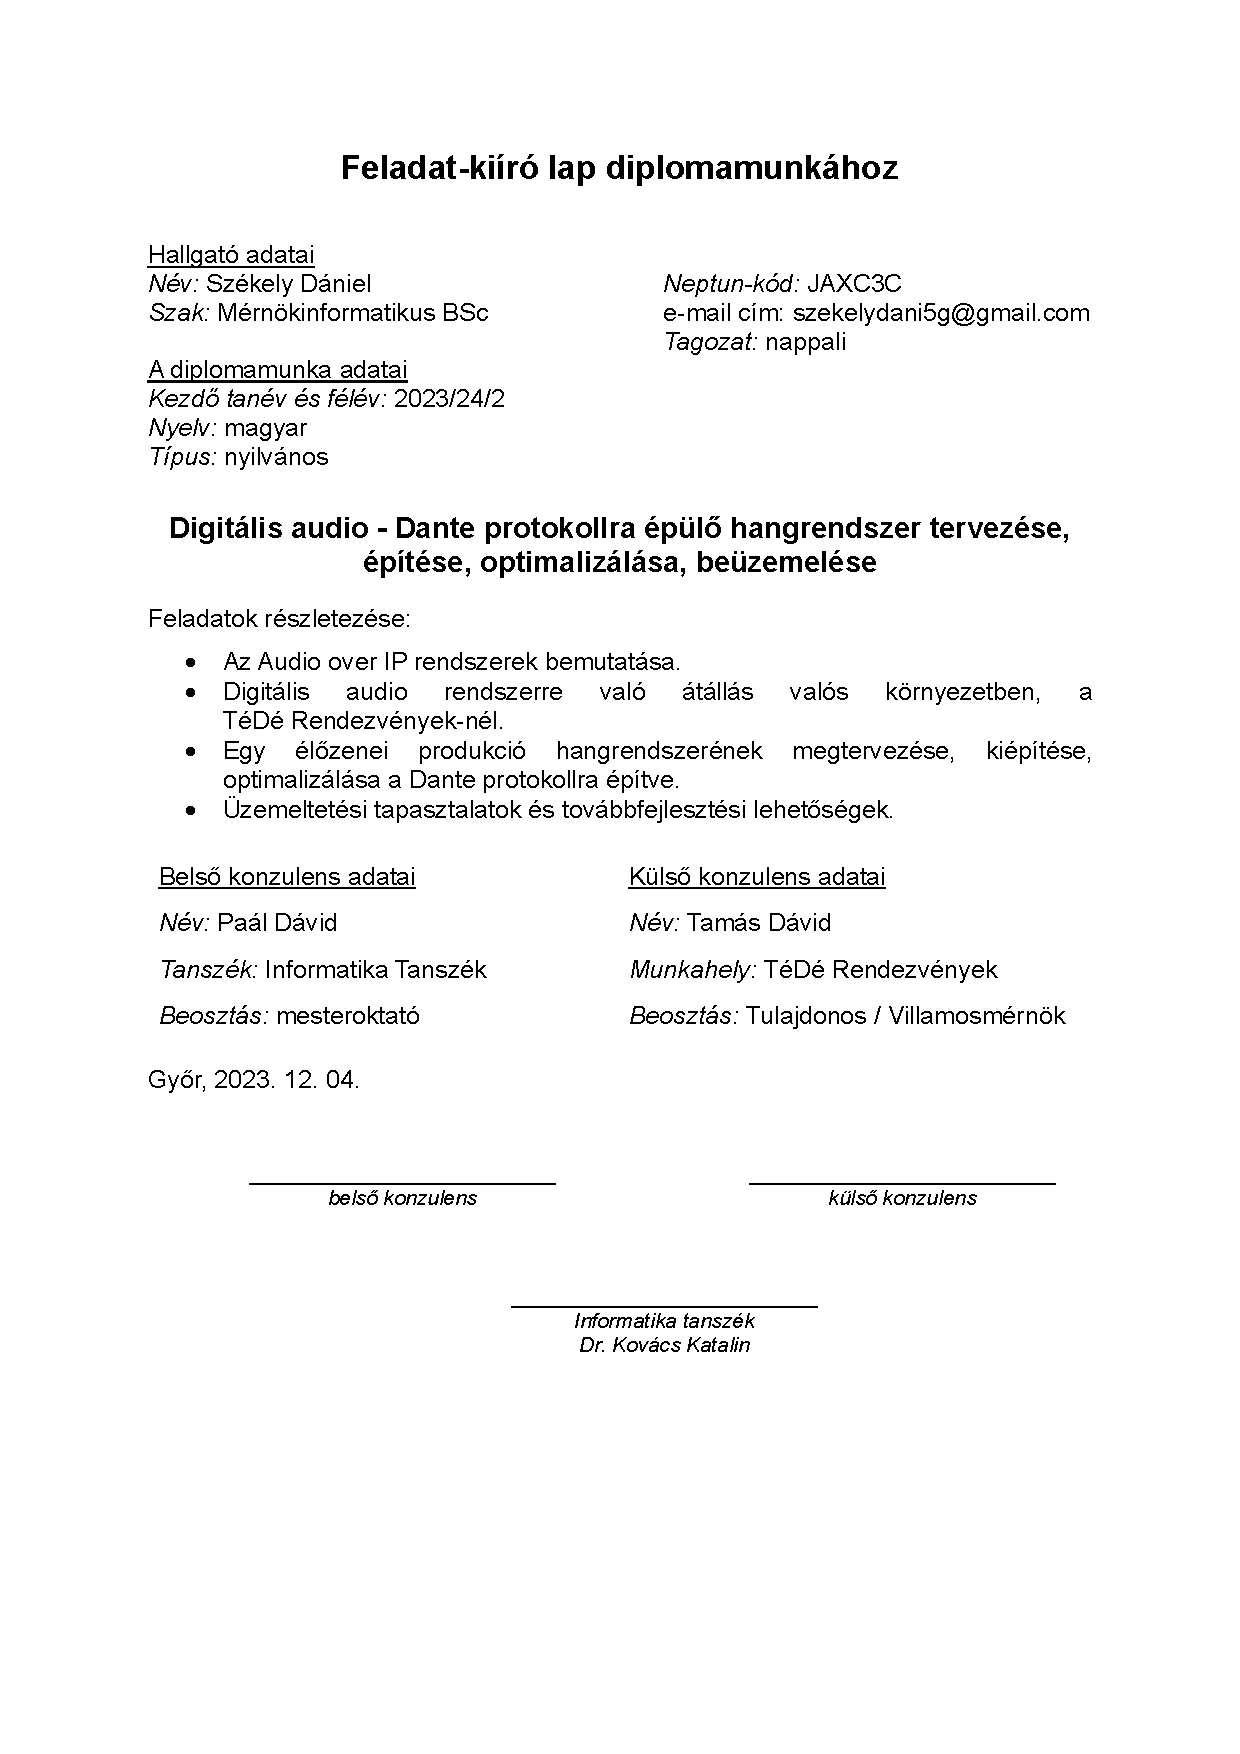
\includepdf{figures/start.pdf}

% Képfájlokhoz
\includegraphics*[width=\linewidth]{figures/start.png}


% Nyilatkozat és Kivonat
%~~~~~~~~~~~~~~~~~~~~~~~~~~~~~~~~~~~~~~~~~~~~~~~~~~~~~~~~~~~~~~~~~~~~~~~~~~~~~~~~~~~~~~
\selectlanguage{magyar}
\enfalse
\hutrue
\pagenumbering{gobble}
%--------------------------------------------------------------------------------------
% Nyilatkozat
%--------------------------------------------------------------------------------------
\chapter*{Nyilatkozat}

\noindent
Alulírott, \textbf{\szerzoVezeteknev{} \szerzoKeresztnev{} (\szerzoNeptun)}, \szak{} szakos hallgató kijelentem, hogy a \textit{\cim} című \MakeLowercase{\doktipus{}} feladat kidolgozása a saját munkám, abban csak a megjelölt forrásokat, és a megjelölt mértékben használtam fel, az idézés szabályainak megfelelően, a hivatkozások pontos megjelölésével.

\setlength\parskip{\baselineskip}

\noindent
Eredményeim saját munkán, számításokon, kutatáson, valós méréseken alapulnak, és a legjobb tudásom szerint hitelesek.

\vspace*{24pt}
\begin{multicols}{2}
	\noindent
	Győr, \emitdate{b}{\today}

	\columnbreak
	\noindent
	\makebox[7cm][c]{\rule{6cm}{.4pt}}\\
	\makebox[7cm][c]{\emph{\szerzoVezeteknev{} \szerzoKeresztnev}}\\
	\makebox[7cm]{hallgató}
\end{multicols}

\thispagestyle{empty}

\vfill
\clearpage
\thispagestyle{empty} % an empty page

\selectthesislanguage
 % ez legenerálódik magától a fentebb megadott adatok alapján
\pagenumbering{roman}
\setcounter{page}{1}

\selecthungarian

%----------------------------------------------------------------------------
% Kivonat Magyarul 
%----------------------------------------------------------------------------
\chapter*{Kivonat}
% TODO: Távolítsd el a megjegyzést, ha mégis szeretnéd, hogy bekerüljön a tartalomjegyzékbe
%\addcontentsline{toc}{chapter}{Kivonat}

Szakdolgozatom célja egy élőzenei produkció hangrendszerének megtervezése, 
kiépítése, optimalizálása és beüzemelése, mely a Dante protokollra 
építkezik. Az Audio over IP rendszerek, különösen a Dante hálózatok, 
lehetőséget nyújtanak a hagyományos analóg hangrendszerekhez 
képest gyorsabb, megbízhatóbb és skálázhatóbb megoldások alkalmazására. 

Az 1. fejezet bevezeti a szakdolgozat témáját és eredetét,
miért is ezt a témát választottam.

A 2. fejezet az alapvető hangtechnikai fogalmakat és rendszereket 
mutatja be, beleértve az analóg és digitális hangrendszerek 
közötti eltéréseket. 

A 3. fejezet célja, hogy alaposan bemutassa a digitális audió 
rendszerek alapjait és a Dante protokoll technikai részleteit. 
Ebben a részben többek között bemutatásra kerülnek az IP-címek kiosztásának módszerei, 
a hálózati topológiák kialakítása, 
valamint a különböző hálózati eszközök, mint például a switchek szerepei.

A 4. fejezet a tervezési és telepítési folyamatot tárgyalja, 
különös figyelmet szentelve a felhasznált eszközöknek, 
mint például a hangprocesszorok, végerősítők és 
hangszórók. 
A telepítés során a Dante alapú hálózat  kiépítése mellett kiemelten
foglalkozom a hangminőség optimalizálásával. A valós környezetben 
végzett tesztelés során a rendszer megbízhatóságát és 
rugalmasságát is értékelem.

Az 5. fejezet a telepítés utáni üzemeltetési tapasztalatokkal 
foglalkozik. Részletesen bemutatom a rendszer integrálását a 
TéDé Rendezvények egy élőzenei produkcióján, ahol 
valós időben teszteltem a Dante hálózat teljesítményét. 
Itt tárgyalom a hangrendszer és a vezérlőrendszerek 
integrációjának fontosságát, valamint az előadás közben 
tapasztalt akusztikai és hálózati kihívások kezelését. 
Az eredmények alapján további fejlesztési lehetőségeket 
javaslok, melyek még tovább növelhetik a rendszer teljesítményét és rugalmasságát.

Az általam bemutatott rendszer lényeges előnyöket nyújt egy analóg 
hangrendszerrel szemben.
Az üzemeltetési tapasztalatok azt igazolják, hogy 
az Audio over IP technológiák, különösen a Dante, 
stabil, skálázható és megbízható megoldást 
kínál a modern élőzenei produkciók számára.


\vfill
\selectenglish


%----------------------------------------------------------------------------
% Abstract in English
%----------------------------------------------------------------------------
\chapter*{Abstract}
% TODO: Távolítsd el a megjegyzést, ha mégis szeretnéd, hogy bekerüljön a tartalomjegyzékbe
%\addcontentsline{toc}{chapter}{Abstract}

The goal of my thesis is to design, build, optimize, and commission a sound system for 
a live music production based on the Dante protocol. Audio over IP systems, particularly 
Dante networks, offer faster, more reliable, and scalable solutions compared to traditional analog sound systems.

Chapter 1 introduces the topic and origin of the thesis, explaining why I chose this subject.

Chapter 2 presents the fundamental concepts and systems of sound technology, including 
the differences between analog and digital sound systems.

The purpose of Chapter 3 is to provide an in-depth overview of the fundamentals of 
digital audio systems and the technical details of the Dante protocol. This chapter 
includes topics such as methods for assigning IP addresses, designing network 
topologies, and the roles of various network devices, such as switches.

Chapter 4 discusses the design and installation process, with special emphasis on 
the equipment used, such as sound processors, amplifiers, and speakers. 
In addition to building the Dante-based network, I focus on optimizing sound quality 
during installation. During real-world testing, I evaluate the reliability and flexibility of the system.

Chapter 5 covers the operational experiences after installation. It details the 
integration of the system into a live music production by TéDé Rendezvények, where 
I tested the performance of the Dante network in real-time. 
This section highlights the importance of integrating the sound system with 
control systems and addresses the acoustic and network challenges encountered 
during the performance. Based on the results, I propose further development 
opportunities to enhance the system's performance and flexibility.

The system I present offers significant advantages over analog sound systems. 
Operational experiences confirm that Audio over IP technologies, particularly 
Dante, provide a stable, scalable, and reliable solution for modern live music productions.

\vfill
\selectthesislanguage

\newcounter{romanPage}
\setcounter{romanPage}{\value{page}}
\stepcounter{romanPage} %TODO ezt át kell írnod

% Tartalomjegyzék
%~~~~~~~~~~~~~~~~~~~~~~~~~~~~~~~~~~~~~~~~~~~~~~~~~~~~~~~~~~~~~~~~~~~~~~~~~~~~~~~~~~~~~~
\tableofcontents\vfill

% A dolgozat lényegi része
%~~~~~~~~~~~~~~~~~~~~~~~~~~~~~~~~~~~~~~~~~~~~~~~~~~~~~~~~~~~~~~~~~~~~~~~~~~~~~~~~~~~~~~
\pagenumbering{arabic}

% Saját munka
%----------------------------------------------------------------------------
\chapter{\bevezetes}
%----------------------------------------------------------------------------

%----------------------------------------------------------------------------
\section{A kezdetek}
%----------------------------------------------------------------------------

Kisgyermek koromtól kezdve érdekelnek a hangtechnikához fűződő eszközök és azok elméleti-gyakorlati működése. Első élményeim egyike közé tartozik az, amikor
szüleim egy új fajta rádiólejátszót vásároltak otthonra, amelyen már nem csak a rádióadásokat lehetett hallgatni, hanem lejátszhatóak voltak kazetták is.
A készüléket akkoriban jobban tudtam kezelni gyermekként, mint a szüleim, egyértelmű volt már akkoriban is, a technika és a zene iránti érdeklődésem.
Ezek után általános iskolában a fizika tanárommal együtt kezdük el a sulirádió működtetését, amelynek a telepítési részében is részt vettem, mivel azelőtt
csak egyszerű csengők voltak felszerelve az épületben. Szükség volt hangsugárzókra, erősítőkre, mikrofonokra, és egyéb kiegészítőkre. A rádió működtetése
is az én feladatom lett két másik barátommal együtt, az iskolával kapcsolatos híreket és információkat mondtuk be rövid szünetekben, a hosszabb szünetekben pedig zenéket játszottunk.
Mindeközben zeneiskolába is beiratkoztam, ahol ütőhangszeresként tanultam egészen egyetemi tanulmányaim kezdetéig. A több mint tíz év alatt, sok új ismeretet és tapasztalatot szereztem,
amit a későbbiekben mint zenész, mint hangosító tudtam hasznosítani. Megismerkedtem a különböző zenei stílusok egyedi hangzásvilágával, ami a későbbiekben a hangosításban is nagy segítségemre volt.
Középiskolai tanulmányaim alatt kezdtem el komolyabban foglalkozni a hangtechinka világával komolyabb szinten. 
A fizika tanárommal ugyanis korábban nem csak a sulirádiót működtettük, hanem az összes sulibulit és rendezvényt a faluban mi szolgáltuk ki technikailag.
Ezért mivel már középiskolába jártam, a későbbiekben egy feltörekvő fiatalos és modern gondolkodású magánvállalkozáshoz ajánlott be engem, mivel a fiatal és motivált munkaerőt kerestek. (TéDé Rendezvények)
Már az első munkalehetőségnél éreztem, hogy ez egy nagyon jó lehetőség számomra, mindenképpen szeretnék ebben a szakmában dolgozni.
A cég fő profilja a hangrendszerek kiépítése és üzemeltetése volt, de későbbiekben már a fénytechnikával és színpadtechnikával is el kezdtünk foglalkozni. 
Ettől kezdve kezdtem el aktívan dolgozni a rendezvényiparban a hangrendszerek világában. Az évek során egyre több tapasztalatot
szereztem. Évente több mint száz rendezvényen tudtam folyamatosan fejlődni, rutint és ismerettséget szerezni a szakmában.

\subsection{Téma választás}

A hangrendszerek világa az elmúlt években nagy változáson ment keresztül. A digitális technika térhódítása a hangtechnikában is megjelent, és egyre több fajta megoldás jelent meg a piacon.
A digitális fejlesztésekből mi sem szerettünk volna kimaradni, hogy hangtechnikai apparátusunk korszerű és versenyképes maradjon.
Ekkor jött a fejlesztési ötlet, egy olyan rendszert tervezni, amely teljes mértékben digitális alapokra helyezi a jelenlegi hibrid megoldásunkat. A cégvezetőtől azt a feladatot kaptam,
hogy tervezzek egy olyan rendszert, amely megoldja a jelenlegi hibrid rendszerünk teljes digitális megoldásra való cseréjét. 
Az alapvető szempontok közé tartozott, hogy a rendszer legyen könnyen skálázható, és bővíthető, valamint a jelenlegi rendszert minden tekintetben felülmúlja.
Első lépésben a különböző Audio over IP protokollok közül kellett választanom,
amely a leginkább megfelel a rendszerünk igényeinek. Ehhez a piacon lévő protokollokat kellett megvizsgálnom, és a legjobb megoldást választani. 
Szakdolgozatomban sok idegen nyelvű szóra nincsen megfelelő és pontos fordítás ami teljes mértékben tükrözné az adott kifejezés jelentését.
A továbbiakban ebből kifolyólag feltételezve azt, hogy az olvasó tisztában van a szakmai terminológiával angolul fogom említeni a szakmai kifejezéseket.
Ezek a kifejezések megjelenhetnek írt szövegként és ábrás illusztrációkban is.

%----------------------------------------------------------------------------
\chapter{\AudioBasics}
%----------------------------------------------------------------------------

\begin{comment} 
Annak érdekében, hogy a későbbi fejezetekben a hangtechnikai rendszerek működését és tervezését megérthessük,
először szükséges a hangtechnikai alapok ismerete. Ez a fejezet a későbbi fejezetekben használt alapfogalmakat definiálja röviden és tömören.

%----------------------------------------------------------------------------
\section{Mikrofon típusok}
%----------------------------------------------------------------------------

A mikrofon egy eszköz, amely az akusztikus energia hangterét elektromos energiává alakítja át.
Az eszköz érzékelheti a hangnyomást vagy a hangnyomás gradienst, amely arányos a hangsebességgel (mindkettő kombinációja a hangintenzitásnak).
Négy különböző átalakítótípus létezik, amelyeket reciprok transzducerekként használhatunk mikrofonokhoz:

% ----------------------------------------------------------------------------
\begin{itemize}
    \item Kapacitív transzducer
    \item Piezoelektromos transzducer
    \item Dinamikus transzducer
    \item Mágneses transzducer
\end{itemize}
% ----------------------------------------------------------------------------

Az említett összes transzducer lehetővé teszi a mechanikai rezgések elektromos rezgésekké történő átalakítását,
miközben különböző elveket követnek. Az első kettő esetében az elektromos mező változása
van használatban, míg az utolsó kettő esetében egy vezetőben keletkező áram indukciója a mágneses térben történő vezetékmozgás révén,
vagy a mágneses fluxus változása egy tekercsen. 
Elsősorban a négy említett transzducer közül kettőt a kapacitív és a dinamikus transzducert
használjuk gyakorlati jelentőséggel a rendezvénytechnikában.

% ----------------------------------------------------------------------------
\subsection{Dinamikus mikrofon}
% ----------------------------------------------------------------------------

A dinamikus mikrofonok a legelterjedtebb mikrofonok a hangtechnikában.
A hangnyomás mechanikai rezgéseit alakítják elektromos jelekké, elve, hogy egy membrán mely egy tekercsre van rögzítve, és ez mágneses mezőben mozog.
A membrán rezgése a tekercsben elektromos feszültséget indukál, amely a hangjelet reprezentálja.
Nagyon strapabíróak és megbízhatóak, széles körben használják őket élő hangosításban és stúdiótechnikában.
Hátránya a kisebb frekvenciaátvitel és a nagyobb torzítás.
Az egyik legismertebb dinamikus mikrofon a Shure SM57, amely egy nagyon népszerű mikrofon a hangtechnikában, és sokféle alkalmazásban használják.

% ----------------------------------------------------------------------------
\begin{figure}[H]
    \centering
    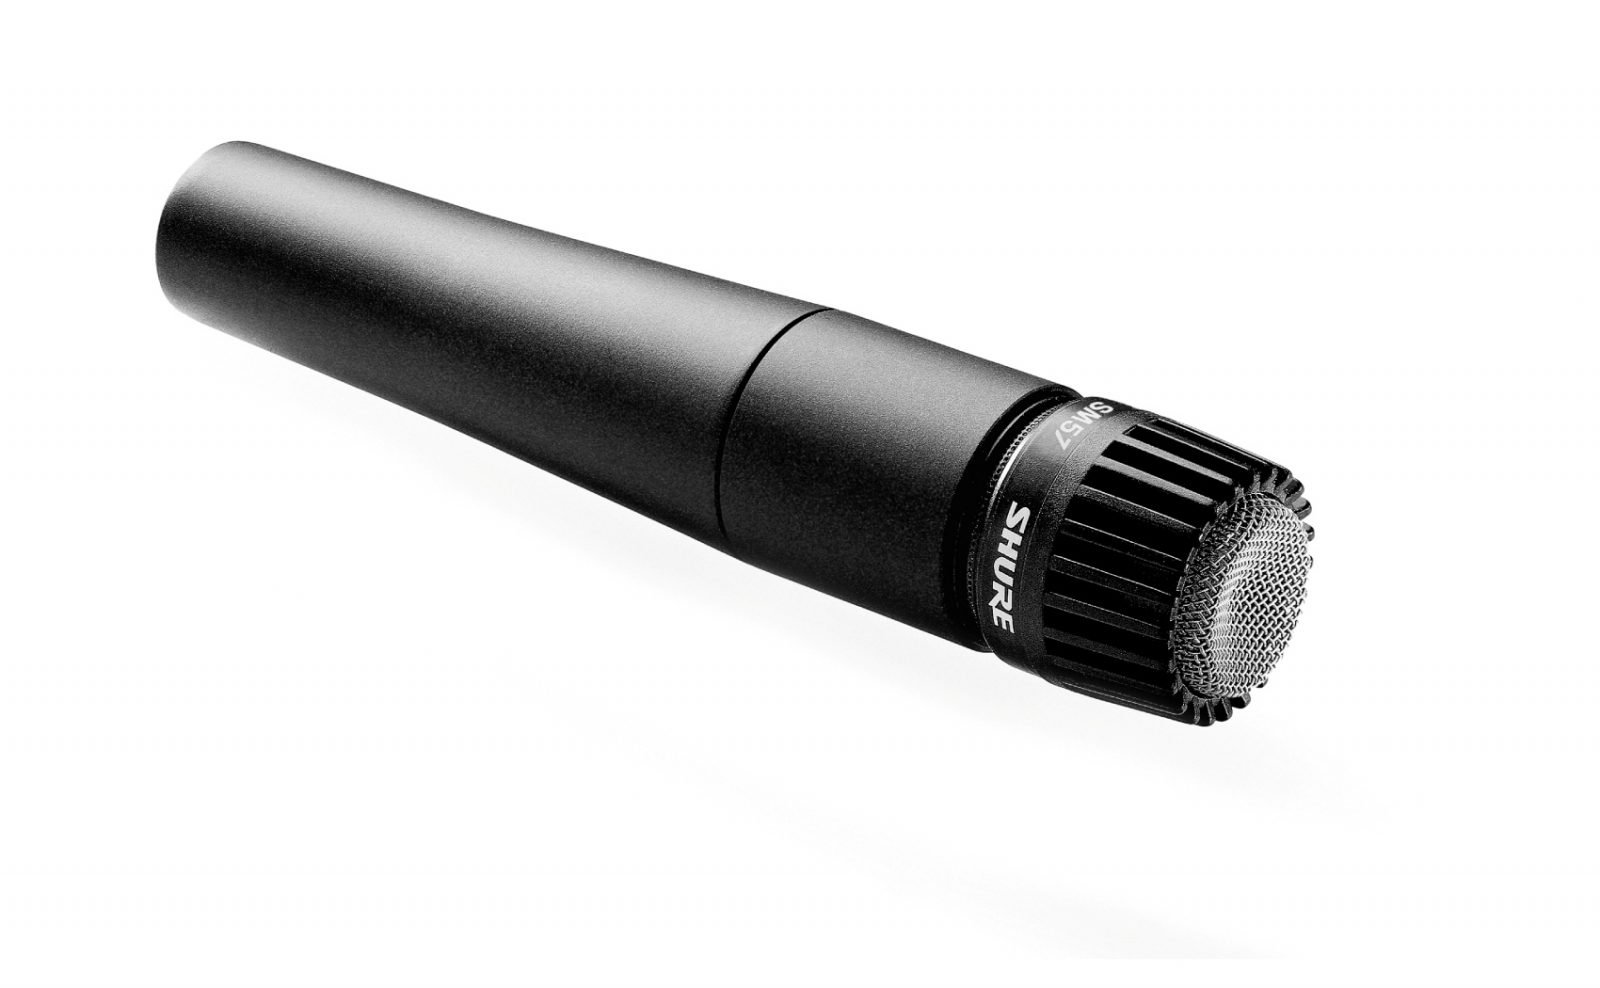
\includegraphics[width=0.3\textwidth]{figures/shure-sm57.jpg}
    \caption{Shure SM57 dinamikus mikrofon}
    \label{fig:shure_sm57}
\end{figure}
% ----------------------------------------------------------------------------

 
% ----------------------------------------------------------------------------
\subsection{Kondenzátor mikrofon}
% ----------------------------------------------------------------------------

A kondenzátor mikrofonok a nagyobb frekvenciaátvitellel rendelkező mikrofonok, és a nagyobb dinamikatartományt is képesek lefedni.
A hangnyomás a membrán rezgéseit egy kondenzátorban változó kapacitásként alakítja át, amelynek egyik eleme a membrán, a másik pedig egy fix elektromosan töltött lemez.
A membrán rezgései a kapacitás változását okozzák, amely a hangjelet reprezentálja.
A kondenzátor mikrofonok nagyon érzékenyek, és nagyon jó hangminőséget biztosítanak.
Azonban a kondenzátor mikrofonoknak van néhány hátránya is, például az áramellátás szükségessége, a magasabb ár és a nagyobb méretek.
Egy példa a kondenzátor mikrofonra a Shure SM137 kondenzátor mikrofon, amely egy elterjed mikrofon a hangtechnikában.

% ----------------------------------------------------------------------------
\begin{figure}[H]
    \centering
    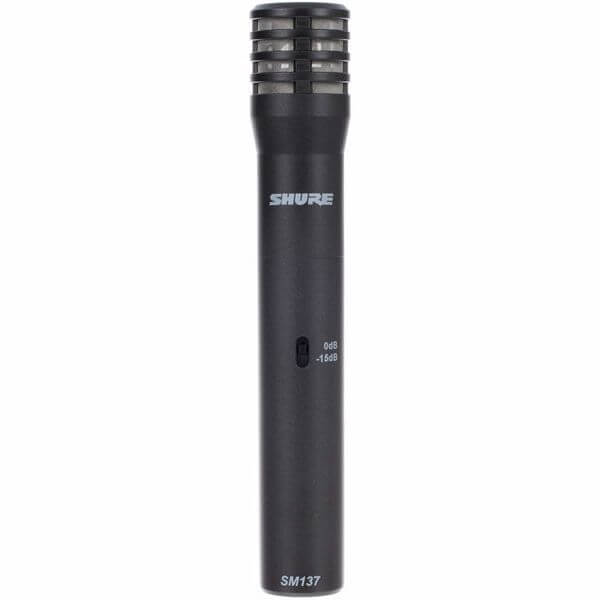
\includegraphics[width=0.3\textwidth]{figures/shure-sm137.jpg}
    \caption{Shure SM137 kondenzátor mikrofon}
    \label{fig:shure_sm137}
\end{figure}
% ----------------------------------------------------------------------------
\end{comment}

% ⛔📝 TODO: Merge text formatting and content integration check

%----------------------------------------------------------------------------
\section{Az analóg kezdetek} % Kezdeti analóg rendszerek, skálázhatósági hátrányok, analog rendszerek korlátai, működési alapelvek, technológiai háttér  
%----------------------------------------------------------------------------
Az analóg hangrendszerek története az audio technológia hajnalára nyúlik vissza. 
Az ilyen rendszerek alapját az elektromos analóg jelek képezik, amelyek az akusztikus hangot elektromos árammá alakítják,
a hangjelet közvetlenül, torzítás nélkül próbálják átadni az erősítőnek majd ezáltal hangszóróknak.
Az analóg rendszerek egyik legfontosabb alapelve az elektromos jelek folyamatos feldolgozása. 
A hangot analóg módon rögzítik, és az áramkörök szigorú tervezése biztosítja, hogy az eredeti akusztikus jel minél pontosabban tükröződjön az outputban.
A legnagyobb hátrány az analóg rendszerek skálázhatóságában rejlik. 
Ahogy a rendszer bonyolultsága nőtt, úgy a karbantartás és az állandó finomhangolás is egyre több problémát okozott. 
Az analóg technológiáknál a jel erősítése és kezelése gyakran jelentős torzulásokat és zajokat okozott, amelyeket nehéz volt kezelni.
A kábelezést tekintve sem volt egy leányálom az analóg rendszerek használata, mivel a nagyobb távolságokon a jel torzulása és a zajok könnyen bekerülhettek a rendszerbe.
Egy sokcsatornás produkciónál szép spagettiláncokat is eredményezett, még a legtapasztaltabb hangmérnökök számára is kihívást jelentett. 
Továbbá, a rendszer hibái nem mindig voltak könnyen diagnosztizálhatók, ami a szervizelési időket jelentősen megnövelte.
A hangrendszerek technológiai hátterét tekintve, az analóg rendszerekben a transzformátorok, kondenzátorok és ellenállások kulcsszerepet játszottak. 
Ezek az alkatrészek feleltek a jel szűréséért, erősítéséért és átalakításáért. 
Azonban ezek az elemek gyakran voltak érzékenyek a környezeti hatásokra, mint például a hőmérséklet-ingadozások és a páratartalom, 
amelyek további kihívások elé állították a hangmérnököket.
%----------------------------------------------------------------------------
\section{Digitális térhódítás} % Miért digitális irányba fejlesztünk és halad az ipar? Miért jobb mint az analog? 
%----------------------------------------------------------------------------
A digitális technológia térhódítása a professzionális audio rendszerekben jelentős paradigmaváltást hozott az audioiparban. 
Az utóbbi évtizedekben a digitális rendszerek folyamatosan felváltották az analóg megoldásokat, számos előnnyel rendelkezve, 
amelyek hozzájárultak a hangtechnikai rendszerek fejlődéséhez. 
Az egyik legfontosabb tényező, amely a digitális technológia előnyére szolgál, a jelminőség és a stabilitás drasztikus javulása. 
A digitális rendszerekben a hangjelek bitstream formájában kerülnek feldolgozásra, amely lehetővé teszi a zajok és torzítások minimalizálását,
a jelfeldolgozás során. 

A digitális rendszerek jelentős előnye, hogy magasabb jel-zaj viszonyt biztosítanak, amely fokozza a jel tisztaságát és mérsékli a zavaró hatásokat. 
Ezáltal a hangminőség jelentős javuláson megy keresztül, mivel a digitális feldolgozás során a hasznos jel és a 
háttérzaj közötti különbség egyértelműbbé válik.
Szélesebb dinamikatartományt nyújt, amely lehetővé teszi a nagyobb hangerő eltérések hatékony kezelését. 
A digitális rendszerek egyik további előnye, hogy a digitális adatok másolása során nem történik minőségromlás. 
A másolatok pontosan ugyanolyan minőséget képviselnek, mint az eredeti felvétel, így garantált a tökéletes reprodukálás.
Stabil működést biztosítanak változó hőmérsékleti és tápfeszültség-ingadozások mellett. 
Az analóg rendszerek által okozott torzulások elkerülhetőek, így nincs jelen jeltorzulás a digitális rendszerekben.
Képesek kezelni az együttfutás és hangmagasság-ingadozás problémáit, amelyeket az analóg rendszerek nehezebben tudnak kezelni.
A digitális rendszerek emellett képesek visszaállítani az egyenfeszültségű jelkomponenseket, és biztosítják 
a lineáris frekvenciamenetet, amely pontos hangátvitelt eredményez. 
%----------------------------------------------------------------------------
\subsection{PCM - Pulse Code Modulation}
%----------------------------------------------------------------------------
A hangfrekvenciás jelek digitális feldolgozása a PCM (Pulse Code Modulation, impulzuskód-moduláció) elvén alapul. 
Ennek során az analóg jelet diszkrét impulzusok sorozatára bontják, ahol az impulzusok 
amplitúdóértékei bináris kódokkal kifejezett információt hordoznak.

A PCM jel előállítása az A/D (analóg-digitális) átalakításon keresztül történik. 
Az analóg jelek időbeli és értékbeli folytonossága diszkrét minták sorozatává alakul, 
miközben az információtartalom megőrzi az eredeti jelhez hasonló értékét. 
Ezt a mintavételi tételt (C. E. Shannon) bizonyította, amely alapján az eredeti jel 
visszaállítható információveszteség nélkül, ha a mintavételi frekvencia legalább 
kétszerese az analóg jel legmagasabb frekvenciájának.

Az analóg jelben előforduló maximális frekvenciát Nyquist frekvenciának nevezik. 
Ennek megfelelően a mintavételi frekvencia határozza meg a digitális hangfeldolgozó rendszer sávszélességét. 
Figyelembe véve, hogy a hangfrekvenciás jel felső határa 20 kHz, a hifi hangminőség eléréséhez a 
mintavételi frekvencia minimálisan 40 kHz-nél nagyobb kell hogy legyen. A digitális hangfeldolgozás során jellemző mintavételi frekvenciák az alábbiak:
%----------------------------------------------------------------------------
\begin{itemize}
    \item CD minőség: 44.1 kHz
    \item DVD minőség: 48 kHz
    \item Studio minőség: 96 kHz
    \item Ultra minőség: 192 kHz
\end{itemize}
%----------------------------------------------------------------------------
A digitális hangfelvételek bitmélysége az analóg jelből származó egyes minták tárolásához 
felhasznált számjegyek számát jelöli. A CD hangformátum esetében a szabványos bitmélység 16 bit, 
míg a mintavételi frekvencia 44,1 kHz. Ez azt jelenti, hogy másodpercenként 44 100 hangmintát rögzítenek, 
és minden egyes minta 16 bitnyi információt tartalmaz. 
Bár a nagyobb bitmélység általában jobb hangminőséget biztosít, ez egyúttal nagyobb fájlmérettel is jár.
A digitális hangfeldolgozás során jellemző bitmélységek az alábbiak:
%----------------------------------------------------------------------------
\begin{itemize}
    \item CD minőség: 16 bit
    \item Studio/live minőség: 24 bit
    \item Ultra minőség: 32 bit
\end{itemize}
%----------------------------------------------------------------------------
\begin{figure}[H]
	\centering
	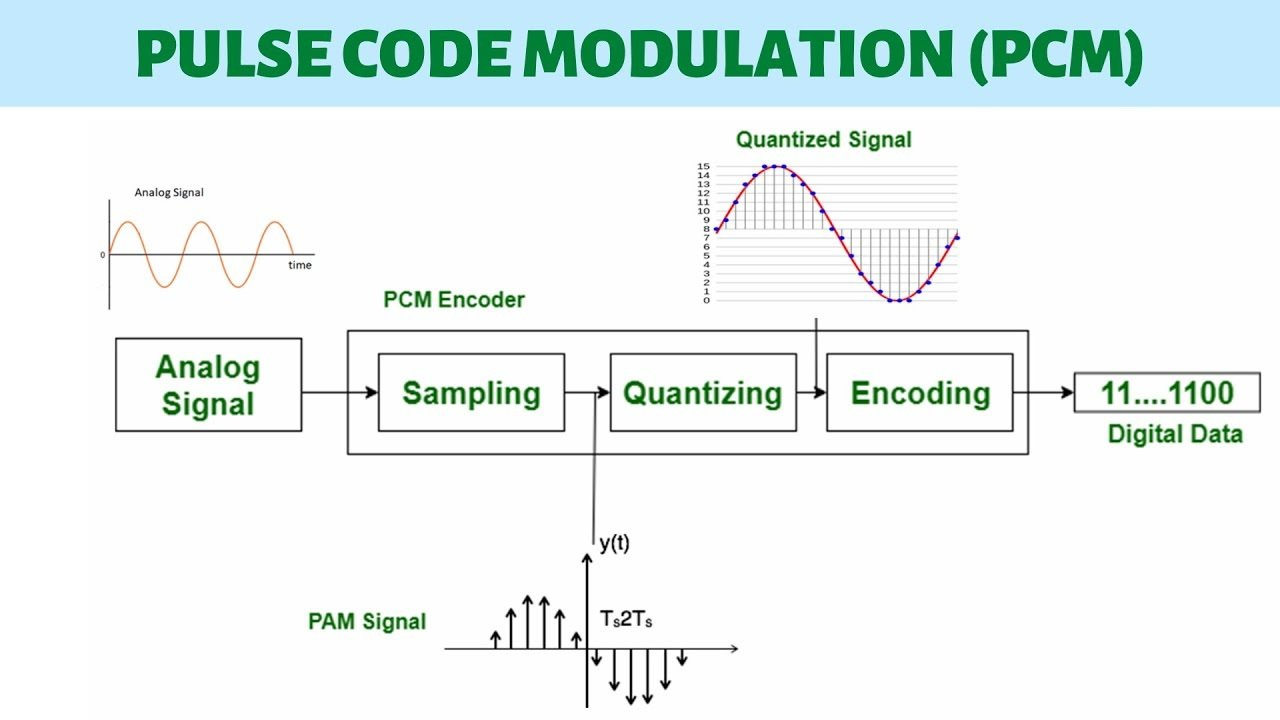
\includegraphics[width=\linewidth, keepaspectratio]{figures/pulse _code_modulation.jpg}
	\caption{Pulse Code Modulation (PCM) folyamat~\cite{PULSECODEMODULATION}}\label{fig:pcm}
\end{figure}
%----------------------------------------------------------------------------
A digitális hangfeldolgozás területén fontos szerepet játszik az A/D átalakítók kialakítása, 
a kódolás folyamata, a D/A (digitális-analóg) átalakítás, valamint a hibafelismerés és hibajavítás.
%----------------------------------------------------------------------------
\subsection{ADC és DAC konverterek - mintavételezés}
%----------------------------------------------------------------------------
A mintavételezés olyan folyamat, amely során egy analóg hangjeleket digitális formába alakítanak át, azaz mintákat vesznek az időben folytonos hanghullámokból. 
Ez az alapja annak, hogy a hangot számítógépes rendszerekben kezelni lehessen. A hangminták gyakorisága meghatározza a mintavételi frekvenciát, 
ami meghatározza a digitális hangminőséget és a frekvencia tartományt. Általában minél magasabb a mintavételi frekvencia, annál jobb a hangminőség, 
de nagyobb sávszélességet is eredményez.

A digitalizálási folyamat során időbeli mintavételezés történik. 
Folyamatos mintavételezéskor a hang intenzitásával arányos diszkrét értékek, azaz feszültségimpulzusok jönnek létre. 
A mintavétel során az impulzusok a beérkező amplitúdó értékek alapján végtelen számú értéket vehetnek fel, 
ám a rendelkezésre álló bináris adatszók száma véges. Ezt a jelenséget kvantálásnak vagy tartományokba 
való felosztásnak nevezzük.

A kvantálás során a hangtartomány véges számú lépcsőre oszlik. 
A kvantálás finomsága, amely a mintavételi frekvenciával együtt a digitális jelfeldolgozás 
egyik legfontosabb paramétere, meghatározza a hang digitalizálásának részletességét. 
A kvantálásnál figyelembe kell venni a kvantálási zajt is, amely a tartományok növelésével csökkenthető.
A kvantálási zaj olyan zavaró tényező, amely a digitális hangrögzítés vagy lejátszás során jelentkezik, 
és a kerekítési hibák következményeként alakul ki. Ez a zaj a különbség az eredeti analóg jel és a 
digitális formában ábrázolt jel értékei között, amit a digitális eszközök kvantálási folyamatában jelentkező pontatlanságok okoznak.
A kvantálási zaj keletkezése a digitális jel analóg formából történő diszkrét értékekre (kvantumokra) 
történő átalakítása során jelentkező kerekítési hibákra vezethető vissza. 
E hibák következtében a kvantálási zaj nemlineáris harmonikus torzítás formájában jelenik meg, ez a hangminőség romlásához vezető zavaró tényező.

A kvantálási zaj csökkentésére több módszer létezik. Az egyik lehetséges megoldás a 
digitális jel dinamikatartományának növelése. Amennyiben a kvantálási pontosságot 
egy bittel növeljük, a jel-zaj viszony javulhat, és ezzel együtt a dinamika is +6 dB-el növekedhet. 
Továbbá, a zajcsökkentő algoritmusok alkalmazása és a magas felbontású digitális konverterek használata szintén hozzájárulhat a kvantálási zaj mérsékléséhez.
A kódolás során a hangszintek szerint kvantált pontok kódkombinációk sorozataként, digitális jelekként jelennek meg.

Az ADC (Analog-to-Digital Converter) konverter az analóg hangjeleket digitális jelekké alakítja át, míg a DAC (Digital-to-Analog Converter) 
konverter a digitális jeleket visszaalakítja analóg hangjelekké. 
A professzionális ADC és DAC konverterek nagymértékben befolyásolják a hangminőséget.
%----------------------------------------------------------------------------
\section{Hangerősség és hangnyomásszint} % Mi a hangerősség és a hangnyomásszint? Hogyan mérjük őket? Mi a különbség közöttük?
%----------------------------------------------------------------------------
Hangerőség (Intenzitás):
A hangerősség az a szubjektív hangosságérzet, amely a fizikai hangnyomás szintjétől függ. 
Ennek mértéke phonban van kifejezve, ahol a hangerőség értéke annyi phon, ahány dB-t mérünk 
egy 1 kHz-es szinuszhang hangnyomásszintjén, amely azonos hangosságérzetet kelt.

Hangosság (Hangnyomásszint):
A hangosság az egyidejűleg megszólaló hangok összefoglaló mértékét jelöli, amelyet a sone egységében mérünk. 
A kiszámítása során, ha a hangerősség meghaladja a 40 phon értéket, a hangosságot sone-ban adják meg.

A dB-skála a hangnyomásszint logaritmikus kifejezésére szolgál. Az emberi hallás érzékenysége különböző 
frekvenciákon eltérő, és a decibelskála lehetővé teszi, hogy az emberi hallás által 
érzékelhető hangnyomás tartományát pontosan ábrázoljuk.
A hangosság és a hangerőség közötti eltérés abban rejlik, hogy míg a hangosság az emberi érzékelésre, 
vagyis az érzékelhető hangnyomásra vonatkozik, addig a hangerőség a hanghullámok 
fizikai tulajdonságait, vagyis a hullámokban terjedő energiát méri.
\begin{comment}
%----------------------------------------------------------------------------
\begin{figure}[H]
	\centering
	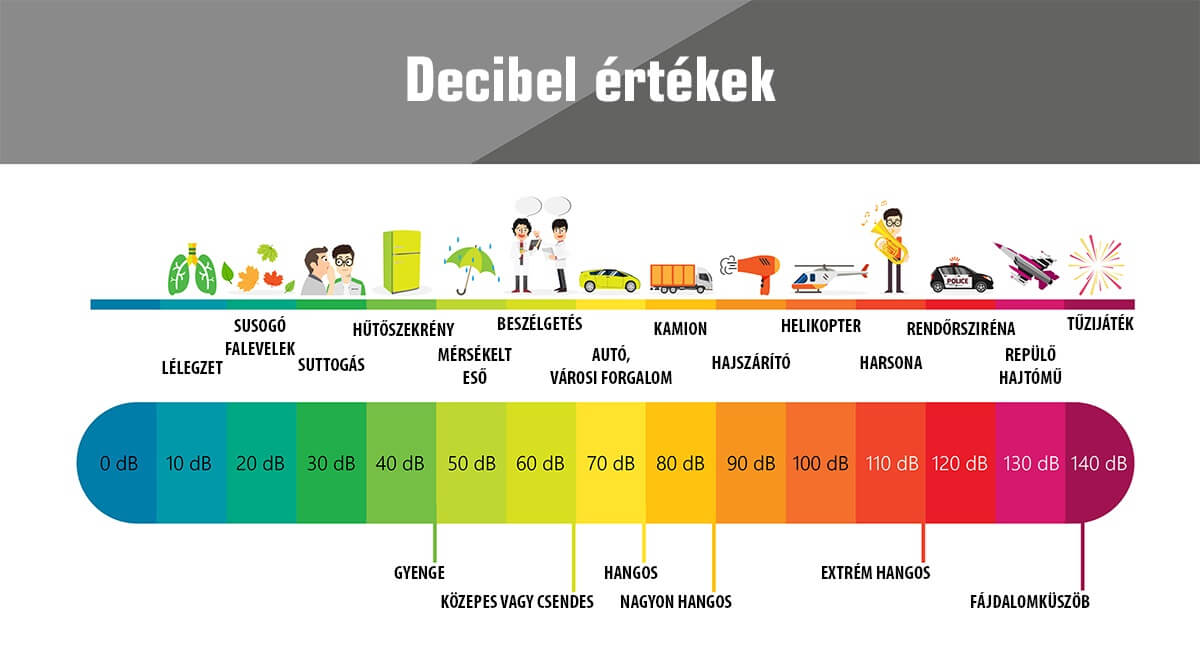
\includegraphics[width=\linewidth, keepaspectratio]{figures/db_scale.jpg}
    \caption{Decibel skála~\cite{DECIBELSCALE}}\label{fig:db_scale}
\end{figure}
%----------------------------------------------------------------------------
\end{comment}
Az emberi fül által észlelt legkisebb hangerősség 0 dB, amely alig érzékelhető. 
A 50 dB körüli hangerőt kellemesnek találjuk, míg a 100 dB-es szint már kellemetlenséget 
okozhat. A fájdalomküszöb nagyjából 140 dB-nél helyezkedik el. Érdemes megjegyezni, hogy 
a 100 dB nem kétszerese az 50 dB-nek hangerősség szempontjából. A hangerő érzékelése 
szubjektív, és az egyéni hallási képességek határozzák meg. Általában egy 10 dB-es 
növekedést körülbelül kétszer olyan hangosnak érzékelünk, tehát egy 60 dB-es hangerőt 
körülbelül kétszer hangosabbnak érzünk, mint az 50 dB-eset. Mivel a decibelskála logaritmikus 
alapú, a dB-ben megadott értékek nem lineárisan arányosak. Például a 120 dB nem kétszerese 
a 60 dB-nek, hanem a hangnyomása hozzávetőlegesen ezerszer nagyobb. 
%----------------------------------------------------------------------------
\begin{figure}[H]
	\centering
	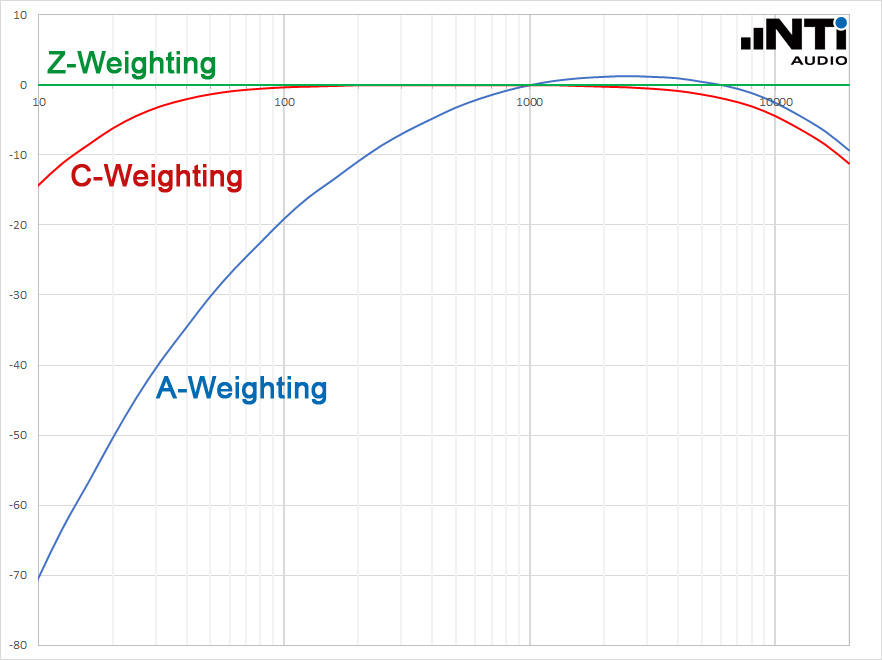
\includegraphics[width=350px, keepaspectratio]{figures/db_weights.jpg}
    \caption{A-, C- és Z-súlyozás~\cite{DBWEIGHTS}}\label{fig:db_weights}
\end{figure}
%----------------------------------------------------------------------------
A hangnyomás mérésére különböző súlyozási görbéket alkalmazhatunk, például A, C és Z súlyozást. Mit is jelentenek 
ezek? Ha egy hang az összes frekvenciatartományban egyenlő hangnyomással rendelkezik, azt a 
Z-súlyozási görbe segítségével ábrázolhatjuk. Az emberi fül által észlelt hangokat az 
A-súlyozási görbe írja le, amely pontosan tükrözi az emberi hallás frekvenciatartományát, mivel 
az emberi hallás nem érzékel minden frekvenciát egyformán. A C-súlyozás a hangélményt 
reprezentálja, amikor a hangerő növekedésével az alacsonyabb frekvenciák iránti érzékenység is 
fokozódik. Az A- és C-súlyozás tehát a leginkább megfelelő az emberi hallás valósághű 
frekvenciaválaszának modellezésére.

\newpage
\section{Pontsugárzó és LineArray hangforrások} % Mi a különbség a pontsugárzó és LineArray hangforrások között? Milyen alkalmazási területeken használjuk őket?
%----------------------------------------------------------------------------
Hangládák kiválasztásakor a legelterjedtebb formátumok a pontsugárzó és a Line Array rendszerek.
Ez a két típusú hangforrás eltérő működési elvekkel rendelkezik, 
amelyek befolyásolják megfelelő alkalmazási területeiket és a hangzás minőségét.
A pontsugárzó hangszórók, jellemzően kisebb eseményeken, 
otthoni környezetben és egyes konferenciákon találhatók meg. Ezek a hangszórók egyetlen 
dobozból állnak, amelyben minden szükséges komponens elhelyezésre került a hang előállításához. 
A pontsugárzók a hangot minden irányba terjesztik, olyan módon, mintha a hang egyetlen pontból áramlana ki. 
Könnyen telepíthetők és jól alkalmazhatók kisebb rendezvényekhez. Különböző méretűek 
lehetnek, a kis asztali hangszóróktól kezdve a nagyobb DJ-rendszerekig.
%----------------------------------------------------------------------------
\begin{figure}[H]
	\begin{minipage}{0.5\textwidth}
		\centering
		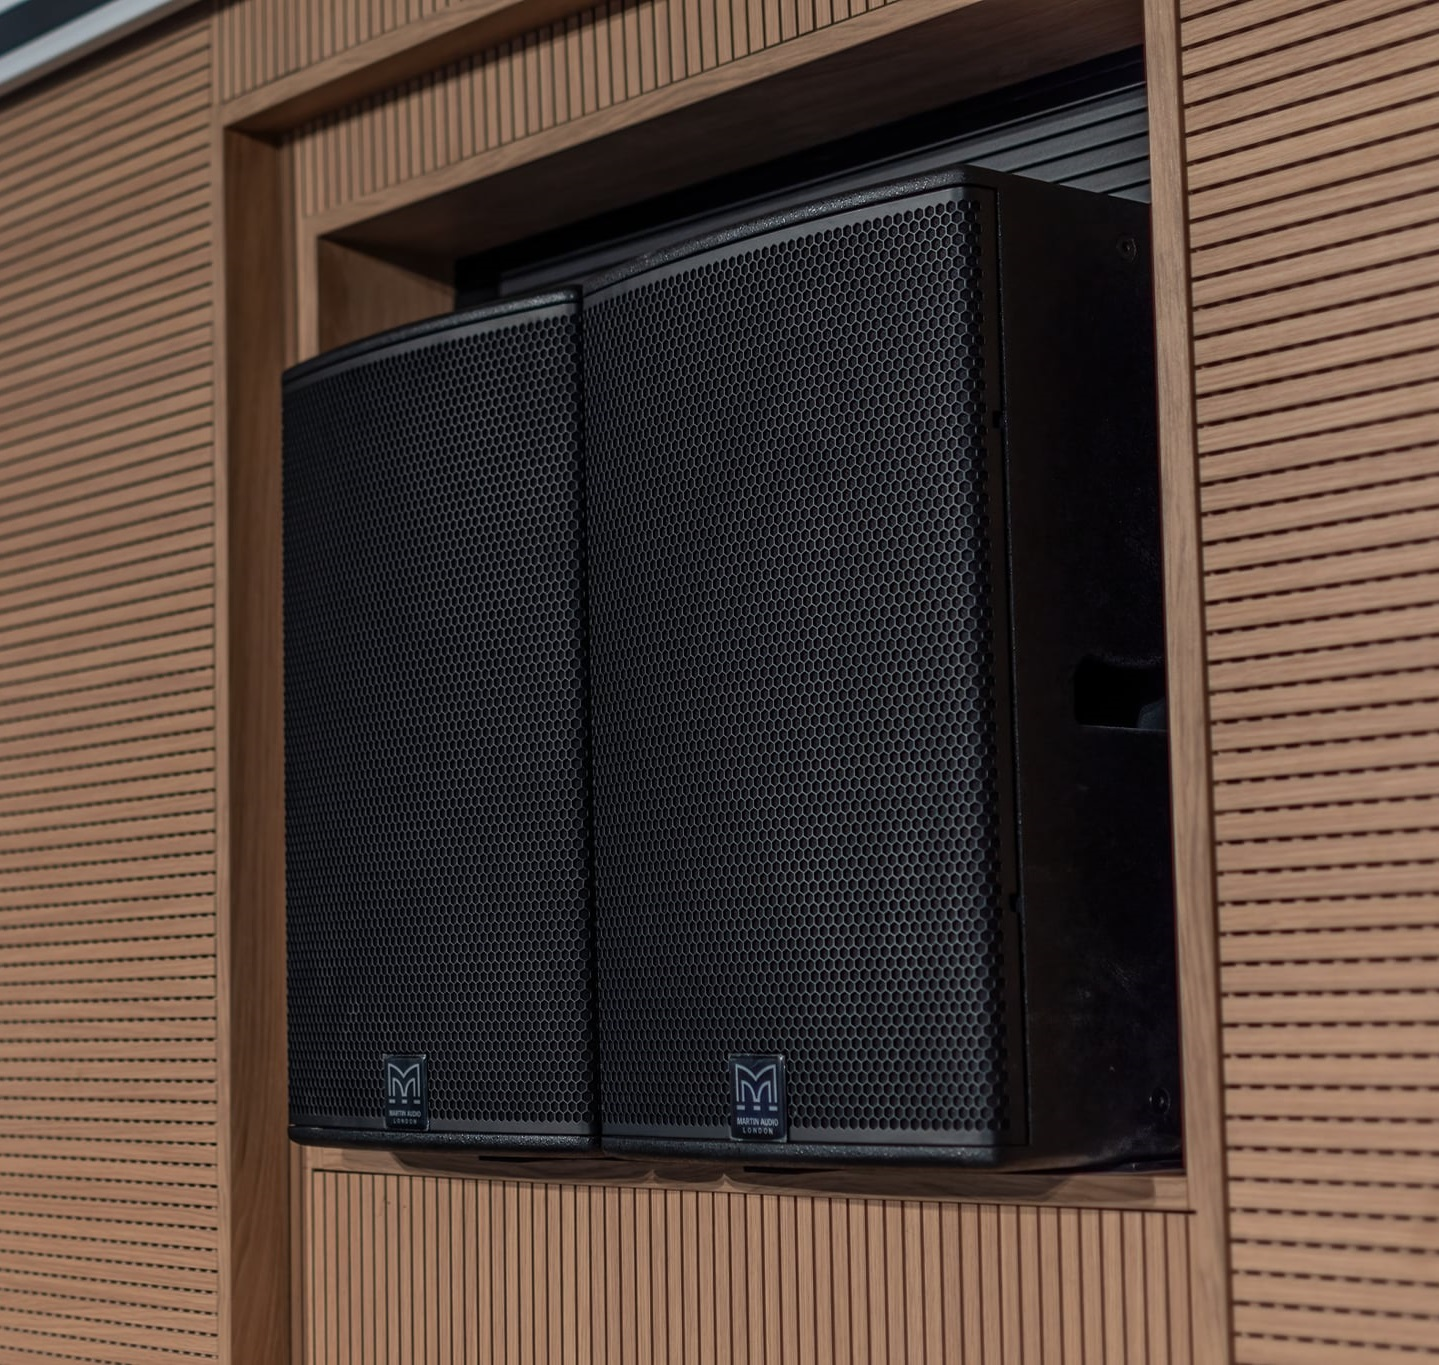
\includegraphics[width=150px, keepaspectratio]{figures/point_source.jpg}
        \caption{Pontsugárzó rendszer}
        \label{fig:point_source}
	\end{minipage}%
	\begin{minipage}{0.5\textwidth}
		\centering
		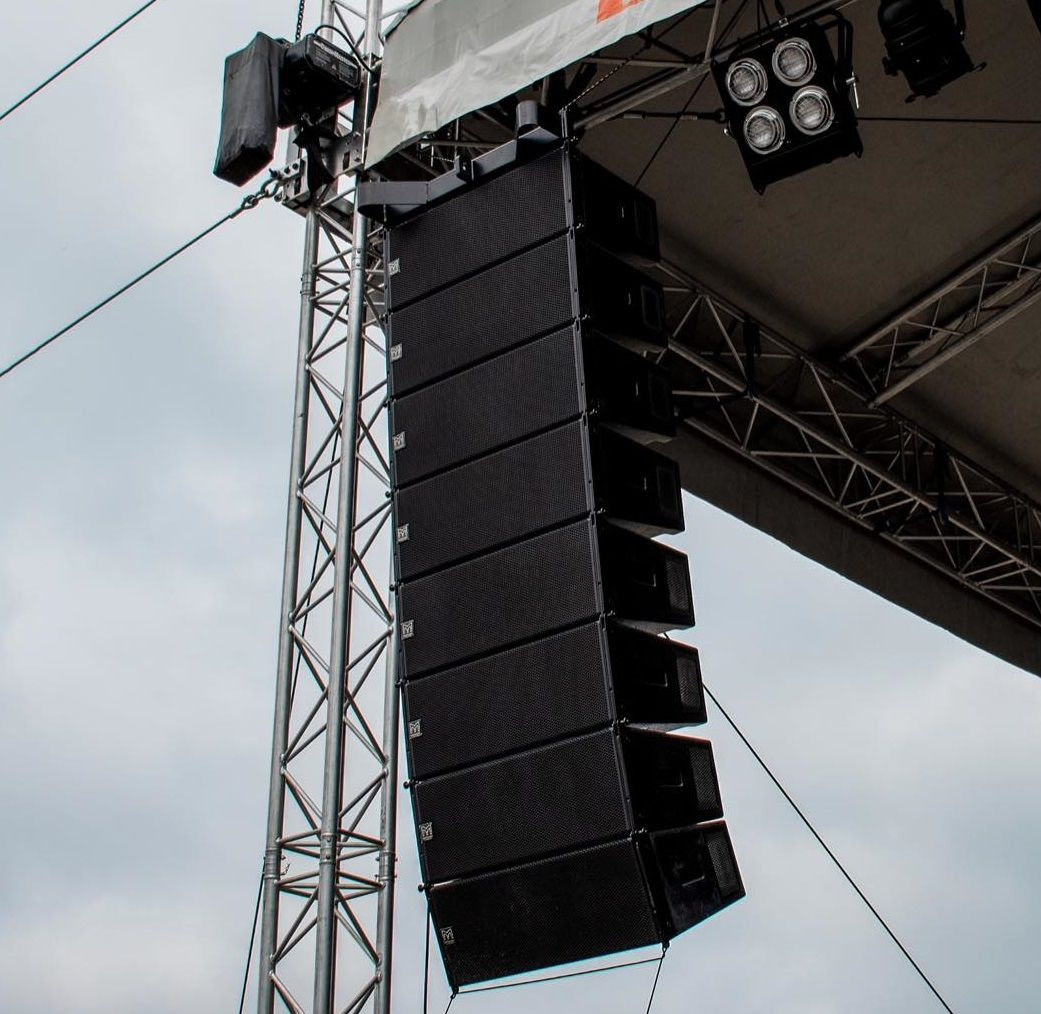
\includegraphics[width=150px, keepaspectratio]{figures/line_array.jpg}
		\caption{Line Array rendszer}
        \label{fig:line_array}
	\end{minipage}
\end{figure}
%----------------------------------------------------------------------------
A Line Array rendszerek ezzel szemben több szegmensből állnak, amelyek egymáshoz képest függőlegesen vannak elrendezve.
Minden láda több-kisebb hangszórót tartalmaz. Amikor ezek a komponensek sorba vannak állítva, 
együtt működnek egy hatékony és kontrollált hangzás előállításában, amely sokkal könnyebben irányítható. 
A Line Array rendszerek ideálisak nagyobb eseményekhez vagy szabadtéri koncertekhez, mivel képesek 
nagyobb területet lefedni. Az ilyen rendszerek vezérlése lehetővé 
teszi olyan okos megoldások alkalmazását is, mint például a \textit{kizárási zónák} létrehozása, vagy a 
hang egy adott területre való fókuszálása a helyszínen.
Összefoglalva, a pontsugárzó és a Line Array hangszórók közötti alapvető különbség a hangterjesztés módjában rejlik. 
Míg a pontsugárzó hangszórók a hangot minden irányba szórják, addig a Line Array hangszórók a hangot meghatározott területekre irányítják. 
A pontsugárzók inkább kisebb rendezvényekhez ajánlottak, míg a Line Array rendszerek nagyobb helyszínekhez vagy szabadtéri eseményekhez ideálisak.
%----------------------------------------------------------------------------
\subsection{LineArray DSP-vezérelt irányítás~\cite{AHNERT2023}}
%----------------------------------------------------------------------------
A hangosító rendszerek tervezésének fő célja, hogy a közönség számára kiváló minőségű hangzást biztosítson. 
A kiváló hangzás alatt egyenletes hangerejű, homogén frekvenciaválaszú, alacsony torzítással rendelkező és mindenhol jól érthető hangot értünk. 
E célok elérése érdekében a modern lesugárzó rendszerek elektronikus úton állítható irányokkal rendelkeznek. 
Ehhez egyedi digitális jelkezelést (DSP) és egyedi erősítést alkalmaznak minden egyes meghajtóhoz.
%----------------------------------------------------------------------------
\begin{figure}[H]
    \centering
    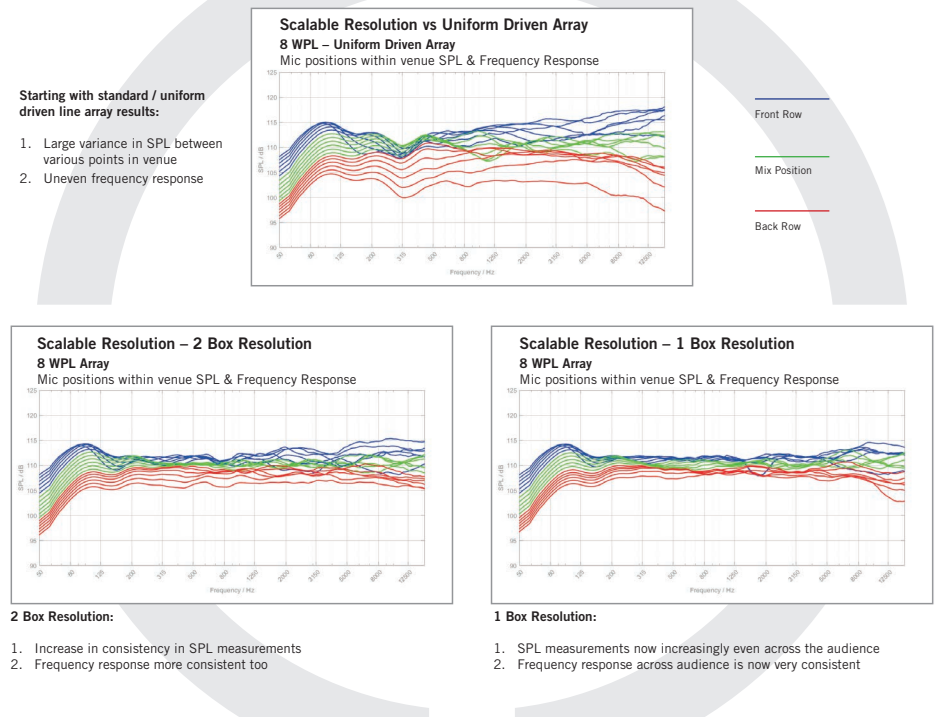
\includegraphics[width=350px, keepaspectratio]{figures/dsp_arrays.png}
    \caption{DSP-vezérelt Line Array~\cite{AHNERT2023}}
    \label{fig:dsp_arrays}
\end{figure}
%----------------------------------------------------------------------------
A DSP-vezérelt line array hangszórók találmánya az 1990-es évekre nyúlik vissza, és azóta folyamatosan fejlődik.
Ma már számos gyártó kínál különböző méretű és felbontású DSP-vezérelt irányítható rendszereket, 
amelyek igyekeznek minden hangosítási igényt kielégíti. 
Különösen akusztikailag nehéz helyszíneken, ahol sok a reflektáló felület és nagy a visszhang effektus. 
Itt az ilyen vezérléssel rendelkező rendszerek teljesítménye egyértelműen felülmúlja a hagyományosak eredményeit. 
A DSP programozása speciális szoftvert igényel, amelyet a gyártó biztosít, és lehetővé tesz különböző szűrő paraméterek optimalizálását a kívánt irányítottság eléréséhez. 
Általában a cél egy keresztmetszeti tervként van meghatározva, és a line array rendszer irányítása ennek a célzott terület egyenletes lefedésére irányul.
A rendszerek tervezése számítógépes eszközöket igényel, amelyek lehetővé teszik a hangszórók viselkedésének részletes szimulációját, például hogyan reagál a térben egy bizonyos rendszer.

\begin{comment}
Ha még szükség van oldalszámra, a bevezető részben talán érdemes lenne részletesebben írni a hangszórókról, 
esetleg egy kis teremakusztikáról is (milyen hangszóróelrendezés hogyan befolyásolja a hangzást, miért előnyösebb vagy hátrányosabb a line array stb.).
\end{comment}
%----------------------------------------------------------------------------
\chapter{\AudioOverIp}
%----------------------------------------------------------------------------
\section{Bevezetés az Audio over IP világába}
%----------------------------------------------------------------------------
A 90-es évek vége óta a szakmai hangipar elmozdult a pont-pont digitális
átviteli formátumoktól (például AES/EBU vagy MADI) az IP-alapú szabványok felé
(például AES67). Ez a csomag alapú hálózati megoldás hatalmas rugalmasságot
hozott, valamint kibővített vezérlési és monitorozási képességeket biztosít
hangrendszerek számára. Lehetőséget teremt arra, hogy egy fizikailag már meglévő
telepítés későbbi szoftverkonfigurációval és frissítésekkel alkalmazkodóvá és
bővíthetővé váljon. A gyártó különböző esetekben akár teljesen új funkciókkal is
kiegészítheti a már meglévő eszközöket. 
A jelutak az IP alapú megközelítés miatt már nem kötődnek 1:1 fizikai kábelekhez, hanem
bármikor pár egérkattintással megváltoztathatóak anélkül, hogy szükség lenne bármilyen
jellegű fizikai átrendezésre, vagy dedikált audio útválasztó hardverre. 
A csomagorientált átvitel jellegéből adódik, hogy az audiojelek automatikusan eljutnak 
a kívánt helyre az IT hálózaton keresztül.
A Cirrus Logic által 1996-ban bevezetett CobraNetet
általában az első sikeres audio-over-ethernet hálózat-implementációnak tekintik,
és számos audio telepítés alapját képezi. Ezek közé tartoznak különböző kongresszusi központok,
színházak, koncerttermek, repülőterek és vidámparkok.
Bár ma is sok CobraNet telepítés létezik, magas késleltetési problémák és korlátozott mérethatékonyság
miatt nem ideális élő hang, stúdiófelvételek és rádió létesítmények számára.
A mintegy tíz évvel később megjelent egy ausztrál cég az Audinate, és az általuk kifejlesztett
Dante a `Digital Audio Network Through Ethernet'. Dante több jelentős
előnnyel rendelkezik az első generációs audio-over-IP technológiákhoz viszonyítva.
Ezek közé értve a jobb használhatóságot és magasabb kompatibilitást a szabványos
hálózati infrastruktúrával. A Dante egy hatalmas hardveres ökoszisztémából
profitál, több száz gyártó által gyártott ezernél is több eszközzel. 
Mielőtt a Dante elérte volna jelenlegi domináns pozícióját, nagy várakozás volt egy AVB
(Audio Video Bridging) nevű technológia körül.
Más iparágak, például az autóipar és az ipari automatizálás, átvették az AVB-t, és
általánosabb nevet adtak neki, mivel az már nem csak hang és videóalkalmazásokhoz kapcsolódik.
Az AVB-t a gyártók fejlesztőcsoportja, az AVnu Alliance időérzékeny hálózat (TSN) néven nevezte el.
Később a Milan munkacsoport, egy audio/video gyártókból álló konzorcium, úgy
döntött, hogy kidolgoz egy finomhangolt specifikációt a profi audio/video
rendszerekben való használatra, Milan néven. 
Ez egy specifikus TSN verzió, amely az audio/video szolgáltatók közötti interoperabilitásra összpontosít.
Ez nem a TSN alapján történt, mivel a TSN-hez speciális IT hardver szükséges az audio
követelmények kezeléséhez, és csak korlátozott számú kapcsolómodell támogatja a TSN-t. 
%----------------------------------------------------------------------------
Az átmenet az IP hálózatokra összehasonlítható az analóg hangról a digitális
hangra való átmenettel. Először csak néhány kezdeti telepítés, amelyek az új technológiát
használják, majd esetleg hiányosságokat mutathatnak a kezelés vagy a megbízhatóság
terén a hagyományos régi megközelítéshez képest, de ezek idővel a technológia fejlődésével eltűnnek. 
Vannak területek, ahol az IT hálózatok alapvetően más módon működnek, mint a hagyományos audio útválasztás.
Először is, egy szabványos IT hálózat nincs kialakítva szigorú időzítési követelmények
teljesítésére, amelyek általában az audio esetében jellemzőek. 
Egy hálózati környezetben az adatcsomagok útját más csomagok is akadályozhatják, ami jelentős
időbeli változást eredményezhet az érkezési időben.
A hagyományos audio kábelek esetében az adatok továbbításának időzítése nem változott meg a kábel által.
Másodszor, egy csomag elvesztése elfogadhatónak tűnhet és tűnik a szokásos IT
alkalmazások esetében, mivel azok automatikusan újraküldésre kerülnek, ha elvesznek.
Az audio alkalmazások esetében a késleltetés minimalizálása érdekében
létfontosságú, hogy a csomagok az első alkalommal a korrekt helyre érkezzenek meg, mivel egyáltalán nincs
elegendő idő az újraküldéshez. Ha néhány csomag elveszik, az azonnal hallható megszakításokat és kimaradásokat okoz.
A csomagvesztés gyakori oka a linkek túlterhelése, vagy a túl alacsony pufferméret.
Az audiohálózatokat oly módon kell kialakítani, hogy elegendő sávszélesség álljon rendelkezésre
minden felhasználójuk számára. Ha ez teljesül, és a csomagkiszállítás időben történik, ahogyan az audio alkalmazások igénylik,
akkor a hálózatunk már elméletileg képes stabilan működni.
Érdemes túlbiztosítani a hálózatot oly mértékben, hogy minden csomag időben
megérkezzen, anélkül, hogy további finomításra lenne szükség a kapcsolók
konfigurációjában. Konkrétan ez azt jelenti, hogy olyan IT hálózatokat kell
építeni elegendő sávszélességgel, és kizárólag az audio alkalmazások számára
kell használni, tehát ne keveredjenek általános mindennapi alkalmazásokkal. 
%----------------------------------------------------------------------------
A legtöbb audio-over-IP technológia abból indul ki, hogy az alapul szolgáló
hálózat megfelelően fog működni. Gondolva itt arra, hogy nincsen csomagvesztés, 
nincs súlyos ütközés más csomagokkal a kapcsoló hardveren. 
Néhány hálózatban, különösen ha az audio és más forgalmat keverik, 
fontos lehet az audio és szinkronizációs csomagoknak elsőbbséget biztosítani másokkal szemben,
például az internetes böngészéssel szemben. Ez a mai legtöbb kereskedelmi forgalmazott
kapcsolóval elérhető. 
Példa audio over IP hálózatokra:
%----------------------------------------------------------------------------
\begin{itemize}
	\item Audinate által kifejlesztett Dante
\end{itemize}
\begin{itemize}
	\item QSC által kifejlesztett Q-LAN
\end{itemize}
\begin{itemize}
	\item Lawo és Partnerei által kifejlesztett RAVENNA
\end{itemize}
%----------------------------------------------------------------------------
\begin{figure}[H]
	\centering
	
\includegraphics[width=60mm, keepaspectratio]{figures/dante_logo.jpg}
	\caption{Audinate Dante logó}
	\label {fig:dante_logo}
\end{figure}
%----------------------------------------------------------------------------
\subsection{Előnyök és hátrányok}
%----------------------------------------------------------------------------
Az IT hálózatok alkalmazása hangkapcsolatokra nézve számos előnyt kínál:
\begin{itemize}
	\item Rugalmasság a hangkapcsolatok hozzáadásához vagy módosításához anélkül,
	      hogy a kábeleket cserélnénk.
\end{itemize}
\begin{itemize}
	\item Az IT viszonylag alacsony áron széles skálájú funkciót kínál.
\end{itemize}
\begin{itemize}
	\item Az alkalmazkodás és integráció az IT hálózati infrastruktúrába
	      specifikus audio vagy videokábelek alkalmazása nélkül.
\end{itemize}
\begin{itemize}
	\item Videójel és vezérlési adatok továbbíthatók ugyanazon infrastruktúrán
	      keresztül.
\end{itemize}
%----------------------------------------------------------------------------
Ugyanakkor az audio-over-IP hálózatok felhasználóit számos kihívás elé is állíthatják:
%----------------------------------------------------------------------------
\begin{itemize}
	\item Azért mert általában több hangmintát egy csatornából egy csomagba helyeznek
	      el a hatékonyság érdekében, adott minimális késleltetés adódik, mivel az
	      küldőnek meg kell várnia, hogy a hangminták rendelkezésre álljanak, mielőtt
	      azokat átküldené a hálózaton. Ez a késleltetés általában magasabb, mint a
	      pont-pont digitális hangszabványok esetében, de optimalizált csomagformátumok és
	      hálózati beállítások segítségével minimalizálható és nagyon jól közelíthető.
\end{itemize}
\begin{itemize}
	\item Mivel az IT hálózatok nem meghatározottak a csomagok úti idejét tekintve,
	      egy biztonsági tartományt, azaz egy audio buffer-t kell beszúrni a fogadó végén.
	      Ez a buffer további késleltetést eredményez. Minél kevesebb csomagütközés van
	      jelen a hálózatban, annál inkább csökkenthető ez a biztonsági tartomány (és
	      ezzel a késleltetés).
\end{itemize}
\begin{itemize}
	\item Az audio csomagformátumok változatossága miatt növekszik a komplexitás,
	      ami azt jelenti, hogy a fogadóknak és küldőknek azonos beállításokkal kell
	      rendelkezniük. Az audio-over-IP technológia komplexitása jelentősen magasabb,
	      mint az előző technológiáké. Az iparág még mindig jelentős munkát végez annak
	      érdekében, hogy csökkentse ezt a komplexitást a felhasználó számára, bevezetve
	      intelligens és felhasználóbarát szoftvermegoldásokat az audiohálózatok
	      kezelésére.
\end{itemize}
%----------------------------------------------------------------------------
\subsection{Fázishelyesség}
%----------------------------------------------------------------------------
A legtöbb audio alkalmazásban kritikus a több eszköz szinkronizált viselkedése.
Elengedhetetlen a mikrofonok vagy hangszórók közötti fázispontosság.
Amikor több hangszóró van csatlakoztatva egy erősítőhöz, és az összes csatorna
egyetlen hangcsomagban érkezik meg, nincs veszélye annak, hogy a csatornák
ellenfázisban lennének egymással, mivel a hangminták nem változhatnak el egymás
között a hálózaton keresztüli átvitel során. 
Azonban egyre több alkalmazásban több erősítő és processzor függetlenül kap hangcsomagokat,
miközben továbbra is szükség van arra, hogy pontosan reprodukálják az audiojeleket egyező fázispontossággal.
Ezért egy adott audio csomagot több hálózati eszköz is megkaphatja, pufferelheti, és ezeket
pontosan ugyanabban az időben kell lejátszania. 
Mivel nincsenek szoros időzítési specifikációk az IT hálózatokban a csomagok továbbításának és
megérkezésének időpontjára vonatkozóan, az audiohálózatoknak mindenképpen szinkronizációs
módszert kell biztosítaniuk. Ez egy fontos, de új probléma a hálózatokban, amellyel az összes
audio-over-IP technológiának foglalkoznia kell.
Az audiohálózaton belül minden eszköz abszolút időben szinkronizált
a Precision Time Protocol (PTP) szerint. Ez azt jelenti, hogy belső óráik (PTP
követők) egy referenciaóra eszközből (PTP vezető) származnak. Ez az eszköz
bármilyen audioeszköz lehet, amely biztosítja ezt a funkciót, vagy akár egy
speciálisan erre a célra kifejlesztett termék is lehet a pontos PTP órák előállítására.
A vezetőt egy felhasználói beállítás vagy alternatívaként egy szabványos
automatizmus választja ki. Az összes eszköz számára, legyen az audio adó vagy
vevő, az a végső követelmény, hogy pontosan szinkronizálódjanak ehhez az adott időhöz.
Az audio csomag küldési pillanatában egy időbélyegzővel látják el. A felhasználó állandó időeltolást állít be az
összes vevőnél, ez a linkeltolás. Amikor egy csomag megérkezik egy vevőhöz, a
pufferben marad, amíg lejátszásra kerül. Tehát az audio lejátszás pillanata a
küldési idő plusz a linkeltolás. Minden vevő két feltétel mellett érheti el egymás
között a fázispontosságot: 
Pontos időszinkronizálás a PTP óra vezetőjéhez (azonos időbázis) 
Azonos linkeltolási érték beállítása a felhasználó által az összes vevőeszközön
Ezért a linkeltolást az érintett összes kapcsolat legrosszabb esetű késleltetése alapján kell kiválasztani. 
Javasolt bizonyos engedményt hozzáadni az esetleges csomagkiszállítási idők váratlan eltéréseinek esetére,
ez azt jelenti, hogy kicsivel nagyobb időt hagyunk az átlagos csomagfeldolgozási időnél.
Szerencsére ez a koncepció elterjedt és jelenleg minden audiohálózati szabványban és a videóban is használatos. 
%----------------------------------------------------------------------------
\begin{figure}[H]
	\centering
	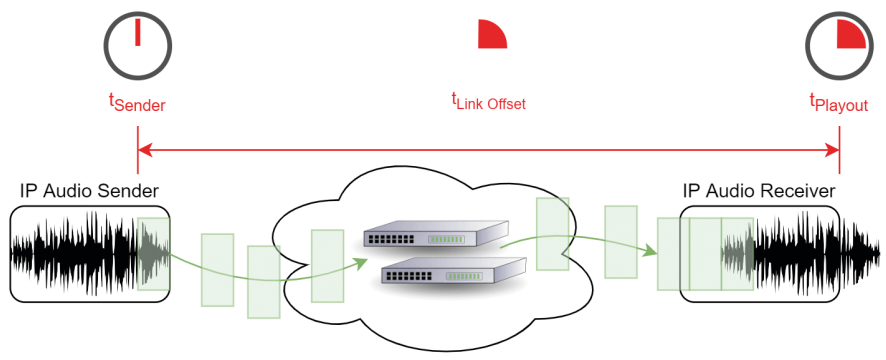
\includegraphics[width=\linewidth, keepaspectratio]{figures/link_offset_latency.png}
	\caption{A kapcsolati eltolás meghatározza a késleltetést \cite{AHNERT2023}}
	\label {fig:link_offset_latency}
\end{figure}
%----------------------------------------------------------------------------
\begin{figure}[H]
	\centering
	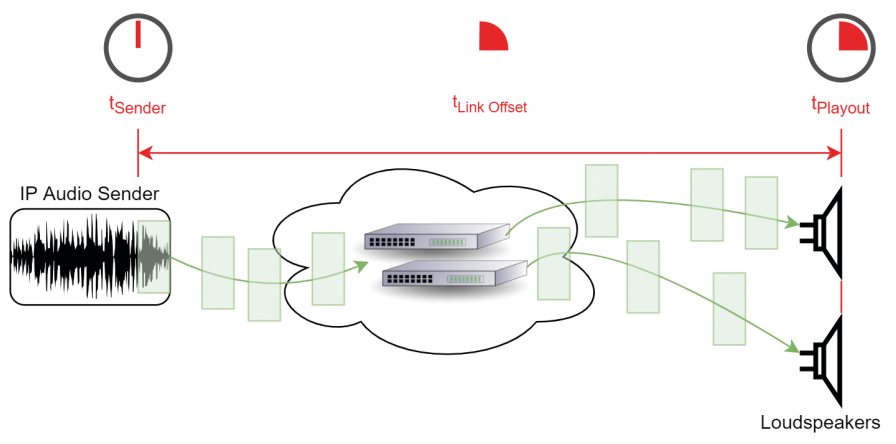
\includegraphics[width=\linewidth, keepaspectratio]{figures/phase_coherence_link_offset.png}
	\caption{Fáziskoherencia azonos kapcsolati eltolással \cite{AHNERT2023}}
	\label {fig:phase_coherence_link_offset}
\end{figure}
%----------------------------------------------------------------------------
\subsection{Szinkronizáció}
%----------------------------------------------------------------------------
Az IP küldők és fogadók szinkronizációja az alacsony késleltetéssel való szinkronban lévő működéshez elengedhetetlen.
A hagyományos audio technológiákban az eszközöket vagy külön \textit{word clock} kapcsolattal, 
vagy szinkronizált audio formátumokkal, például AES/EBU vagy MADI segítségével szinkronizálták.
A fogadók közvetlenül képesek voltak azokból az formátumokból frekvenciájukat és fázisukat kinyerni,
mivel valamiféle \textit{impulzust} biztosítottak, ami jelzi a pillanatot, amikor egy
audio minta létrejön vagy lejátszódik, például analóg-digitális konverterek esetében.
Az PTP csomagok kicsik és nem tartják fel a forgalmat sokáig, de fontos, hogy a
kapcsolókban a lehető legmagasabb prioritással továbbítsák őket. 
Ez végül növelni fogja a szinkronizáció pontosságát. 
A QoS-hez (Quality of service) kapcsolódóan ez azt jelenti, hogy a PTP csomagokat még a hangnál is magasabb prioritással kell
kezelni. Az összes hálózati eszközt ugyanazon naptári időpontra szinkronizálják a Precision Time Protocol
(PTP) segítségével. Ennek az időnek a kiindulása egy olyan eszköz, amelyet óraleadernek
neveznek, míg az ehhez igazodó eszközöket óra követőknek hívják. 
Minden eszköznek meg kell hozzá generálnia a kívánt hagyományos órát (például 96 kHz), amelyet a PTP-n keresztül kapott
abszolút időből származtat. Ez a belső óra a \textit{médiaóra}. 
Ha a gyártó megfelelően implementálja, minden eszköz médiaórájának pontosan ugyan annyinak kell lennie a
frekvencia és fázis terén. A magas pontosság technikailag elérhető, de kihívást
jelent az audio gyártók számára. Ezért a PTP szinkronizált eszközök közötti
fázispontosság minőségtől függően változhat. Elfogadható változásnak tekinthető ha az kisebb mint <1 µs, azaz 1 mikroszekundum.
%----------------------------------------------------------------------------
Mivel az IT hálózatok nem eléggé determinisztikusak a csomag kézbesítésének időpontját
illetően, a készülékek pontos szinkronizációja kifinomult megközelítést igényel.
A PTP követők fő feladata két hatás kompenzálása, amelyek bármilyen hálózat esetén előfordulhatnak:
%----------------------------------------------------------------------------
\subsubsection{Jitter kompenzáció}
%----------------------------------------------------------------------------
A PTP vezető által a szinkronizációs üzenetekben megadott jelenlegi időt az összes követőnek egy jól ismert multicast
cím (224.0.1.129) használatával mutatják be. 
A hálózat és a kapcsolók sorai természetükből adódóan ez az információ nem mindig érkezik meg állandó
késleltetéssel a vevő számára. 
Ez a változás a csomag jitter vagy csomag késleltetési változás (PDV) néven ismert effektus,
ezt az elváltozást minden PTP követőnek kompenzálnia kell. 
Általában az audio hálózatok 1--8 üzenet/mp szinkronizálási arányt
használnak. (A 8-as maximális érték csak kompatibilitás érdekében javasolt)
%----------------------------------------------------------------------------
\subsubsection{Késleltetés mérése}
%----------------------------------------------------------------------------
A követő második kulcsfontosságú feladat a vezető és a követő közötti
csomagkésleltetés mérése a vezető által a szinkronizációs üzenetekben kapott
idő kijavításához. Ehhez szükség van arra az időmérésre, amelyek azt mutatja meg számunkra,
hogy a hálózati út során mennyi időbe telik egy csomag átvitele.
Ez a mérés magában foglalja az összes közöttük lévő
összetevő késleltetését, beleértve a kábeleket és kapcsolókat is. 
A vezető és a követő közötti kábelhossz és a kapcsolók száma nem számít, csak a végső érték.
A PTP időnek az összes követő között ugyanannak kell lennie nanoszekundum pontossággal.
Az egyetlen feltétel a PTP számára, hogy a késleltetés mindkét irányban, a vezetőtől a
követőig és fordítva, állandó és szimmetrikus maradjon.
A késleltetést a követő két üzenet cseréjével méri, a késleltetési kérésből és a késleltetési válaszból következően.
Ezt a késleltetést általában a szinkronizálási aránnyal azonos gyakorisággal hajtják végre, 
azaz az előbbiekben már említett 1 és 8 alkalom között.
Mivel egy vezetőnek minden egyes követővel üzenetet kell cserélnie, van egy maximális követőszámra
vonatkozó korlátja. Sajnálatos módon ez nincs egyértelműen meghatározva, mivel
ez az érték a használt üzenetsebességektől függ.
%----------------------------------------------------------------------------
Mivel a hálózaton több eszköz is képes lehet PTP vezetőként működni és elosztani
az időt az összes követőnek, a szabvány szabályokat hozott létre a vezető
kiválasztásához. Ezt a szabályt a Best Master Clock Algorithm (BMCA), vagyis a
Legjobb Mesteróra Algoritmusnak nevezik. Minden vezetőképes eszköz küldhet
bejelentő üzeneteket a prioritásairól (amelyeket a felhasználó állít be),
valamint az oszcillátor pontosságáról. Ezenkívül figyelnie kell más eszközöket,
amelyek szintén elküldhetik saját bejelentő üzeneteiket. 
Ha más bejövő üzenetek jobb minőséget jelentenek, az eszköz leállítja a vezetőként való bejelentkezését.
Ellenkező esetben rendszeresen küldi saját üzeneteit, mintegy \textit{szívverésként},
és ezzel jelezve minden másik eszköznek az aktív állapotát. 
Ezeket az üzeneteket az announce intervallumnak nevezett időközönként küldik el. 
A bejelentő üzenetek szolgálnak \textit{szívverésként} is, hogy mások tudják, a jelenlegi mester még működőképes.
Ha a kapcsolat megszakad, az összes egység vár egy bizonyos időt (bejelentő időtúllépés),
amíg elküldik bejelentő üzeneteiket, majd megismétlik a kiválasztási folyamatot. 
A vezetőváltás idején a követőknek folytatniuk kell saját oszcillátoruk belső működését.
Az audio nem szakítható meg a vezetőváltás során.
A bejelentő üzenetekben megadott minőség két értéket tartalmaz, amelyeket a felhasználó állít be: prioritás 1 és prioritás 2.
Mindkettő értéke 0 és 255 között változhat, ahol az 0 a legjobb és legyőzi a többieket.
Ha egy prioritás 1 érték kisebb egy eszközön, mint más eszközökön,
akkor az lesz a vezető. A prioritás 2 alatti érték csak akkor releváns, ha
minden előző érték, beleértve a prioritás 1-et is, több eszközön ugyanaz. 
Ez előfordulhat két azonos típusú eszköz telepítéseknél, amelyeknek a felhasználó
azonos értéket állított be a prioritás 1-hez. Ebben az esetben a prioritás 2
határozza meg, hogy melyik lesz a fő vezető, és melyik a tartalék. 
Fontos megjegyezni, hogy néhány eszköz nem kínál lehetőséget a felhasználónak ezen értékének megadására.
Ehelyett egyszerűen a \textit{Preferált Vezető} megjelölésével rendelkeznek.
Technikailag ezek a termékek rögzített értéket használnak bejelentő üzeneteikben, amit a gyártó határoz meg.
Ezért még mindig lehetséges, hogy egy másik PTP vezetőnél beírva egy még alacsonyabb értéket, felül bírálhatja az ilyen típusú eszközt.
Néhány eszköz támogatja azt a beállítást is, amit \textit{Csak Követő} néven ismerünk. Ebben az esetben amikor ez engedélyezve van,
az adott eszköz sosem próbálja meg átvenni a vezetői szerepet az PTP hálózaton.
%----------------------------------------------------------------------------
\subsection{Mintavételi frekvencia és bitmélység}
%----------------------------------------------------------------------------
Az audio over IP rendszereknél a kifogástalan működéshez elengedhetetlen a számunkra
megfelelő mintavételi frekvencia és bitmélység meghatározása.

Ezek a paraméterek alapvetően befolyásolják az audio minőségét és a hálózati teljesítményt.
Fontos figyelembe venni az átviteli kapacitást, valamint az egyes eszközök maximális mintavételi frekvenciáját és bitmélységét.
Amennyiben a hálózat nem képes a megfelelő sávszélesség biztosítására, a hálózatunk instabillá válhat, 
hangkimaradások és megszakadások, legrosszabb esetben a hálózat összeomlása is előfordulhat.
A gyakran alkalmazott 48 kHz-es mintavételi frekvencia széles hangsávot biztosít, és kompatibilis a legtöbb
professzionális hangtechnikai alkalmazással. 
Nemrégiben kezdett el jobban elterjedni szélesebb körben is a 96 kHz-es mintavételi frekvencia, ami
nagyobb részletességet és jobb hangminőséget eredményez, de cserébe nagyobb sávszélességet igényel.
A sávszélesség kiszámítása a következő képlettel történik:
%----------------------------------------------------------------------------
\begin{equation}
	\label{eq:sávszélesség}
	Sávszélesség igény = MintavételiFrekvencia * BitMélység * CsatornákSzáma
\end{equation}
%----------------------------------------------------------------------------
Ezzel a formulával könnyen és gyorsan kiszámíthatjuk, hogy a rendszerünknek mekkora sávszélességre lesz szüksége.
Tehát ha egy 64x64 csatornás rendszerünk van, 96 kHz-es mintavételi frekvenciával és 24 bites bitmélységgel,
akkor a sávszélességünk a következő lesz:
%----------------------------------------------------------------------------
\begin{equation}
	\label{eq:sávszélesség}
	96000 * 24 * 64 * 2 = 294912000 bit/s = 294,912 Mbit/s (nyers adatfolyam)
\end{equation}
%----------------------------------------------------------------------------
Mivel a hálózatunkat a Dante által ajánlott méretezés szerint szeretnénk kialakítani,
legalább 30 százalékos túlméretezést kell alkalmaznunk. Tehát a fenti példában a sávszélességünk a következő lesz:
%----------------------------------------------------------------------------
\begin{equation}
	\label{eq:teljes-sávszélesség}
	294912000 bit/s * 1.3 = 383385600 bit/s = 383,3856 Mbit/s (teljes sávszélesség)
\end{equation}
%----------------------------------------------------------------------------
A számítások alapján egy átlagos 1 Gbit/s (1 Gbit/s = 1000 Mbit/s) sávszélességű hálózaton ez a rendszer már megfelelően működhet.
Érdemes a hálózatunkat túlbiztosítani, hogy a rendszerünk a legnagyobb terhelés alatt is megfelelően működjön.
A bitmélység a hangsáv digitális reprezentációját határozza meg, és az adatok pontosságát befolyásolja.
Általában 16 vagy 24 bitmélységű rendszerek használatosak az audio over IP területén, de a Dante rendszerek a 
32 bites bitmélységet is támogatják. A 16 bites reprezentáció megfelelő lehet olyan alkalmazásokhoz, ahol a nagy
dinamikatartomány nem kritikus. Ugyanakkor a 24 bites felbontás lehetőséget nyújt a pontosabb és részletesebb hangátvitelhez,
általában zenei stúdiókban és élőzenei környezetekben. 
A 32 bites bitmélység a legmagasabb minőséget biztosítja, de a sokkal nagyobb sávszélesség igénye miatt elsősorban csak
a kiemelten professzionális stúdiókban használják.
%----------------------------------------------------------------------------
\subsection{Késleltetés}
%----------------------------------------------------------------------------
Amennyiben egy csomag például 1 ms (milliszekundum) hanganyagot tartalmaz, a kapcsolat
késleltetése mindig nagyobb lesz, mint 1 ms.
A küldőnek először 1 ms hangot kell pufferelnie, mielőtt beleteszi egy csomagba, majd elküldi a hálózaton.
Ezt követi a hálózaton történő utazás ideje az összes kapcsolóval, mielőtt végül eljutna a fogadó eszköz pufferébe.
%----------------------------------------------------------------------------
\begin{enumerate}
    \item Csomag idő
    \item Utazási idő a hálózaton
    \item Fogadási puffer
\end{enumerate}
%----------------------------------------------------------------------------
A gyakorlatban a link offset technikai kifejezés egyenlő a késleltetés fogalmával.
A felhasználó felelőssége, hogy olyan link offsetet válasszon, amely elég hosszú, hogy a fogadó puffer soha ne ürüljön ki, és
ezáltal soha ne történjen meg a hang megszakítása. 
%----------------------------------------------------------------------------
\subsection{IP címek és maszkok}
%----------------------------------------------------------------------------
Egy hálózaton belül minden eszköznek egyedi címre van szüksége annak érdekében,
hogy a csomagok sikeresen elérjék a céljukat és elkerüljük a csomagok ütközését.
Egy ilyen cím lehet hardverrel kapcsolatos (MAC-cím) vagy konfigurálható a cím (IP-cím).
%----------------------------------------------------------------------------
\section{IP-cím hozzárendelési módszerek}
%----------------------------------------------------------------------------
Az IP-címeket háromféleképpen lehet hozzárendelni egy eszközhöz:
%----------------------------------------------------------------------------
\begin{itemize}
    \item \textbf{Felhasználói kézi beállítás:}
    Ez dokumentációt és felhasználói fegyelmet igényel annak érdekében,
	hogy egy adott IP-címet csak egyszer használjanak ugyanabban a hálózatban.
	Ez lehet a preferált megközelítés állandó telepítések esetén,
	mivel lehetővé teszi az IP-címek rendelésének bizonyos struktúrájának követését.
    
    \item \textbf{DHCP szerver általi eszközhöz rendelés:}
    Ez egy rugalmas, mégis strukturált módja az IP-címek elosztásának a hálózaton belül.
	Egy hoszt 'DHCP módban' megpróbálja megtalálni a megfelelő DHCP szerveret,
	és minden szükséges IP-konfigurációt egy jól szabványosított módon szerez be.
	Egy felhasználó ellenőrizheti a DHCP szerverben észlelt eszközöket és azok IP-címeit.
	Az adminisztrátor konfigurálhatja úgy, hogy csak bizonyos IP-cím-tartományt osztanak ki,
	míg másokat kézi rendelésre tartalékolnak.
    
    \item \textbf{Hoszt általi önkiosztással:}
    Ez a mechanizmus még \textit{Zeroconfig} néven ismert, és csak kis telepítésnél
	működik a korlátai miatt, mivel az összes eszköz egy alhálózatban van,
	és nem csatlakozhat más alhálózatokhoz.
\end{itemize}
%----------------------------------------------------------------------------
Egy adott eszköz IP-címéről való információ beszerzése alapvetően kissé nehéz lehet,
ha az nem jelenik meg egy kijelzőn. 
Szoftveres eszközök elérhetők az eszközök jelenlétének szkennelésére IP-cím-tartományokban,
de az IT osztályok gyakran tiltják az ilyen eszközök használatát.


Azonosítani, hogy két IP-cím ugyanabba az alhálózatba tartozik-e, nem lehetséges 
a hozzájuk tartozó alhálózati maszkok ellenőrzése nélkül.
Ha egy csomag cél-IP-címe nem ugyanabban az alhálózatban van,
a küldő eszköznek a router IP-címére kell irányítania, ahelyett hogy
közvetlenül a fogadó eszközhöz küldené. 
Két hoszt ugyanabban az alhálózaton belül hasonló IP-címekkel rendelkezik, csak az utolsó számjegyekben
különbözik. Az első részt hálózati címkének nevezik, a másodikat, amely az
eszköz számára egyedi, hosztcímkének. A kettő közötti szétválasztást az
alhálózati maszkban a `0'-s számjegyek pozíciója jelzi.
A hálózati címkét az alhálózati maszkban egy `0'-nál nagyobb érték jelzi,
míg a hosztcím a maradék jobb oldal, ahol az alhálózati maszk `0'-át jelzi.
%----------------------------------------------------------------------------
\begin{figure}[H]
    \centering
    \begin{minipage}{0.45\textwidth}
        \centering
        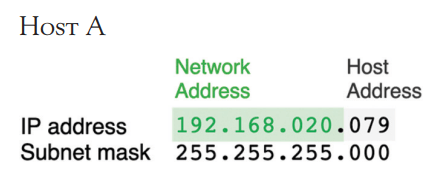
\includegraphics[width=67mm, keepaspectratio]{figures/host_a.png}
        \caption{Host A}
    \end{minipage}\hfill
    \begin{minipage}{0.45\textwidth}
        \centering
        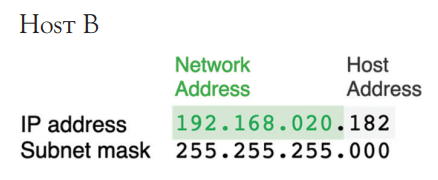
\includegraphics[width=67mm, keepaspectratio]{figures/host_b.png}
        \caption{Host B}
    \end{minipage}
\end{figure}
%----------------------------------------------------------------------------
Host A Host B  Host B ugyanabban az alhálózatban van,
mint Host A, mert mindkettő ugyanazt a hálózati címkét használja (192.168.020).
Az IP-cím hálózati része az a rész, ahol az alhálózati maszk 255-ös értéket
mutat. Ezen két eszköz között egy router nem szükséges. 
%----------------------------------------------------------------------------
\begin{figure}[H]
	\centering
	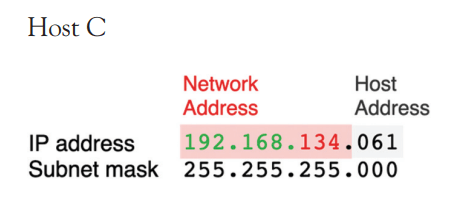
\includegraphics[width=67mm, keepaspectratio]{figures/host_c.png}
	\caption{Host C}
	\label {fig:host_c}
\end{figure}
%----------------------------------------------------------------------------
Host C más alhálózatban van, mint Host A és B, mert különbözik a hálózati címében (192.168.134, nem pedig 192.168.020).
Host C nem tud csomagokat cserélni A és B eszközökkel egy router nélkül. 
Annak érdekében, hogy ez az eszköz kommunikálhasson A és B-vel, más IP-címet kell kapnia,
kezdve a 192.168.134\ldots címmel. 
Vagy más alhálózati maszk is választható az egész beállításhoz,
például 255.255.0.0.
%----------------------------------------------------------------------------
A feljegyzett alhálózati maszkok decimális jelölése dot-decimális jelölésnek nevezik.
Azért, hogy az információt rövidebben jelezzék, gyakran
használt alternatív módszer a CIDR vagy perjeljelölés.
Az IP-cím után azonnal következő perjel után az




alhálózati maszkot a `0'-nál nagyobb értékeket mutatva jelöli meg.
Ez a jelölés az alhálózati maszk bináris formájára utal, tehát a `255' a `11111111' -nek felel meg.
A fenti példákban az alhálózati maszkok tehát bináris formájukban 24
`1'-t tartalmaznak. 
A fenti példában szereplő hosztok CIDR jelölése:
%----------------------------------------------------------------------------
\begin{itemize}
    \item \textbf{Host A:} 192.168.020.182/24
    \item \textbf{Host B:} 192.168.020.079/24
    \item \textbf{Host C:} 192.168.134.61/24
\end{itemize}
%----------------------------------------------------------------------------

A routereket használó és több alhálózatot összekapcsoló telepítések a
az OSI modell 3. rétegén működnek. Ez a modell hét rétegre osztja a
hálózatok általános funkcionalitását, mindegyik egy adott készletet ír le a hálózati
eszközök által nyújtott funkcionalitásokról. Gondolva itt elsősorban a csomagok továbbításáról a
megfelelő címzett felé. Az összes jelenlegi IT eszköz követi ezt a jól
meghatározott absztrakciós rétegkoncepciót, hogy elősegítse a gyártók közötti
interoperabilitást. A 3. rétegen működő telepítések értelmezhetik az IP-címeket,
az alhálózati maszkokat stb., és így továbbítani tudják a csomagokat az
alhálózatok között. Az itt tárgyalt összes technológia képes ilyen
forgatókönyvekben működni. Ezzel szemben néhány technológia korlátozott a 2.
rétegre. Ez azt jelenti, hogy a csomagjaikat kizárólag MAC-címek alapján
szállítják, és nem tartalmaznak alhálózati információkat. Ennek eredményeként a
2. rétegű hálózatokat nem lehet több alhálózatokra bontani, a csomagjaikat nem
lehet routerek által továbbítani, és ezáltal a skálázhatóságuk valamelyest
korlátozott. Az egyik népszerű példa a 2. rétegű hálózatokra a már említett
TSN/Milan, valamint a CobraNet.

%----------------------------------------------------------------------------
\begin{figure}[H]
	\centering
	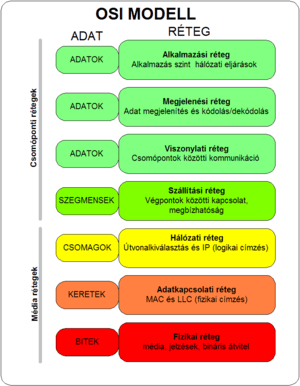
\includegraphics[width=67mm, keepaspectratio]{figures/osi_modell.png}
	\caption{Az OSI modell}
	\label {fig:osi_modell}
\end{figure}
%----------------------------------------------------------------------------

Egy alhálózat egy logikai szegmens egy adott hálózaton belül. Az ilyen szegmenseket
különféle okokból hoznak létre, ideértve elsősorban az adminisztratív és biztonsági
szempontokat. A hálózati adminisztrátor egy készlet szabályt alkalmazhat egy
alhálózatra, míg más szabályokat választhat egy másikra. A routerek képesek
összekapcsolni az alhálózatokat, így a hosztok csomagokat cserélhetnek az
alhálózati határok átlépése nélkül. Egy routernek megfelelően konfigurálva kell
lennie a hálózati útvonalak létrehozásához ezek között az alhálózatok között.
Ezzel szemben egy tipikus kapcsoló nem képes összekapcsolni az alhálózatokat.
Egy virtuális LAN (VLAN) egy másik módszer a hálózat szegmentálására. 
Rugalmasabbá teszi a rendszereket, csökkenti a kapcsolatlan rendszerek közötti fölösleges kommunikációt.
Szemben az alhálózatokkal, ez egy biztonságosabb módja is a hosztok elkülönítésére egymástól.

%----------------------------------------------------------------------------
\subsection{Hálózati topológiák}
%----------------------------------------------------------------------------
A csomópontok különböző módon kapcsolódhatnak össze. A topológia meghatározása
az egyik legfontosabb döntés, amelyet egy hálózat tervezésekor hozni kell. A
csillag topológia sok szempontból a preferált megoldás. Több hoszt egy
útválasztó eszközhöz, például egy kapcsolóhoz vagy routerhez csatlakozik. A mai
hálózatok gyakran két csillagszintet kombinálnak. Ezt gerinc/levél architektúrának
nevezik. A központi kapcsoló/router (gerinc) általában több forgalmat továbbít,
mint a perifériális kapcsoló (levél), mivel a szegmensek közötti legtöbb
forgalom áthaladhat rajta. Ha a gerinc és a levél közötti nagy sávszélességű
kapcsolat nem képes egyszerre továbbítani az összes hoszt forgalmát, akkor ez a
tervezési forma blokkoló. Az ellentéte egy nem blokkoló hálózattervezés, ahol a
nagy sávszélességű kapcsolatok képesek az összes a hozzájuk csatlakoztatott
hoszt teljes forgalmát továbbítani. A gyűrű topológiának több interfésze is lehet:
legalább kettőre van szükség egy gyűrű topológia megvalósításához. Minden két
csomópont közötti kapcsolat teljes sávszélességet kínál, és a csomópontokra
hárul a feladat, hogy továbbítsák a csomagokat a gyűrűn belül. Ebben az
értelemben mindegyik csomópont úgy működik, mint egy kapcsoló, csomagokat
továbbítva két interfésze között. A gyűrű topológia választása gyakran ésszerű,
amikor nagy távolságokat kell áthidalni, és a kapcsolatok költségesek.
Gyakorlati példák a különböző helyszínek közötti hálózatok, de gyűrűket alkotnak
olyan eszközök csatlakoztatására is, amelyek esetében nincs hely egy további
kapcsoló számára. A gyűrű topológiák beépített redundanciát kínálnak minden
eszközhöz hozzáférhetünk, még akkor is, ha egy kapcsolat elszakad.
A megfelelő hálózat kialakításához még elengedhetetlenek a nem blokkoló kapcsolók.
A nem blokkoló architektúra azt jelenti, hogy nem a kapcsoló a szűk keresztmetszet.
Tehát képes kezelni az összes rá táplált forgalmat, csak a port sebessége a korlát.

%----------------------------------------------------------------------------
\subsection{Unicast és Multicast} %Egyedi és Csoportos Küldés
%----------------------------------------------------------------------------

Amikor egy eszköz csomagot küld egy másik eszköznek, ezt unicast mechanizmusnak
nevezzük. Egy ilyen kapcsolatnak pontosan egy küldője és egy fogadója van. Az
unicast gyakran használja a Transmission Control Protocol (TCP)-t, ahol a fogadó
minden egyes csomag sikerült átvételéről visszaigazolást küld a küldőnek. Ha a
visszaigazolás nem érkezik meg, a küldő automatikusan újraküldi a csomagot. 
Az UDP (User Datagram Protocol) egy alternatíva a TCP-nek. Ebben az esetben a küldő
bízik abban, hogy a csomagok sikeresen megérkeznek a fogadóhoz. Nincs
visszaigazolás, és ha a csomag elveszik, a tartalma is elveszik.
Ez az jelenti, hogy az UDP nem annyira megbízható? Valójában nem,
csak egy más eszköz más felhasználásra.
Bár ez váratlan lehet, ez valójában a preferált átviteli mód a szakmai audio hálózatok
számára. Mivel az időkésleltetés alacsonynak kell lennie, nem engedhető meg a
csomagok újraküldése, mert az időt vesz igénybe, és ezzel növelné az általános
időkésleltetést. Az élő audio csomagvesztés esetén a legjobb, ha folytatjuk a
következő audio minták lejátszását, anélkül hogy megpróbálnánk helyreállítani az
előzőt. A menedzselhető switchek és végpontok tudják logolni a csomagvesztéseket, így
monitorozható a hálózat állapota.
Az audio alkalmazásokban gyakran szükség van arra, hogy egy audio jelet
több helyre párhuzamosan fogadjanak, például egy mikrofonjel, amelyet
párhuzamosan továbbítanak a front-of-house és a monitoring keverőpultoknak. Akár
egy harmadik hely is létezhet, például egy felvevő eszköz. 
Amikor a küldő unicast módban továbbítja a csomagokat, az audio jel három csomagként
érkezik azonos tartalommal, de különböző címzési címekkel. Ez felesleges
processzor terhelést jelent a küldő eszköz számára, és emellett sávszélességet
foglal el mindhárom célhoz. Ezt lehet optimalizálni a multicast használatával. 
Számos előnye van, ideértve a küldőre nehezedő kevesebb processzor terhelést 
és az általános forgalom csökkenését a hálózaton. 
A küldő multicast címekre címezi a csomagokat, és nem hoszt címekre. Nem tudja, melyik
címzetteknek érkeznek meg a csomagok. A multicast címek hasonlóak a
rádiófrekvenciákhoz: bárki, aki érdeklődik, bekapcsolhatja és fogadhatja a
tartalmat. A küldő csak egyszer helyezi az audio adatokat egy csomagba, elküldi
egy multicast címre, és a vevőknek tudniuk kell, melyik multicast címre akarnak
hallgatni. A multicast címek alapvetően nem kapcsolódnak alhálózatokhoz, mivel nem
kapcsolódnak a csomópontokhoz és az IP-címekhez. Ezért a multicast csomagok
áthaladnak az alhálózatokon, hacsak nincsenek elkülönítve VLAN-okkal. 
Amennyiben a hálózatunk nem kizárólag az audio jelek továbbítására 
készült speciálisan, néhány eszköz lehet a hálózaton, amelyeknek semmi közük az audiohoz.
Ezért fontos, hogy a multicast forgalom csak
azokhoz a hosztokhoz jusson el, amelyek érdeklődnek iránta. Ennek a megoldása az
IGMP snooping (Internet Csoportkezelési Protokoll). 
Az összes tárgyalt audio hálózati technológia alapértelmezetten
támogatja az IGMP snooping-ot. Ha be van kapcsolva a kapcsolóban, akkor a
multicast-csomagok csak azokon az interfészeken kerülnek elküldésre, ahol a
csatlakoztatott hosztoktól időszakos IGMP kérések érkeznek. Ha nincs beérkező
kérés, akkor a megfelelő multicast leáll, így nem jut felesleges forgalom a
kapcsolaton. Az IGMP snoopingot egyfajta zsilippel lehetne összehasonlítani,
amely alapértelmezetten zárva van, és csak kérésre nyílik meg. Erősen ajánlott
az IGMP snooping bekapcsolása egy multicast hálózatban minden kapcsolóban.
Azonban egy hálózatban csak egy darab IGMP Querier lehet aktív, mivel az
összes többi kapcsoló az aktív IGMP Querier-től kapja az információkat.
Enélkül a multicast úgy viselkedni mint egy broadcast, ami nagy mennyiségű
felesleges forgalmat eredményez.
Összefoglalva, a unicast a legjobb késleltetési teljesítményt nyújtja, és a
kapcsolók számára a legkönnyebben mozgatható.
A multicast pedig jobb sávszélesség-kezelést kínál, ahogy a csatornaszám (és a sávszélesség) nő.

%----------------------------------------------------------------------------
\subsection{Eszköz- és Adatfolyam-felfedezés}
%----------------------------------------------------------------------------

Az AES67 audió szabvány nem határozza meg, hogyan fedezhetik fel egymást a
hálózati eszközök, vagy hogy mely adatfolyamok érhetők el a hálózaton.
Az összes ismert technológia a bonjour vagy mDNS mechanizmust használja eszközeik számára
az egymásról való értesítésre. 
Minden eszköz fix és ismert multicast cím (224.0.0.251) felé küld
üzeneteket, amiket más eszközök elérnek, így értesülnek egymás létezéséről a hálózatban.
Ennek a mechanizmusnak egyik korlátja az, hogy nem működik nagy telepítésekben,
ahol több alcímen vagy VLAN-on vannak. Ezen esetekre a gyártók kifejlesztettek
saját megoldásokat (például Audinate a Dante Domain Manager) vagy
követik az audio/video NMOS szabványt a felismeréshez és kapcsolatkezeléshez.
Az audio adatfolyamokat a gyártótól függően két mechanizmus egyikével fedezik fel. Ahogy
az eszközök felfedezésénél, mindkettő előre meghatározott multicast címet
használ az adatfolyam-információk terjesztésére, hogy a címzettek megtalálják az
elérhető adatfolyamokat és azok paramétereit:

%----------------------------------------------------------------------------
\begin{itemize}
	\item Session Announcement Protocol (SAP) - minden Dante termék által használt (Multicast cím: 239.255.255.255)
\end{itemize}

\begin{itemize}
	\item Bonjour / mDNS - minden más technológiában használt (Multicast cím: 224.0.0.251) 
\end{itemize}
%----------------------------------------------------------------------------
Szerencsére a jelenlegi termékek többsége
lehetővé teszi mindkét protokoll egyidejű aktiválását, így egy adott audio
adatfolyam mindkét mechanizmuson keresztül párhuzamosan bejelenthető.

%----------------------------------------------------------------------------
\subsection{Redundancia}
%----------------------------------------------------------------------------
Az audiohálózatok kezdeti napjaiban egyes felhasználók kételkedtek az IT
hardverek megbízhatóságában. Annak ellenére, hogy a széles körben elterjedt
IT-berendezések jól beváltak és gyakran megbízhatóbbak, mint a hagyományos
audioberendezések. Emellett a legtöbb IT-hálózati komponens több diagnosztikai
mechanizmust kínál a berendezések hibájának gyors felismeréséhez és megoldásához.

%----------------------------------------------------------------------------
\subsubsection{Spanning Tree Protocol (STP)}
%----------------------------------------------------------------------------
Ha a kapcsolókat úgy kötik össze, hogy hurok jön létre, fennáll annak a veszélye, 
hogy a csomagok végtelenül áramlanak a hurokban. 
Ezt az `visszacsatoló hurok' jelenséget a hálózati hardver automatikusan észleli az
STP segítségével, és ha hurokra bukkan, a kapcsoló automatikusan kikapcsol egyik
kapcsolatot. Az STP-t továbbá felhasználhatják a rendszer véletlen
kapcsolatvesztések elleni védelmére is, beleértve a kábelvágásokat is. 

Abból a  megközelítésből áll, hogy szándékosan létrehoznak hurkokat, majd a rendszer
inaktiválja az egyiket. Ha valamelyik kábel véletlenül kiesik, a rendszer
másodperceken belül észleli ezt, és újraaktiválja a passzív kapcsolatot. Ebben
az időszakban az audio néhány másodpercig megszakad, de még mindig sokkal
gyorsabb, mint a manuális hibakeresés és az új kábel telepítése. 
A legtöbb rendszerben az STP alapértelmezetten engedélyezve van. 
Nélküle broadcast 'viharok' alakulnának ki, ami felemészti a sávszélességet.

%----------------------------------------------------------------------------
\subsubsection{Link Aggregáció}
%----------------------------------------------------------------------------
Ha egy adott kapcsolat különösen fontos egy telepítésben, két vagy több kábelt párhuzamosan
lehet csatlakoztatni a biztonság érdekében. 
Bár az ilyen link aggregáció fő célja két kapcsoló közötti sávszélesség növelése, 
ez is költséghatékony módszer lehet egy kapcsolat véletlen leválasztásának
vagy kábelvágásának biztosítására. Tipikus eset például egy színpad, amely egy keverőhöz
csatlakozik. A kapcsolóknak mindkét végén ugyanúgy kell konfigurálni: két vagy
több interfészt kell kijelölni Link Aggregációs Csoportként, és azok
egyetlen interfészként jelennek meg a kapcsolón. Gyakorlatban a linkaggregáció
alkalmazása a kábelproblémák csökkentése érdekében nagyon hasznos lehet
egyszerűsége miatt, hiszen a felhasználónak csak egy további kábelt kell
biztosítania, és azonosítania kell a kapcsolók konfigurációját mindkét végén.
Ugyanakkor a kábelt lekapcsoláskor előfordulhat, hogy az audioátvitel
néhány másodpercig megszakad, mielőtt a kapcsoló alternatív kapcsolatot
aktiválna.
%----------------------------------------------------------------------------
\subsubsection{ Adatfolyam redundancia}
%----------------------------------------------------------------------------
A legbiztonságosabb de egyben legdrágább módja a redundancia megvalósításának
egy hálózatban az, ha két különálló audiohálózatot hoznak létre, 
két független utat biztosítva a küldő és a fogadó között. 
Ebben a felállásban minden csomópontnak két hálózati interfészt
kell biztosítania. A küldő két azonos audio tartalommal rendelkező csomagot hoz létre,
mindkettőre azonos PTP-időbélyegzőt nyom, majd elküldi mindkét hálózaton.
A fogadó végén mindkét csomagot fogadják és kicsomagolják. Még akkor is, ha az egyik csomag
elveszik, a megmaradt csomag tartalmazza az összes információt, és biztosítja,
hogy az audio zavartalanul folytatódik. Valójában ez a mechanizmus az egyetlen
megközelítés egy hálózatban a véletlenszerű csomagvesztés kompenzálására anélkül,
hogy meg kellene ismételni azokat a küldőtől és ezzel késleltetést hozzáadva a rendszerhez.
%----------------------------------------------------------------------------
\section{AES67}
%----------------------------------------------------------------------------
Az AES67 szabvány szerint az összes eszköznek meg kell felelnie az
alábbi minimális specifikációknak: 

%----------------------------------------------------------------------------
\begin{itemize}
	\item Unicast és multicast támogatása
	\item UDP/RTP protokollok használata
	\item DSCP címkék beállítása meghatározott értékekre,QoS támogatás 
	\item Nincs meghatározott automatikus eszköz- és adatfolyam-felfedezés 
	\item PTPv2 szabvány használata az időszinkronizációhoz
	\item PTP profil Standard (a gyakorlatban a Dante jelenleg magasabb szinkronizációs rátát igényel)
	\item Küldőknek ki kell adniuk egy SDP fájlt
	\item A fogadóknak érteniük kell egy SDP fájlt
	\item A fogadó puffernek legalább 3 ms hangot kell tudnia tárolni
	\item Adatfolyam formátumok
	\item Egytől nyolc csatorna (a küldő választhat egy fix számot, de a fogadóknak képesnek kell lenniük rugalmasan fogadni bármelyik lehetőséget).
	\item 24 bites és 16 bites felbontás (a küldő választhat egyet, de a fogadóknak mindkettőt érteniük kell) 
	\item 48 kHz mintavételi frekvencia 1 ms csomagidő (48 minta)
	\item A multicast címek 239.0.0.0 és 239.255.255.255 között vannak 
\end{itemize}


A szabványban sok további paraméter és érték szerepel, de ezek nem szerepelnek a
fent felsorolt minimális követelmények között.

%----------------------------------------------------------------------------
\section{Audinate Dante}
%----------------------------------------------------------------------------
\subsection{A Dante hálózatok áttekintése}
%----------------------------------------------------------------------------
A 2020 - 2021-es Covid-19 járvány alatt lehetőségem volt egy széleskörű átfogó Dante
kurzusra beiratkozni, amelyet a Dante gyártója, az Audinate szervezett. A kurzus
egy átfogó mély áttekintést nyújtott a Dante hálózatokról. Ebben a fejezetben
a fő forrásomnak a belsős oktatóanyagot fogom használni, amelyet a kurzus
során kaptam, pontos és részletes információkat nyújtva a Dante hálózatokról.
Ez a dokumentum csak azok számára elérhető, akik részt vettek a kurzuson.
A Dante hanghálózatok digitális hanghálózati technológiát képviselnek, amely
lehetővé teszi a hang elosztását és útválasztását a szabványos Ethernet
hálózatokon keresztül. Az ausztrál Audinate vállalat fejlesztette ki a Dante-t,
amely a szabványos Internet Protocol (IP) hálózatokat használja a magas minőségű,
alacsony késleltetésű hangátvitelhez eszközök között. Ez lehetővé tesz
nagyobb rugalmasságot és skálázhatóságot a hagyományos analóg hangrendszerekhez
képest, valamint biztosítja a hangrendszer integrálását egy meglévő IT infrastruktúrába.
A Dante hanghálózatokat széles körben alkalmazzák, ideértve a koncerthangosítást,
rádiózást, stúdiófelvételeket, vállalati és konferenciaközpontokat, és még sok mást.
A technológia támogat számos hangformátumot és mintavételi rátát, és lehetővé
teszi akár több száz hangcsatorna egyidejű átvitelét egyetlen hálózaton keresztül.
Emellett a Dante hanghálózatok távolról is vezérelhetők és monitorozhatók,
megkönnyítve a nagy, összetett hangrendszerek beállítását és kezelését.
%----------------------------------------------------------------------------
\begin{figure}[H]
	\centering
	
\includegraphics[width=200px, keepaspectratio]{figures/dante_visual.jpg}
	\caption{Audinate Dante fantázia ábra}
	\label {fig:dante_visual}
\end{figure}
%----------------------------------------------------------------------------

%----------------------------------------------------------------------------
\subsection{Dante hálózatok technikai részletei}
%----------------------------------------------------------------------------
A Dante hanghálózatok két fő komponensből állnak: Dante eszközökből
és Dante hálózatokból. A Dante eszközök olyan hangeszközök, amelyeket
kifejezetten a Dante protokollhoz terveztek, mint például hangkártyák, erősítők
és hangszórók. Ezeket az eszközöket szabványos Ethernet kábelekkel és
kapcsolókkal lehet csatlakoztatni a Dante hálózathoz.
A hálózatot az Audinate Dante Controller szoftverrel lehet
konfigurálni, amely lehetővé teszi a hang elosztását és útválasztását az
eszközök között. A szoftver továbbá lehetővé teszi az eszközök távoli vezérlését
és monitorozását a hálózaton. Ezek a hanghálózatok támogatnak számos
hangformátumot és mintavételi rátát, és képesek egyszerre több száz hangcsatorna
átvitelére egyetlen hálózaton keresztül. A technológia továbbá támogat olyan
fejlett funkciókat, mint a Dante Domain Manager (DDM) a biztonságos
hangátvitelhez, valamint a Dante Virtual Soundcard (DVS) a számítógépes alapú
hanglejátszáshoz és felvételhez. 
Tegyük fel, hogy több eszköz is küld hangot egy adott végpontra a hálózaton.
Alapesetben, ahogy a csomagok felgyülemlenek, az elsőként érkezőket, elsőként szolgálják ki elvet alkalmazzák.
A Dante hanghálózatok Quality of Service (QoS)
támogatást is nyújtanak, a prioritások kezelésére.
Ezzel biztosítható a hangátvitel elsőbbse más hálózati forgalommal szemben. Ez segít minimalizálni a hálózati
torlódás lehetőségét és biztosítani, hogy a hangátvitel minimális késleltetéssel
és magas minőségben történjen. 
Körülbelül 70 százalékos hálózati szaturációnál már ajánlott a QoS használata.
Valamint 100 Mbps-es hálózatoknál segít a jitter csökkenésében.

%----------------------------------------------------------------------------
\subsubsection{Több mintavételi ráta és bitmélység}
%----------------------------------------------------------------------------

A rendszer képes egyidejűleg több bitmélységet kezelni. Ennek informatikai háttere a
a következő képpen néz ki. Ha egy 32 bites hangforrásunk van, de a másik eszköz
csak 24 bites hangot tud fogadni, akkor a Dante a 32 bites hangot 24 bitesre tudja 
alakítani.

%----------------------------------------------------------------------------
\begin{align*}
	\begin{array}{|c|c|}
	\hline
	\text{Hangminták} & \text{Bitmélység} \\
	\hline
	\text{11110000 11110000 11110000 11110000} & \text{32 bites} \\
	\hline
	\text{11110000 11110000 11110000} & \text{24 bites} \\
	\hline
	\end{array}
\end{align*}
%----------------------------------------------------------------------------
	
Amint a példában látszik, 32 bites hangból úgy kaptunk 24 bites hangot, 
hogy egyszerűen csak elhagytuk az utolsó 8 bitet. Ez a folyamat visszafelé is működik,
ha 24 bites hangot kell 32 bites hanggá alakítani, akkor az utolsó 8 bitet 0-val kell feltölteni.

%----------------------------------------------------------------------------	
\begin{align*}
	\begin{array}{|c|c|}
	\hline
	\text{Hangminták} & \text{Bitmélység} \\
	\hline
	\text{11110000 11110000 11110000} & \text{24 bites} \\
	\hline
	\text{11110000 11110000 11110000 00000000} & \text{32 bites} \\
	\hline
	\end{array}
\end{align*}
%----------------------------------------------------------------------------

Mintavételezési frekvencia eltérést csak abban az esetben tudja kezelni, ha a
bitmélység is eltérő. Amennyiben a bitmélység azonos, de a mintavételezési
frekvencia eltérő, akkor a rendszer nem képes a hangot továbbítani.
Ez a mechanizmus egy egyszerű mechanikai példával jól megérhető és leírható.
Tegyük fel van két fogaskerekünk. Amennyiben a mintavételezési frekvencia azonos, és a 
bitmélység eltérő, akkor a fogaskerekek egymásba illeszthetőek és csak a fogaskerekek
mélysége fog eltérni. Amennyiben a mintavételezési frekvencia eltérő, akkor a fogaskerekek
nem illeszthetőek egymásba, és nem tudjuk továbbítani a hangot. Ebben az esetben már egy
konverterre lesz szükségünk, amely képes a két fogaskereket összeilleszteni számunkra.
Egy fontos kitétel van ahhoz, hogy a több mintavételi ráta egyszerre megfelelően működjön,
az pedig az egységes órajel az összes mintavételi frekvenciához.

%----------------------------------------------------------------------------
\subsubsection{Hálózati topológiák}
%----------------------------------------------------------------------------
A Dante rendszerek alapvetően kétféle módban tudnak üzemelni. Az első a
switched (kapcsolt) mód, amelyben az eszközökön található két Ethernet port
egy hálózatot alkot. Ebben a módban tudunk Daisy Chain (füzéres) topológiát kialakítani,
amelyben az egyik eszköz a másikhoz csatlakozik, és így tovább. Továbbá csillagtopológiát
is kialakíthatunk, amelyben minden eszköz egy központi kapcsolóhoz csatlakozik.
%----------------------------------------------------------------------------
\begin{figure}[H]
	\begin{minipage}{0.5\textwidth}
		\centering
		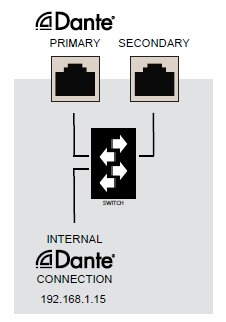
\includegraphics[width=100px, keepaspectratio]{figures/dante-switched-mode.jpg}
		\caption{Kapcsolt mód}
		\label{fig:dante_switched}
	\end{minipage}%
	\begin{minipage}{0.5\textwidth}
		\centering
		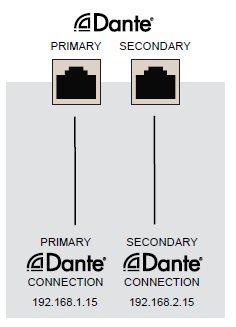
\includegraphics[width=100px, keepaspectratio]{figures/dante-redundant-mode.jpg}
		\caption{Redundáns mód}
		\label{fig:dante_redundant}
	\end{minipage}
\end{figure}

%----------------------------------------------------------------------------
A másik mód a redundant (redundáns) mód, amelyben az eszközökön található két
Ethernet port két különálló hálózatot alkot. Ebben a módban a hálózat redundáns
kialakítású, és a hálózat egyik része automatikusan átveszi a másik rész szerepét,
ha az meghibásodik.
Néhány Dante eszköznek létezik egy harmadik Ethernet portja, amelyet konfigurálási
és vezérlési célokra használnak.
%----------------------------------------------------------------------------
\subsubsection{Késleltetés}
%----------------------------------------------------------------------------
A késleltetés az az idő, amely szükséges a folyamat végrehajtásához. Például
az idő amíg a bemeneti oldalon egy hangjel feldolgozásra kerül, és a kimeneti
oldalon megjelenik. 
Két fő mértékegységet használunk a késleltetés mérésére:
%----------------------------------------------------------------------------
\begin{equation}
	\label{eq:milliseconds}
	1 \text{ másodperc} = 1000 \text{ milli másodperc}, \quad \text{azaz} \quad 1 \text{ ms} = 0.001 \text{ s}
\end{equation}
%----------------------------------------------------------------------------
%----------------------------------------------------------------------------
\begin{equation}
	\label{eq:microseconds}
	1 \text{ másodperc} = 1000000 \text{ mikro másodperc}, \quad \text{azaz} \quad 1 \mu\text{s} = 0.000001 \text{ s}
\end{equation}
%----------------------------------------------------------------------------
A Dante eszközök lehetővé teszik a késleltetés teljesítményének meghatározását. 
A 0.1 milliszekundumos késleltetés az a késleltetés, amely már kapcsoló lépés biztos.
Ha két eszköz különböző késleltetésű, akkor a nagyobb érték lesz az irányadó.
Egy megfelelően konfigurált modern Dante hálózatban a késleltetés 1 ms körüli értéket vesz fel.
Ez azt is jelenti, hogy például egy dobos előbb hallja a hangszerét a fülmonitoron, mint a saját dobját.

%----------------------------------------------------------------------------
\subsubsection{Órajel}
%----------------------------------------------------------------------------

Minden eszköz egy nagyon-nagyon pontos Dátum/Idő órát követ.
Szinkronizálnak az időhöz és állítják a sebességet, hogy egységes legyen.
Mi a helyzet a terjedési késéssel? Miért vannak szinkronban a Dante eszközök?
A PTP (Precision Time Protocol) késleltetési kéréseket (Delay Requests)
ad ki, amelyek kiszámítják a hálózat késleltetését. 
Az eszközök az információváltás késését is kompenzálják.
A Dante automatikusan választ óra vezetőt.
Mindig csak egy óra vezető lesz, függetlenül a mintavételi rátától.
Beállíthatunk külső óra vezetőt is amennyiben szükséges.
Nem szinkronizál újra, hanem beállítja a sebességet és kompenzálja a hálózati késést.
A Dante által végzett tesztelések és tapasztalatok alapján
bebizonyosodott, hogy az időzítés szinkronban marad akkor is,
ha az óra perceken keresztül teljesen eltűnik.

%----------------------------------------------------------------------------
\begin{figure}[H]
	\centering
	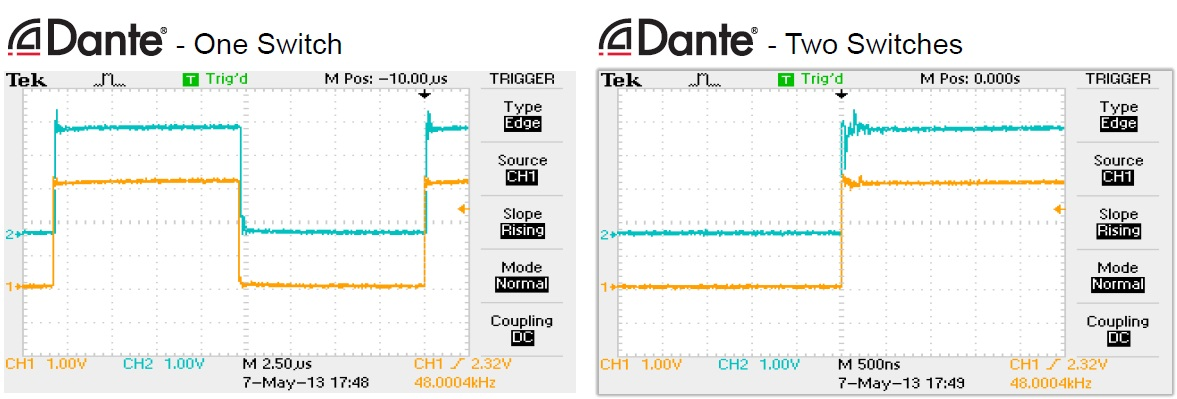
\includegraphics[width=400px, keepaspectratio] {figures/dante-clocking.jpg}
	\caption{Dante órajel}
	\label{fig:dante-clock}
\end{figure}
%----------------------------------------------------------------------------

%----------------------------------------------------------------------------
\subsection{Összehasonlítás a hagyományos hangrendszerekkel}
%----------------------------------------------------------------------------
A hagyományos hangrendszerek általában analóg kábelekre és csatlakozókra
támaszkodnak a hangjelek eszközök közötti átviteléhez. Ezek a rendszerek
korlátozottak lehetnek rugalmasságban, skálázhatóságban és az egyidejűleg
átvihető hangcsatornák számában. Emellett hajlamosak bonyolultabbá válni a
beállítás és kezelés szempontjából, mivel minden hangcsatornához külön kábel és
csatlakozás szükséges. A Dante hanghálózatok jóval több hangcsatornát is támogatnak,
mint a hagyományos analóg rendszerek, és távolról is vezérelhetők és
monitorozhatók, lehetővé téve a nagy, összetett hangrendszerek könnyű
beállítását és kezelését. A Dante hanghálózatok további előnye, hogy képesek
hangot továbbítani hosszú távolságokon anélkül, hogy a minőség romlana. A
hagyományos analóg rendszerek zajra és jelveszteségre hajlamosak hosszú kábelek
esetén, míg a digitális hangjelek, amelyeket az Ethernet hálózatokon
továbbítanak, minimális minőségveszteséggel juthatnak el nagy távolságokra.
%----------------------------------------------------------------------------
\begin{table}[htbp]
    \centering
    \caption{Digital Snake és DigitalAVNetwork Jelút opciók}
    \begin{tabular}{@{}lll@{}}
        \toprule
        \textbf{Kérdés} & \textbf{Pont-pont között} & \textbf{Hálózati megoldás} \\ \midrule
        Hová megy a jel? & Lineáris kábelút & Bárhol a hálózaton \\
        Hogyan változtassuk meg a jelútvonalat? & Mozgassuk a kábelt & Egy egérkattintással \\
        Szétválaszthatjuk-e a jeleket? & Nem & Igen - a hálózaton \\
        Megosztható-e a kábel más jelekkel? & Nem & Igen - közös infrastruktúra \\
        \bottomrule
    \end{tabular}
    \label{tab:digital-snake-vs-digitalavnetwork-hu}
\end{table}
%----------------------------------------------------------------------------
\begin{figure}[H]
	\centering
	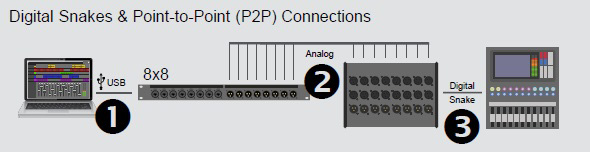
\includegraphics[width=\linewidth, keepaspectratio]{figures/dsnake-p2p.jpg}
	\caption{Digital Snake és Pont-pont közötti (P2P) kapcsolatok}
	\label {fig:dsnake-p2p}
\end{figure}
%----------------------------------------------------------------------------
\begin{figure}[H]
	\centering
	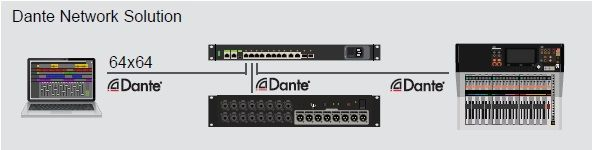
\includegraphics[width=\linewidth, keepaspectratio]{figures/dante-solution.jpg}
	\caption{Dante hálózati megoldás}
	\label {fig:dante-solution}
\end{figure}
%----------------------------------------------------------------------------

A rugalmasság és a skálázhatóság tovbbi kulcsfontosságú előnye a Dante
hanghálózatoknak a hagyományos analóg hangrendszerekkel szemben.
Képesek alkalmazkodni különböző hangkonfigurációkhoz és követelményekhez. 
Könnyű eszközöket hozzáadni vagy eltávolítani, megváltoztatni a hangjelek útvonalát, és a rendszert újra
konfigurálni szükség esetén. Ez lehetővé teszi testreszabott audio-megoldások
létrehozását, amelyeket az adott alkalmazás vagy környezet speciális igényeihez
lehet igazítani. 

%----------------------------------------------------------------------------
\subsection{Firmware frissítés}
%----------------------------------------------------------------------------

A Dante eszközök rendelkeznek Dante Firmware és Eszköz Firmware-el.
Lehet, hogy mindkettőt frissíteni kell. Kérjük, forduljon a gyártóhoz a párosított verziókért.
Néhány eszköz sorozat más módszerekkel frissíthető.
A Dante Updater hasznos lehet a frissítések nyomon követéséhez és telepítéséhez.
A rendszer ellenőrzi az online adatbázisunkat, hogy tájékoztassa Önt az elérhető frissítésekről.
A Dante firmware könnyen frissíthető.
A Dante Firmware Update Manager továbbra is aktuális.
Importálja a firmware fájlokat, ha firmware-t kap egy gyártótól.
Ha a frissítés nem sikerül, rendelkezünk vészhelyzeti helyreállítási módszerrel.
A Dante eszközök erős támogatást nyújtanak a vegyes firmware verziókhoz.
Mérnökeink automatizált regressziós tesztelést végeztek a korábbi firmware kiadásokkal szemben.

%----------------------------------------------------------------------------
\subsection{Chipek}
%----------------------------------------------------------------------------

A Dante hálózatok változatos chipekkel építhetők fel. 
Az Audinate számos különböző chipet kínál a Dante hálózatok létrehozásához, 
melyek eltérő hangcsatorna-számot és egyéb funkciókat támogatnak. 
A Dante chipek különféle méretekben és árkategóriákban elérhetők, 
lehetővé téve a gyártók számára, hogy különféle méretű és árú Dante 
eszközöket fejlesszenek ki, így képesek kielégíteni a különböző piaci igényeket. 
A Dante chipek segítik a gyártókat abban, hogy gyorsan és hatékonyan hozzanak 
létre Dante-kompatibilis eszközöket, és könnyedén integrálják azokat a saját termékeikbe.

%----------------------------------------------------------------------------
\begin{center}
	\begin{tabular}{|c|p{10cm}|}
		\hline
		\textbf{Chip} & \textbf{Leírás} \\
		\hline
		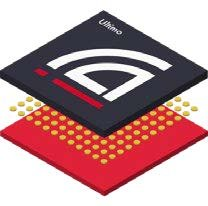
\includegraphics[width=40px,height=40px,keepaspectratio]{figures/ultimo-x.jpg} & \textbf{Dante Ultimo-X} - 0x4, 2x2, 4x0 \\
		\hline
		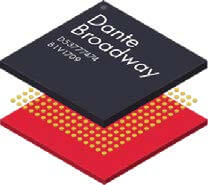
\includegraphics[width=40px,height=40px,keepaspectratio]{figures/broadway.jpg} & \textbf{Dante Broadway} - 16x16 \\
		\hline
		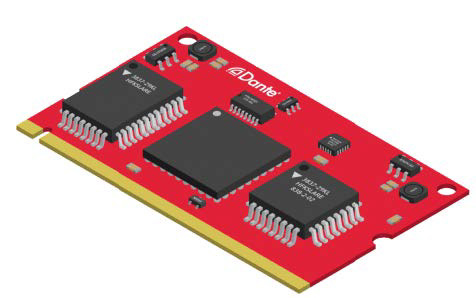
\includegraphics[width=40px,height=40px,keepaspectratio]{figures/brooklyn-ii.jpg} & \textbf{Dante Brooklyn II} - 64x64 \\
		\hline
		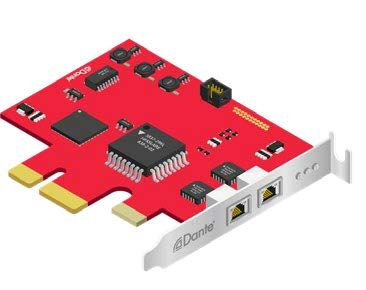
\includegraphics[width=40px,height=40px,keepaspectratio]{figures/pcie-r.jpg} & \textbf{Dante PCIe-R} - 128x128 \\
		\hline
		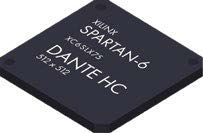
\includegraphics[width=40px,height=40px,keepaspectratio]{figures/dante-hc.jpg} & \textbf{Dante HC (High Capacity)} - 512x512 \\
		\hline
		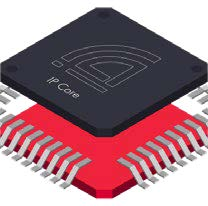
\includegraphics[width=40px,height=40px,keepaspectratio]{figures/shared-processor.jpg} & \textbf{Dante Shared Processor} - IP Core 512x512 FPGA and Dante Embedded Platform 64x64 X86/ARM \\
		\hline
		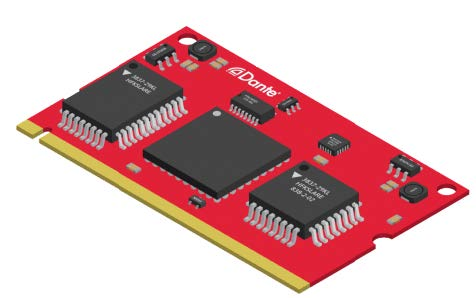
\includegraphics[width=40px,height=40px,keepaspectratio]{figures/dante-av.jpg} & \textbf{Dante AV} - V:1, A:8 \\
		\hline
	\end{tabular}
\end{center}
%----------------------------------------------------------------------------
	







%----------------------------------------------------------------------------
\chapter{\SystemDesign}
%----------------------------------------------------------------------------
\section{Követelmények}
%----------------------------------------------------------------------------
Az új rendszer tervezésekor a következő szempontokat kellett szem előtt tartanom:
\begin{itemize}
	\item Teljesen digitális megoldás kialakítása.
	\item Redundáns rendszer kialakítása biztosítva a folyamatos működést.
	\item Rugalmas felépítés, amely lehetővé teszi a könnyű alkalmazkodást változó körülményekhez.
	\item Könnyen bővíthető struktúra kialakítása a jövőbeli igényekhez való gyors reagálás érdekében.
	\item Magasabb hangminőség és hangnyomás elérésének lehetősége a korábbi rendszerrel összehasonlítva.
	\item Jobb lefedettség és egyenletes hangvisszaadás biztosítása a közönség területén.
	\item A piacon lévő termékekhez képest viszonylag költséghatékony megoldás kidolgozása.
	\item Legyen hosszú távon egy kompetitív és korszerű rendszer.
	\item Megbízható és kiforrott technológiára épüljön.
\end{itemize}
%----------------------------------------------------------------------------
\section{Rendszerterv}
%----------------------------------------------------------------------------
A szakdolgozatomban megtervezésre kerülő hangrendszer lelke a Dante protokoll lesz.
Hangládák szempontjából a Martin Audio Wavefront Precision szériás termékeire esett a választás.
Mivel teljes mértékben digitális rendszert elérése volt a cél, ezért a Dante modullal
rendelkező Martin Audio iKON iK42 és iK81 végfokok tökéletesen illeszkedtek a rendszerbe.
Mindkét végfok csúcskategóriás teljesítményt és hangminőséget nyújt, és a D kategóriás
erősítőknek köszönhetően rendkívül kis helyet foglalnak el a rack-ben miközben kiváló hatásfok
mellett képesek nagy teljesítményt leadni. A két erősítő között két fundamentális különbség van,
az iK42 négy kimeneti csatornával rendelkezik, 20.000 W teljesítmény leadása mellett. 
Ezzel szemben az iK81 nyolc kimeneti csatornával rendelkezik, 10.000 W teljesítménnyel. \cite{IKONAMPUSEGUIDE}
A végfokokat a Dante hálózaton keresztül fogjuk jellel ellátni, így a hagyományos analóg XLR, vagy AES kábelezés helyett
két CAT5E kábellel (a redundancia miatt) tudjuk a végfokokat a hálózatra kötni. 
%----------------------------------------------------------------------------
\begin{figure}[H]
    \centering
    \begin{minipage}{0.45\textwidth}
        \centering
        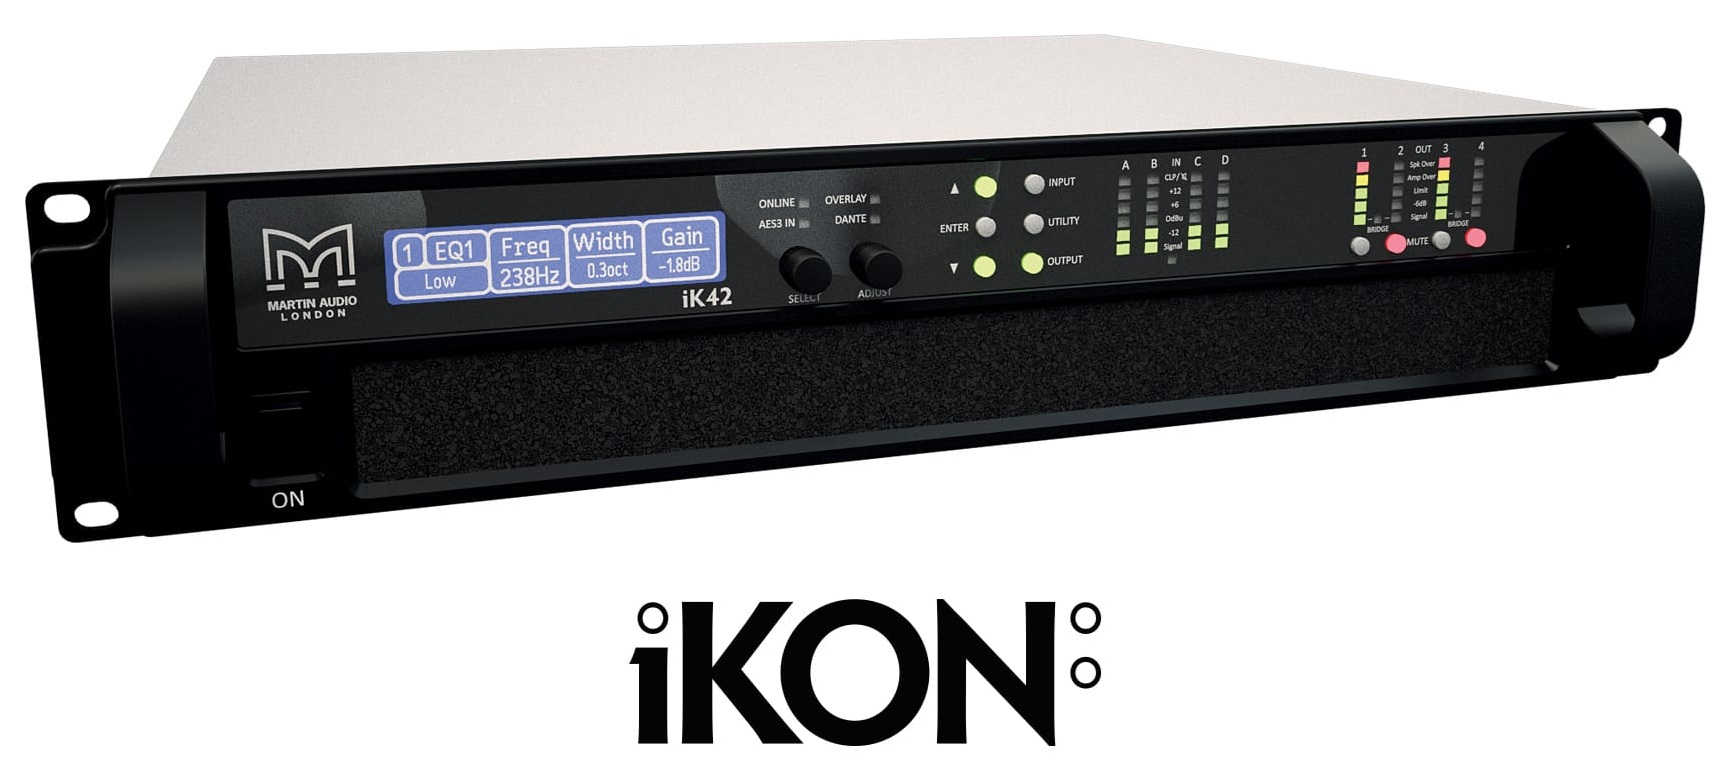
\includegraphics[width=\linewidth, keepaspectratio]{figures/ikon_ik42.jpg}
        \caption{Martin Audio iK42 végfok}\label{fig:ikon_ik42}
    \end{minipage}\hfill
    \begin{minipage}{0.45\textwidth}
        \centering
        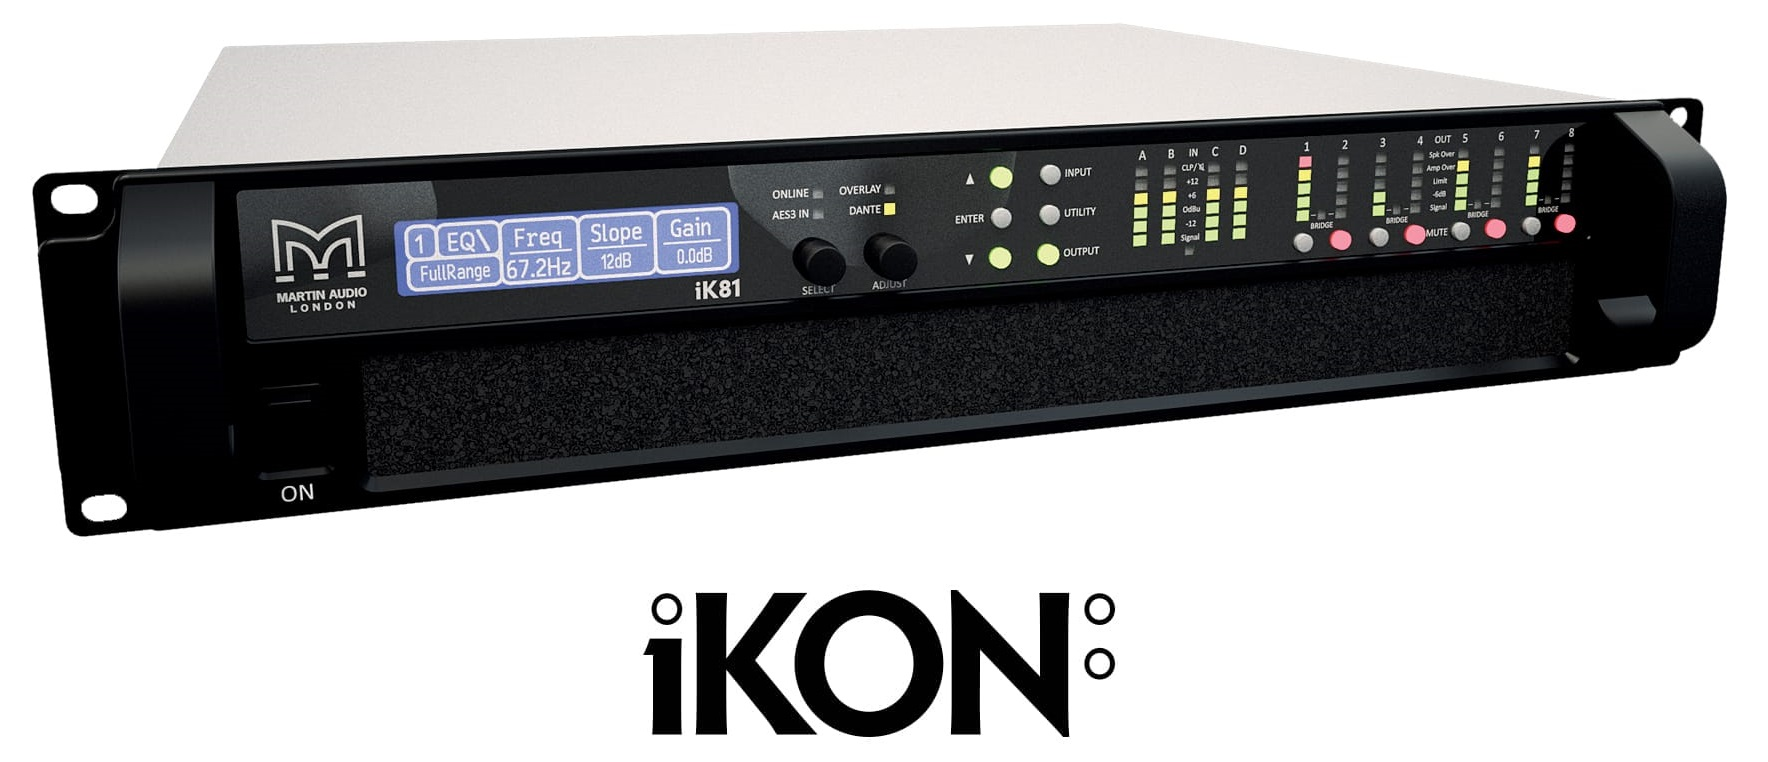
\includegraphics[width=\linewidth, keepaspectratio]{figures/ikon_ik81.jpg}
        \caption{Martin Audio iK81 végfok}\label{fig:ikon_ik81}
    \end{minipage}
\end{figure}
%----------------------------------------------------------------------------
A végfokrendszer fő vezérlő protokollja miatt szükség lesz még egy CAT5E alapú
összeköttetésre, ami az egyes végfokokat köti össze egy hálózatba a switcheken keresztül. (VU-NET protokoll)
Minden egyes végfokrackben két MikroTik 24 portos switch lesz. Az egyik switch a Dante elsődleges hálózatát fogja kizárólag kezelni.
A másik switch a Dante másodlagos hálózatát, és a VU-NET hálózatot fogja kezelni.
Ez a két alhálózat VLAN szegmensekkel lesz elkülönítve, hogy a hálózat biztonságos és stabil legyen.
A rendszer kábelezése egyedileg készített Neutrik EtherCon csatlakozóval ellátott CAT5E és CAT6A kábelekből fog állni.
A kábelek készítésekor a T568B szabvány szerinti kábelrendezést alkalmazom, mivel a T568B jobb átviteli
teljesítményt és interferencia védelmet nyújt a hosszú távú használat során.
Nem szükséges a T568A szabvány által nyújtott plusz kompatibilitás a régi hálózatokkal, mivel egy teljesen új 
modern hálózatot fogunk kiépíteni. 
A csatlakozók felhelyezésekor a szabványnak megfelelően járok el, milliméterre pontosan, hogy a kábelek
a lehető legjobb minőségűek legyenek. Ez a CAT6A kábeleknél különösen fontos, mivel a CAT6A kábelek
még nagyobb frekvencia tartományban képesek adatokat továbbítani, mint a CAT5E kábelek,
ezért jobban érzékenyek a külső interferenciákra.

%----------------------------------------------------------------------------
\begin{figure}[H]
	\centering
	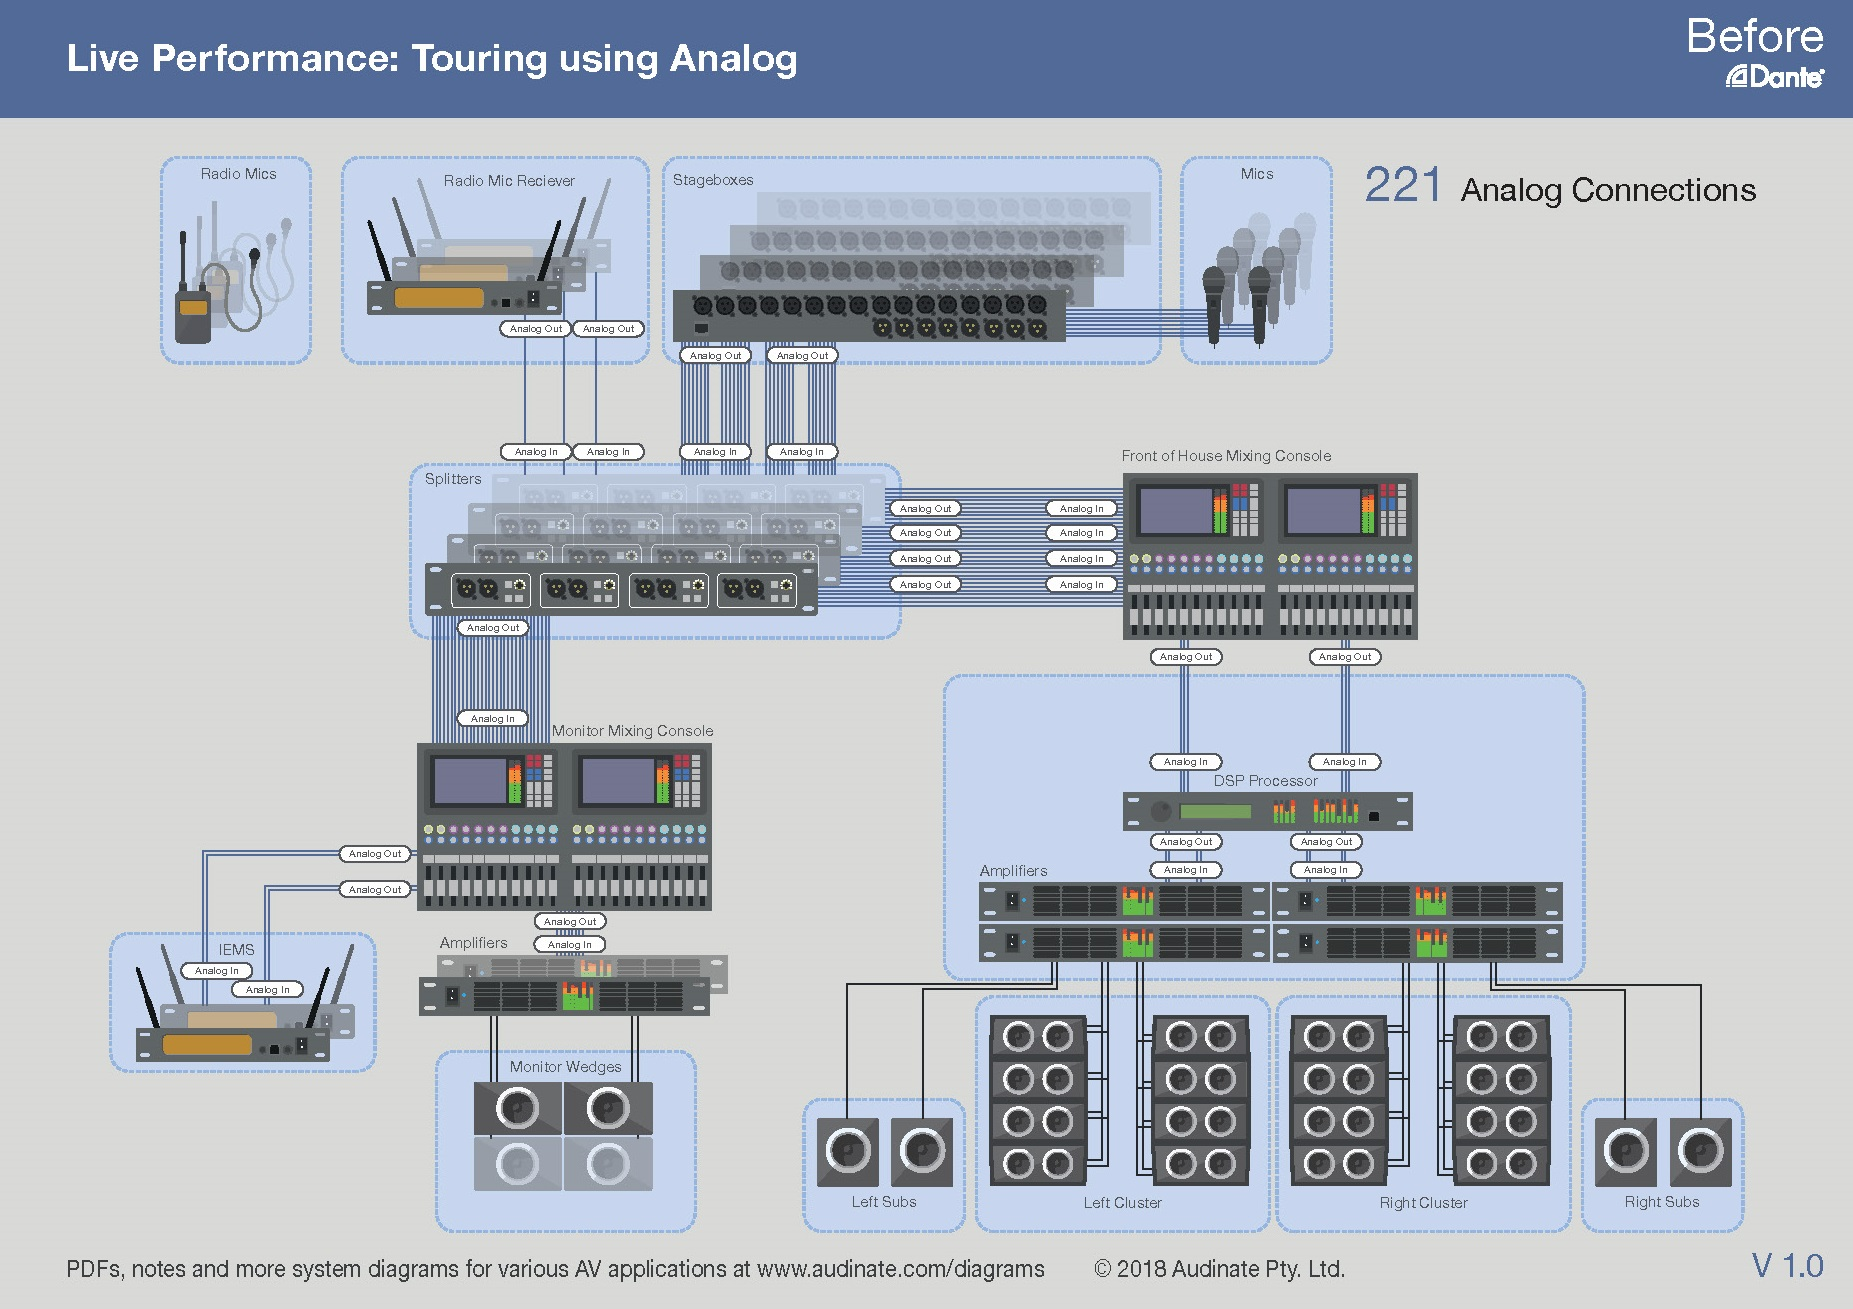
\includegraphics[width=\linewidth, keepaspectratio]{figures/live-analog.jpg}
	\caption{Hagyományos analóg kábelezés \cite{APPLICATIONDIAGRAMSFORDANTESYSTEMS}}\label{fig:live-analog}
\end{figure}
%----------------------------------------------------------------------------
\begin{figure}[H]
	\centering
	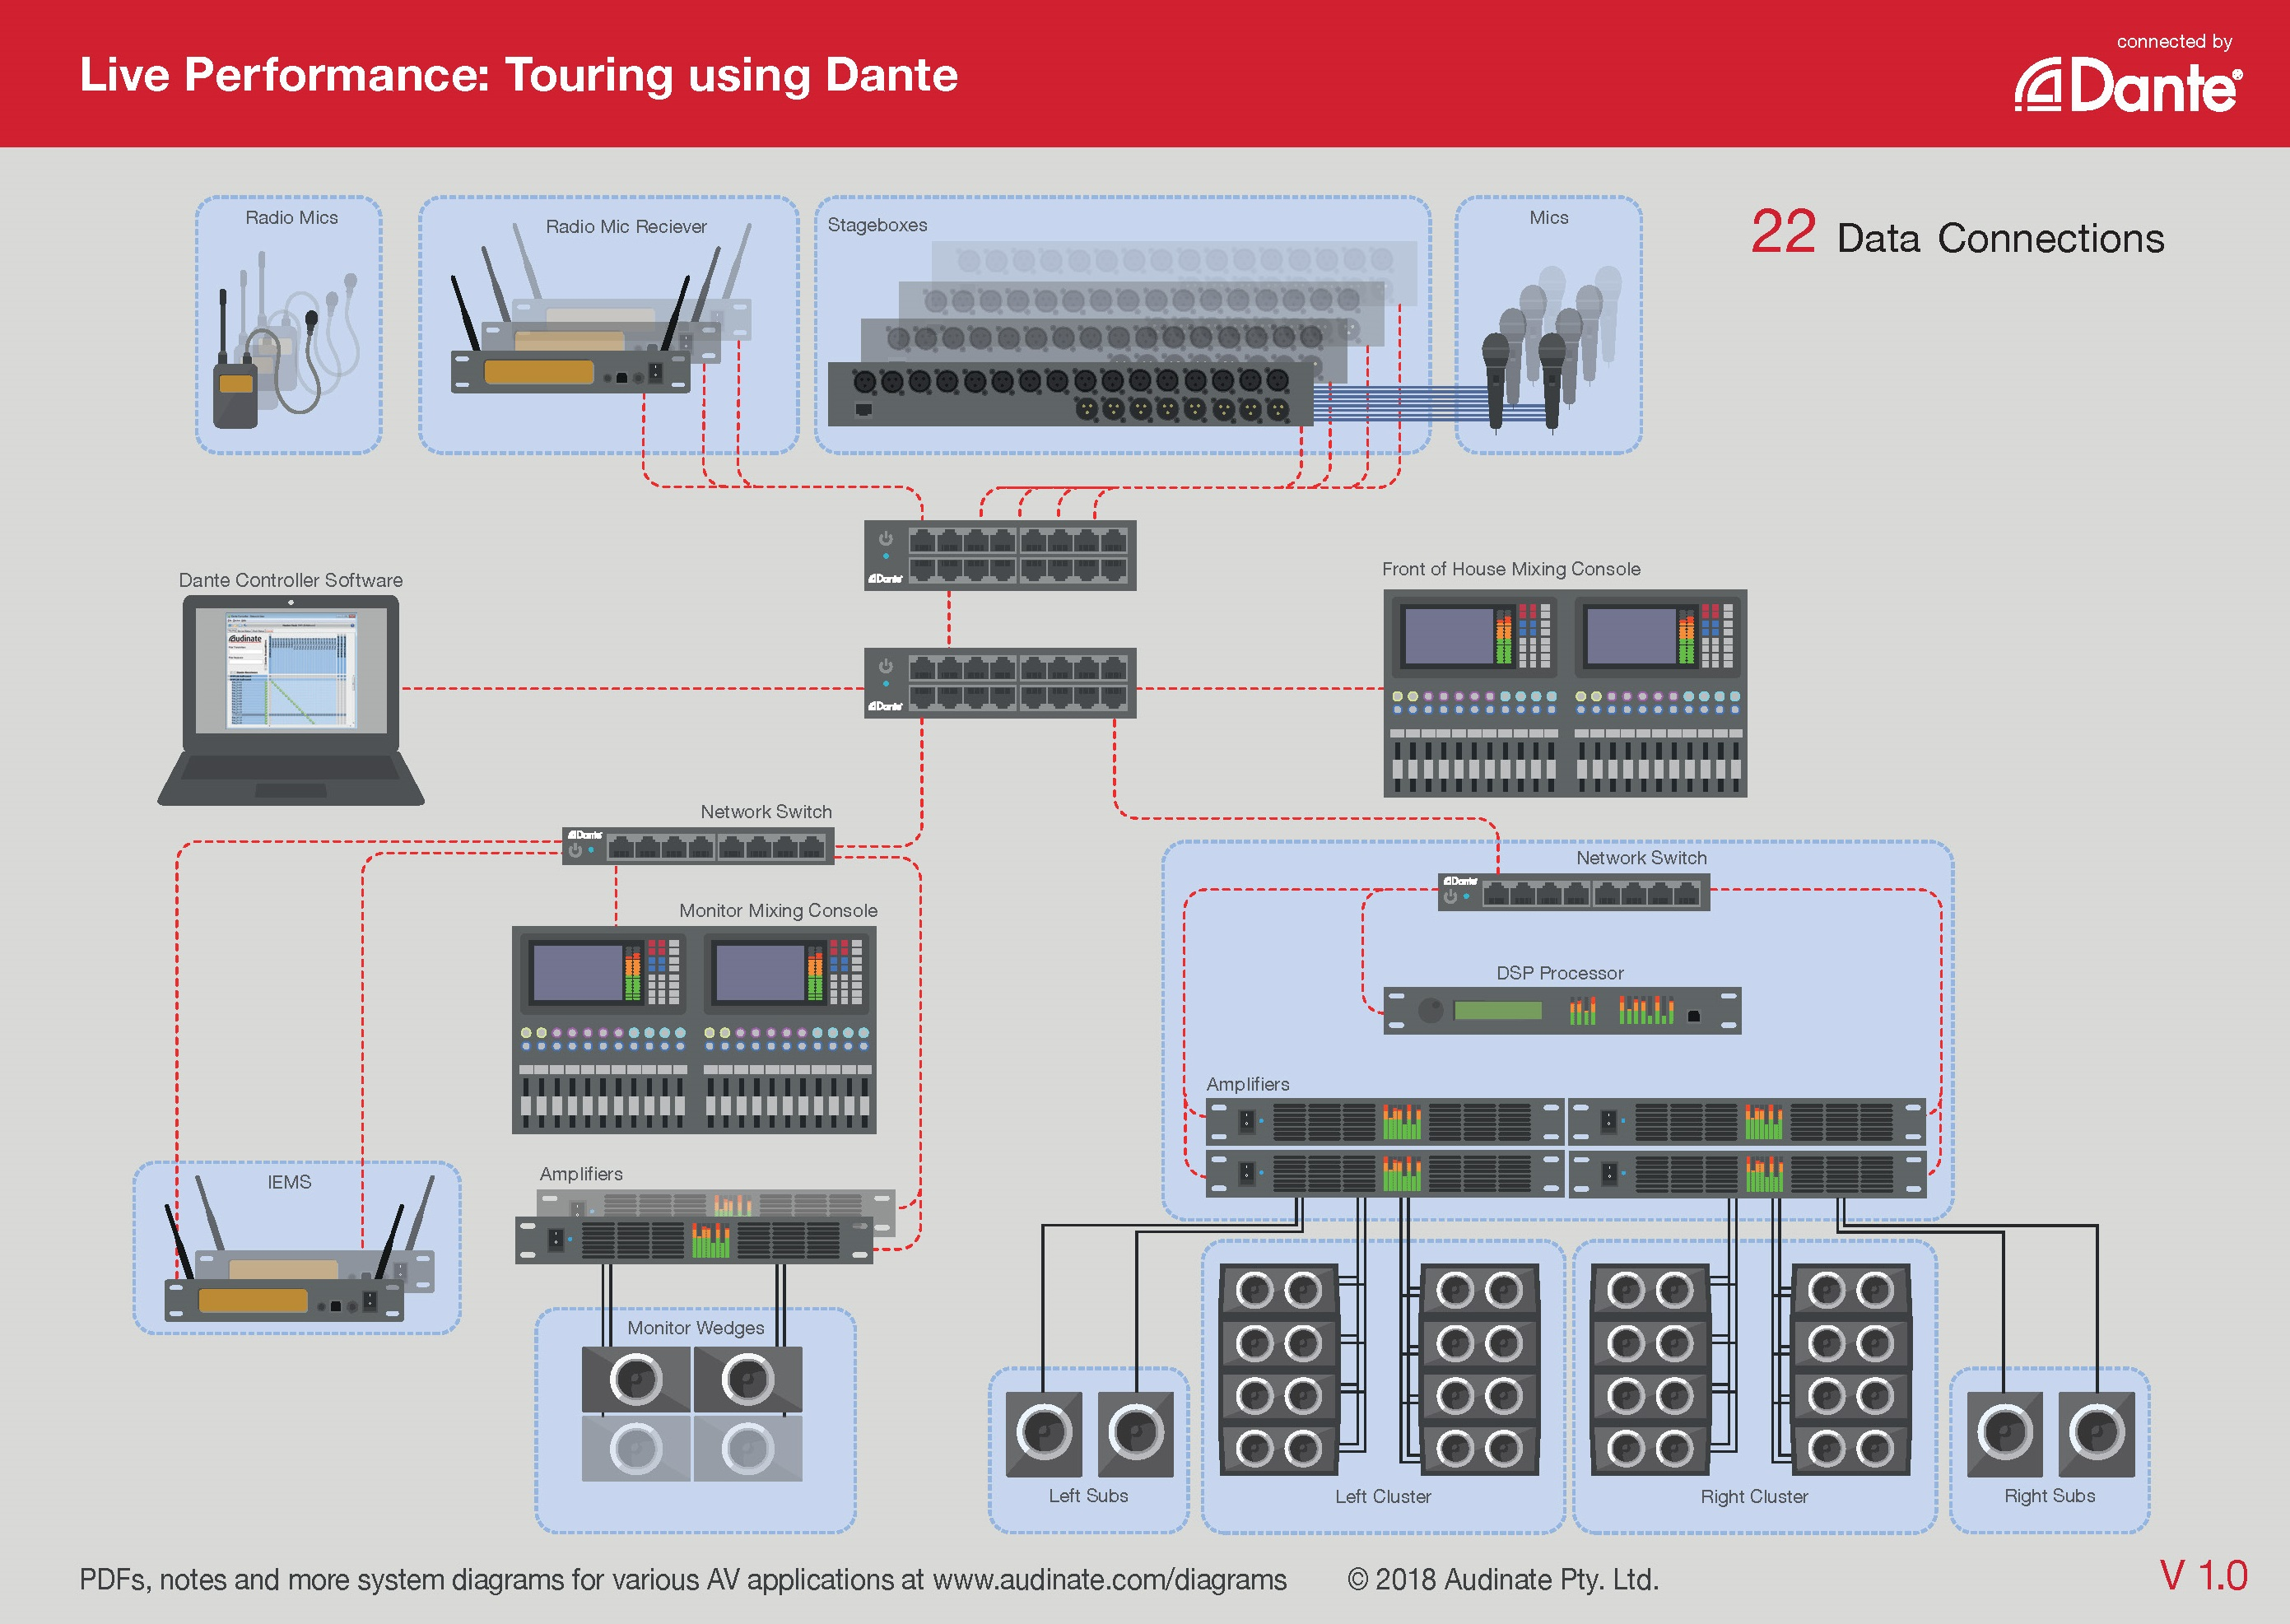
\includegraphics[width=\linewidth, keepaspectratio]{figures/live-dante.jpg}
	\caption{Dante digitális kábelezés \cite{APPLICATIONDIAGRAMSFORDANTESYSTEMS}}\label{fig:live-dante}
\end{figure}
%----------------------------------------------------------------------------

%----------------------------------------------------------------------------
\subsection{Martin Audio Wavefront Precision hangrendszer}
%----------------------------------------------------------------------------
\subsubsection{Martin Audio Display 2.3.4 b1 tervező szoftver \cite{DISPLAY23USERGUIDE}}
%----------------------------------------------------------------------------
Mielőtt bele fognánk a tervezési folyamatba, fontos megemlíteni, hogy a szoftver
eredetileg Intel alapú processzorokra lett tervezve és MatLab alapú. Ebből fakadóan
AMD Ryzen processzorokon habár elindult a szoftver, de nem volt stabil és a számítások során
minden esetben összeomlott, és használhatatlanul lassú volt. Személy szerint a saját gépem amivel dolgoztam
sajnos ilyen processzorral van szerelve ezért muszáj volt megoldást találni a problémára.
A Martin Audio hivatalos szoftveres támogatásához fordultam először, de sajnos nem tudtak segíteni.
Ezért a szoftver használatához
sok belefektetett óra olvasás után sikerült egy olyan MatLab CMD parancsot találnom, amivel
a szoftver elindul és használható.
Miután rájöttem a probléma gyökerére, ezt megosztottam velük, hogy a jövőben másoknak ne kelljen
ezzel a problémával szembesülniük.
A hiba az alábbi volt. Az új AMD Ryzen processzorok másfajta utasításkészletet használnak.
Ebből kifolyólag a MatLab 2015-s runtime alapú szoftver adta alaputasításokat nem tudta értelmezni a CPU.
A vezető szoftvermérnökkel való e-mail-es beszélgetésünk során megköszönte a probléma
megoldását, és nemsokkal a megoldásom megosztása után a hivatalos oldalra is felekerült
az indító parancsfájl. Az e-mailben további kollaborációra is adott lehetőséget.
A kompatibilitási problémát rögtön a script elején megoldottam,
mivel a következő parancs megadásával már használhatóvá válik a program: \texttt{set MKL\_DEBUG\_CPU\_TYPE=5} \newline
Ez a sor a program vezérlését AVX2-re állítja át, és mivel ezt az utasításkészletet már ismeri az AMD Ryzen processzor
is ezért a probléma már a múlté.
Az indító fájl további sorai optimalizálások a számítások gyorsítására, és a párhuzamosítására, ezzel jobban kihasználva
a rendelkezésre álló hardver erőforrásokat.
%----------------------------------------------------------------------------
\begin{lstlisting}[caption={A Display 2.3.4 b1 indító ".bat" scriptje AMD Ryzen processzorokhoz}, label=batcode, xleftmargin=\parindent]
    @echo off
    set PATH=%PATH%;C:\Program Files\Martin Audio\Display2_3_4_b1\application
    set MKL_DEBUG_CPU_TYPE=5
    set options=optimoptions('ga','UseParallel',true,'UseVectorized',false)
    set options=optimoptions('gamultiobj','UseParallel',true,'UseVectorized',false)
    set options=optimoptions('paretosearch','UseParallel',true)
    set options=optimoptions('particleswarm','UseParallel',true,'UseVectorized',false)
    set options=optimoptions('patternsearch','UseParallel',true,'UseCompletePoll',true,'UseVectorized',false)
    set options=optimoptions('surrogateopt','UseParallel',true)
    set GPUAcceleration=on
    start "Martin Audio" Display2_3_4_b1.exe
    pause
\end{lstlisting}
%----------------------------------------------------------------------------
\begin{figure}[H]
	\centering
	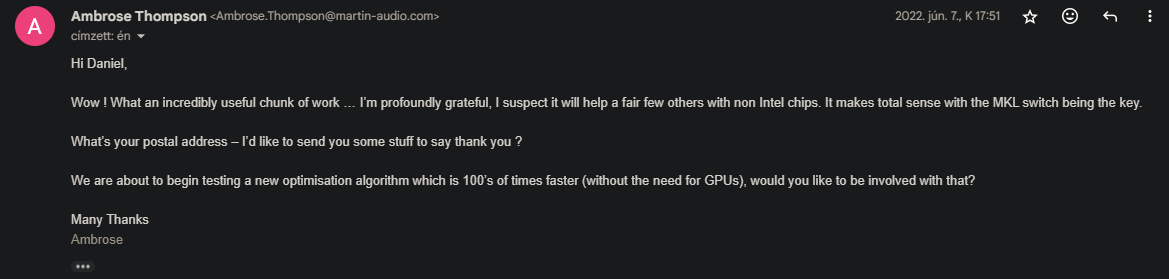
\includegraphics[width=\textwidth, keepaspectratio]{figures/ambrose_email.png}
	\caption{E-mail a Martin Audio vezető szoftvermérnökétől}
	\label{fig:ambrose_email}
\end{figure}
%----------------------------------------------------------------------------
Most, hogy már a szoftver használható és teljes mértékben működőképes, kezdjük el a tervezést.
A modellezés során a budapesti Millenáris B csarnoka lesz a referencia helyszín. Két LineArray rendszert fogunk
tervezni, mivel a terem hosszúsága és a lefedettség növelése miatt szükségünk lesz Delay kiegészítésre a fő hangrendszerhez.
Első lépésben a fő hangrendszert tervezem meg, ami oldalanként (bal és jobb) 8 darab WPC LineArray modulból fog állni.
Ez a láda 2 darab 10"-os mélysugárzót (LF), 2 darab 5"-os közép sugárzót (MF) és 4 darab 0.7"-os magassugárzót tartalmaz (HF).
Három utas Bi-amp meghajtású külső végfokot igénylő rendszer, ahol a mély tartományt (+1,-1) és a középmagas tartományt (+2,-2) külön kezeljük,
a négy pólusú Neutrik Speakon csatlakozókon keresztül.
A láda maximális hangnyomás szintje 135 dB, és 65 Hz-től 18 kHz-ig terjed a frekvencia átvitele +- 3 dB pontossággal. \cite{WPCUSERGUIDE}
%----------------------------------------------------------------------------
\begin{figure}[H]
	\centering
	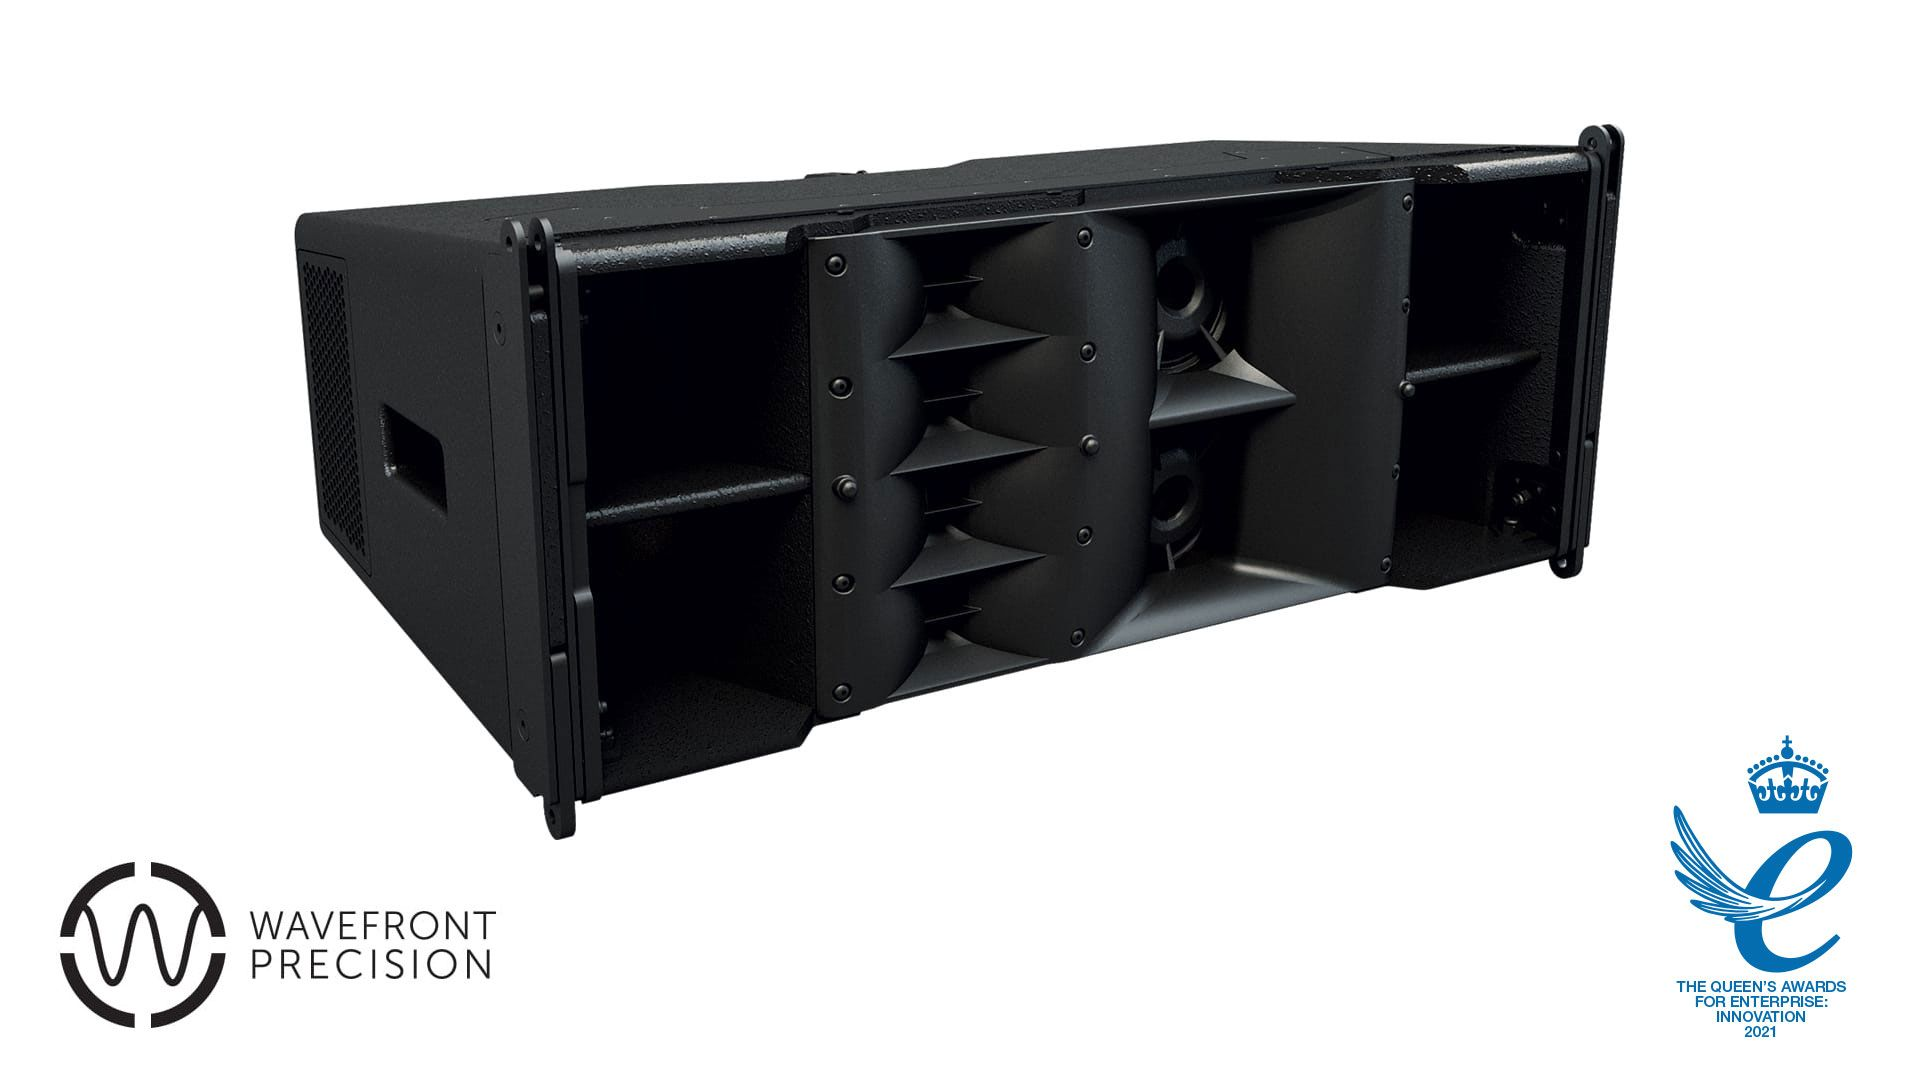
\includegraphics[width=80mm, keepaspectratio]{figures/wpc_front_view.jpg}
	\caption{Martin Audio WPC LineArray modul}\label{fig:wpc}
\end{figure}
%----------------------------------------------------------------------------
A program megnyitásakor a legelső lépés, hogy kiválasztjuk a termékpalettából a megfelelő hangrendszert.
Jelen esetben az előbbiekben említett WPC-t. A produkció igényei, a nagy létszámú közönség és a ládamennyiség miatt a rendszert
\textit{``riggelni''} fogjuk. (maximálisan 6 darab WPC-t lehet \textit{``stackelni''}, azaz a földre vagy mélyládákra helyezni)
A helyszín felmérése után a hangrendszer \textit{``riggelése''} lehetséges, mivel a csarnokban található tartószerkezet biztonságosan
és tartósan képes elviselni a rendszer súlyát.
A telepítés módja kiválasztása után megadjuk a szoftvernek a tervezni való hangláda mennyiséget, ez az esetünkben már említett 8 darab.
A hozzáadás gombra kattintva a elénk kerül a fő kezelőfelület, ahol a hangrendszert tudjuk lépésről lépésre tervezni.
%----------------------------------------------------------------------------
\begin{figure}[H]
	\centering
	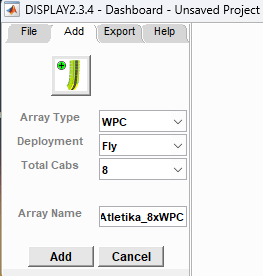
\includegraphics[width=40mm, keepaspectratio]{figures/display_wpc_0.png}
	\caption{Display 2.3.4 b1 kezdőképernyője (WPC)}\label{fig:display_wpc_0}
\end{figure}
%----------------------------------------------------------------------------
A tervezési folyamat öt részre osztható, amiket a szoftverben külön kezelünk.
Ezeket a \textit{``Slice''}, \textit{``Cover''}, \textit{``Splay''}, \textit{``Rig''} és \textit{``EQ''} kezelőfelületeken tudjuk elvégezni,
balról jobbra haladva. Mivel a különböző részegységek egymásra épülnek, ezért fontos a sorrend betartása.
(tervezés utáni módosításokra természetesen van lehetőség, de az adott projekt első tervezési folyamata során ezeket a lépéseket kell követni)
%----------------------------------------------------------------------------
\begin{figure}[H]
	\centering
	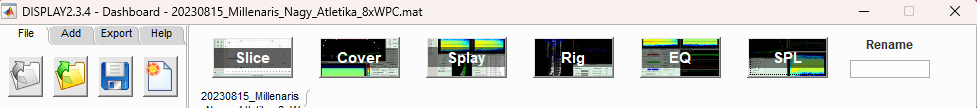
\includegraphics[width=\textwidth, keepaspectratio]{figures/display_wpc_0_1.png}
	\caption{Display 2.3.4 b1 fő kezelőfelülete (WPC)}\label{fig:display_wpc_0_1}
\end{figure}
%----------------------------------------------------------------------------
A \textit{``Slice''} panelen meghatározzuk a rendszer fizikai pozícióját térben. A csarnok
pontos lemodellezése érdekében a mérésekhez lézeres távolságmérőt használtam.
Mivel minden egyes rendezvényen más és más a különböző elemek elhelyezkedése, ezért a
rendszert minden alkalommal újra kell tervezni, még akkor is ha maga a helyszín nem változik.
\textit{``Vertex''} pontok segítségével tudjuk a méreteket és a pozíciókat meghatározni.
A 2D-s modellen figyelembe kell venni a terem önálló méretén kívül a színpadod és a színpad mögötti területet is.
A rajznak tartalmazni kell azokat a falfelületeket is amelyeknél a hangvisszaverődést minimalizálni szeretnénk,
ennek az optimalizáció későbbi fázisában lesz jelentősége.
A terem pontos rajza után még két fontos paramétert kell megadni ezen a felületen.
El kell helyeznünk magát a hangrendszert a teremben, és meg kell határoznunk milyen magasra szeretnénk a rendszert emelni.
Mivel a csarnok rendkívül hosszú, és a adottságai megengedik, ezért a rendszert minél magasabbra szeretnénk emelni,
a jobb lefedettség érdekében.
A másik fontos paraméter az optimalizációhoz, a közönség területének meghatározása. Kezdő és végpont segítségével
tudjuk a területet meghatározni, ahol a hallgatóközönség tartózkodni fog.
%----------------------------------------------------------------------------
\begin{figure}[H]
	\centering
	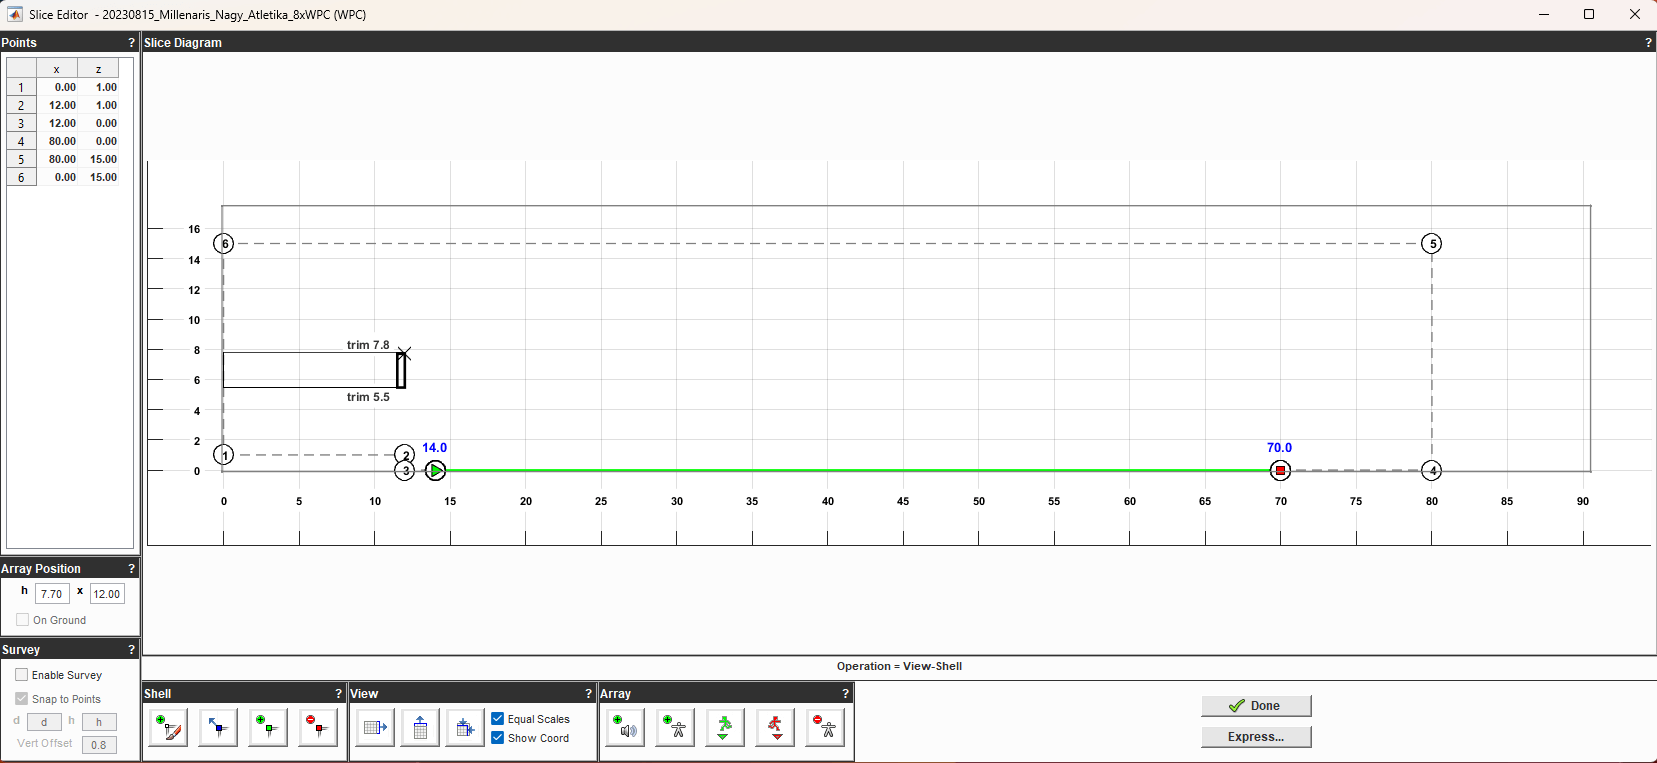
\includegraphics[width=\textwidth, keepaspectratio]{figures/display_wpc_1.png}
	\caption{Display 2.3.4 b1 \textit{``Slice''} kezelőfelülete (WPC)}\label{fig:display_wpc_1}
\end{figure}
%----------------------------------------------------------------------------
A következő lépések a \textit{``Cover''} kezelőfelületen történnek.
Első és legfontosabb beállítás amit el kell végezni, hogy a hallgatóság az esemény során ülni vagy állni fog-e.
Lehetőségünk van a nézőteret különböző részekre is osztani, amennyiben a rendezvény során különböző helyeken
eltérő típusú részeket szeretnénk egyenletesen lefedni. Lehetőség van egyedi magasság beállítására is,
de jelen esetben a közönség egyhangúan állva fogja hallgatni a produkciót, ezért a \textit{``Standing''} opciót választottam.
Az előző lépésben elkészített rajzunkon definiálhatunk a program számára három fő régiót.
\newline Ezek az alábbiak:
%----------------------------------------------------------------------------
\begin{itemize}
	\item \textit{``Non Audience''} - a közönség területén kívül eső terület
	\item \textit{``Audience''} - a közönség területe
	\item \textit{``Hard Avoid''} - a közönség területén kívül eső terület, ahol a hangvisszaverődést szeretnénk minimalizálni
\end{itemize}
%----------------------------------------------------------------------------
Jelen esetben a fő hangrendszernél nem jelöltem meg a \textit{``Hard Avoid''} területet, mivel a teremben az első olyan felület
ami a hangvisszaverődést okozna már olyan távol helyezkedik el a hangrendszertől, hogy a hangvisszaverődés már nem okoz problémát.
A következő lépéseket előkészítve meg kell határoznunk a hangrendszertől egy adott távolságra lévő pontot a teremben,
amit referencia pontként fogunk használni. Ezt a pontot a \textit{``Move Ref''} gombra kattintva tudjuk megadni,
vagy manuálisan beírva az X és Y koordinátákat. Automatikusan a terem közepére van pozícionálva a referencia pont, de
ezt erősen ajánlott mozgatni attól függően mit szeretnénk elérni. Jelen esetben a mix pultot fogjuk a referencia pontnak megadni.
A \textit{``Start''} és \textit{``Stop''} mezőkben meg kell adnunk, hogy a referencia ponttól véve mekkora hangnyomás
deltával szeretnénk dolgozni. Ez azt jelenti, hogy a kezdő, a referencia és a végpont közötti hangnyomás hány dB-el térhet el egymástól.
Ezt az értéket a szoftver az eddig megadott információk alapján automatikusan kiszámolja, de manuálisan is megadhatjuk.
Az automatikus számítás az esetek többségében megfelelő eredményt ad, ezért most is ezt választottam.
A \textit{``Target SPL''} mezőben megadhatjuk a referencia ponton elérni kívánt hangnyomás szintet.
Így a rendszer \textit{``Gain''} struktúrája úgy lesz beállítva, hogy a referencia ponton 0 dBu bemeneti szint mellett elérjük a megadott hangnyomás szintet.
Magas frekvenciák csökkennek ahogy a távolság nő a forrástól, azaz a hangrendszertől.
Ha egyenletes frekvencia választást szeretnénk elérni nagyobb távolságokon, akkor a rendszernek nagyobb energiára lenne szüksége
a magas frekvenciákon, és kifutna a dinamika tartalékból, ezért jobb megoldás, ha a magas frekvenciák fokozatosan csökkennek a távolság növekedésével.
Beállíthatjuk a levegő veszteség kompenzációját, teljesen balra állítva nincs kompenzáció (figyelmen kívül hagyva a levegő abszorpcióját).
Teljesen jobbra állítva a maximális kompenzáció (a rendszernek 17dB headroom-ra van szüksége, hogy egyenes választ kapjunk).
Viszont ezekből az következik, hogyha túlságosan sok a kompenzáció, akkor a rendszernek nem lesz elég dinamika tartaléka, és a hang torzulni fog.
A változások hatását a \textit{``Target Response''} ábrán láthatjuk.
Ahhoz, hogy a számítások pontosak legyenek, elengedhetetlen, hogy pontosan megadjuk a környezeti változókat,
a hőmérsékletet, a páratartalmat és a légnyomást. Ezeket a paramétereket a \textit{``Edit''} gombra kattintva tudjuk megadni.
Jelen esetben mivel a teremben alapból is meleg van, a mérés időpontjában 28 fok, és a rendezvény során a közönség is melegíti a termet,
ezért a hőmérsékletet harminc fokra állítottam.
A páratartalom értéke a méréskor 57\%-os volt, de én 65\%-ra állítottam, mivel a rendezvény során a közönség által kibocsátott
vízgőz miatt a páratartalom nagy valószínűséggel magasabb lesz ennél. A légnyomás értékét pedig a helyi időjárás jelentésből vettem, ami
azon a napon 101800 Pa volt. Ezek beállítása után mivel az adott hangládához a gyári beállítások nagyon jók, ezért nem változtattam rajtuk,
a 14-es érték egyenletes és dinamikus hangvisszaadást biztosít.
%----------------------------------------------------------------------------
\begin{figure}[H]
	\centering
	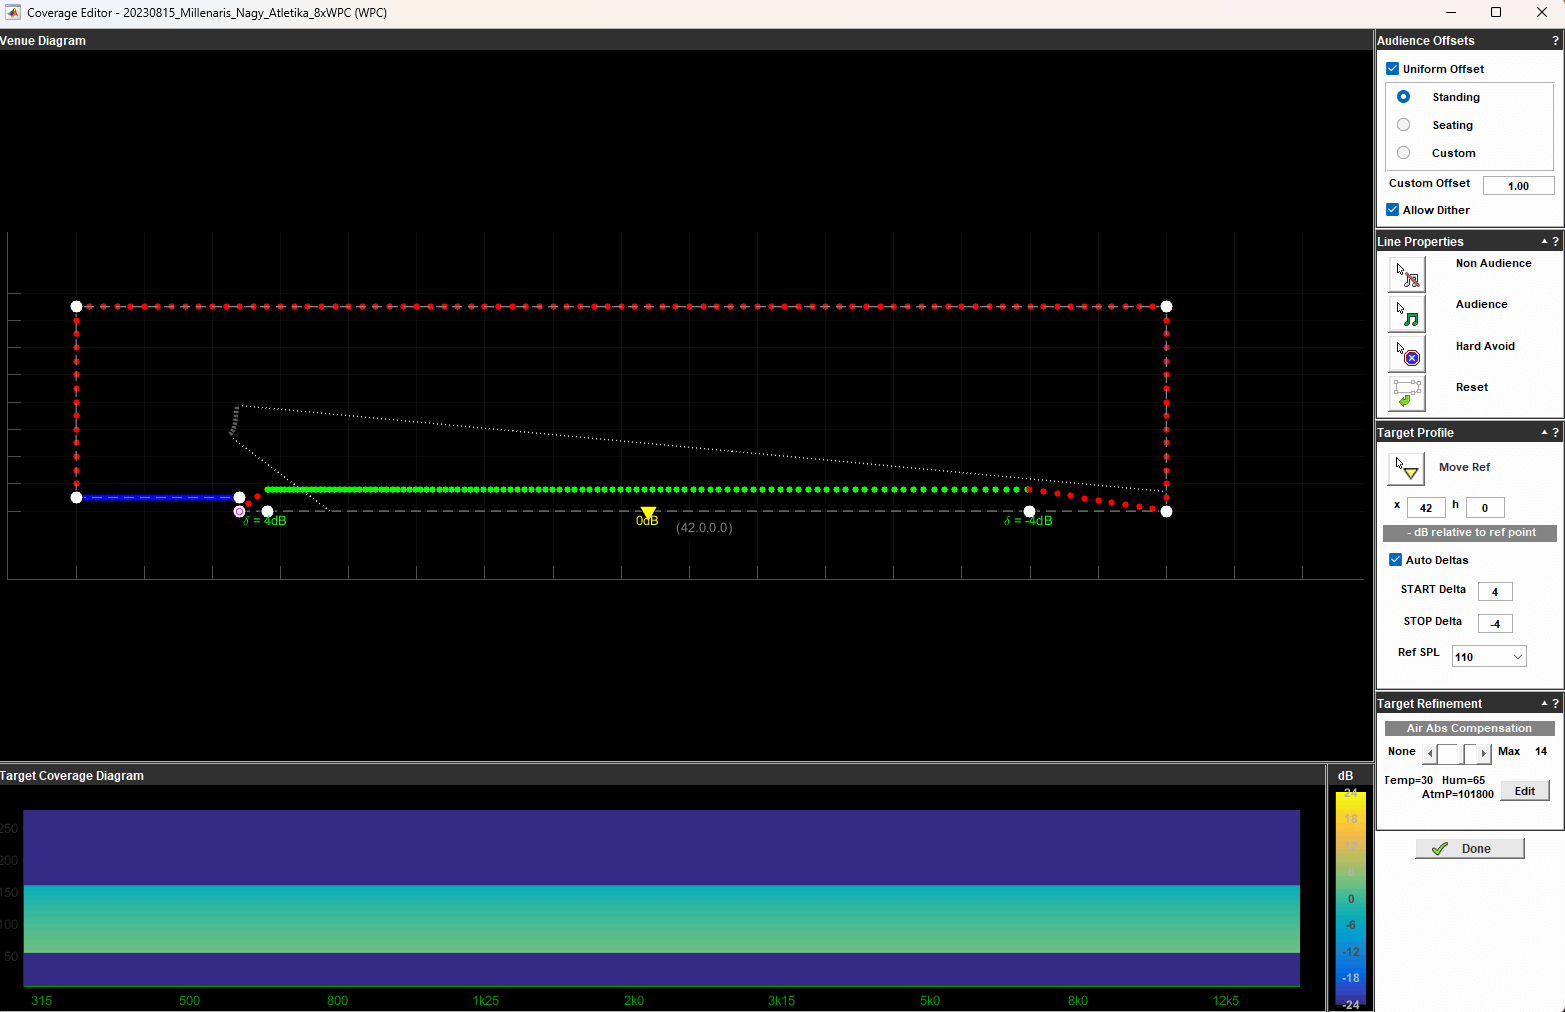
\includegraphics[width=\textwidth, keepaspectratio]{figures/display_wpc_2.png}
	\caption{Display 2.3.4 b1 \textit{``Cover''} kezelőfelülete (WPC)}\label{fig:display_wpc_2}
\end{figure}
%----------------------------------------------------------------------------
Miután a \textit{``Cover''} kezelőfelületen elvégeztük a szükséges beállításokat, a \textit{``Splay''} kezelőfelületen folytatjuk a tervezést.
Az optimalizáció ezen részén a hangrendszert fogjuk a hallgatóság területére irányítani, a fokolási szögek beállításával.
A szoftver által biztosított optimalizációs algoritmus a lehető legjobb lefedettségre törekszik a tervezett területen.
Lehetőség van az optimalizáció súlyozási tényezőinek beállítására, de jelen esetben a gyári beállításokat használtam.
Amennyiben módosítani szeretnénk a súlyozást a \textit{``Target'} és a \textit{``Leakage''} mezőkben tudjuk megadni a súlyozási tényezőket.
A \textit{``Target''} mezőben megadott érték a közönség terület súlyozása,
a \textit{``Leakage''} mezőben megadott érték pedig a közönség területén kívül eső szivárgás súlyozása.
Az \textit{``Alow Polish''} opció engedélyezi a szoftvernek, hogy egy második körben finom hangolja a splay szögeket az első próbálkozás után.
Ezt az opciót előnyös bekapcsolni, mivel a szoftver így pontosabb eredményt tud produkálni, ezért ezt a beállítást mindig használom.
A \textit{``Max Time''} mezőben megadhatjuk, hogy a szoftvernek mennyi idő álljon rendelkezésére az optimalizáció elvégzéséhez.
Mivel a mai modern számítógépek olyan gyorsak, hogy a szoftver általában 1-2 perc alatt elvégzi az optimalizációt, ezért ezt az értéket
nem szoktam módosítani. A \textit{``Max Time''} mezőben megadott érték másodpercben értendő.
%----------------------------------------------------------------------------
\begin{figure}[H]
	\centering
	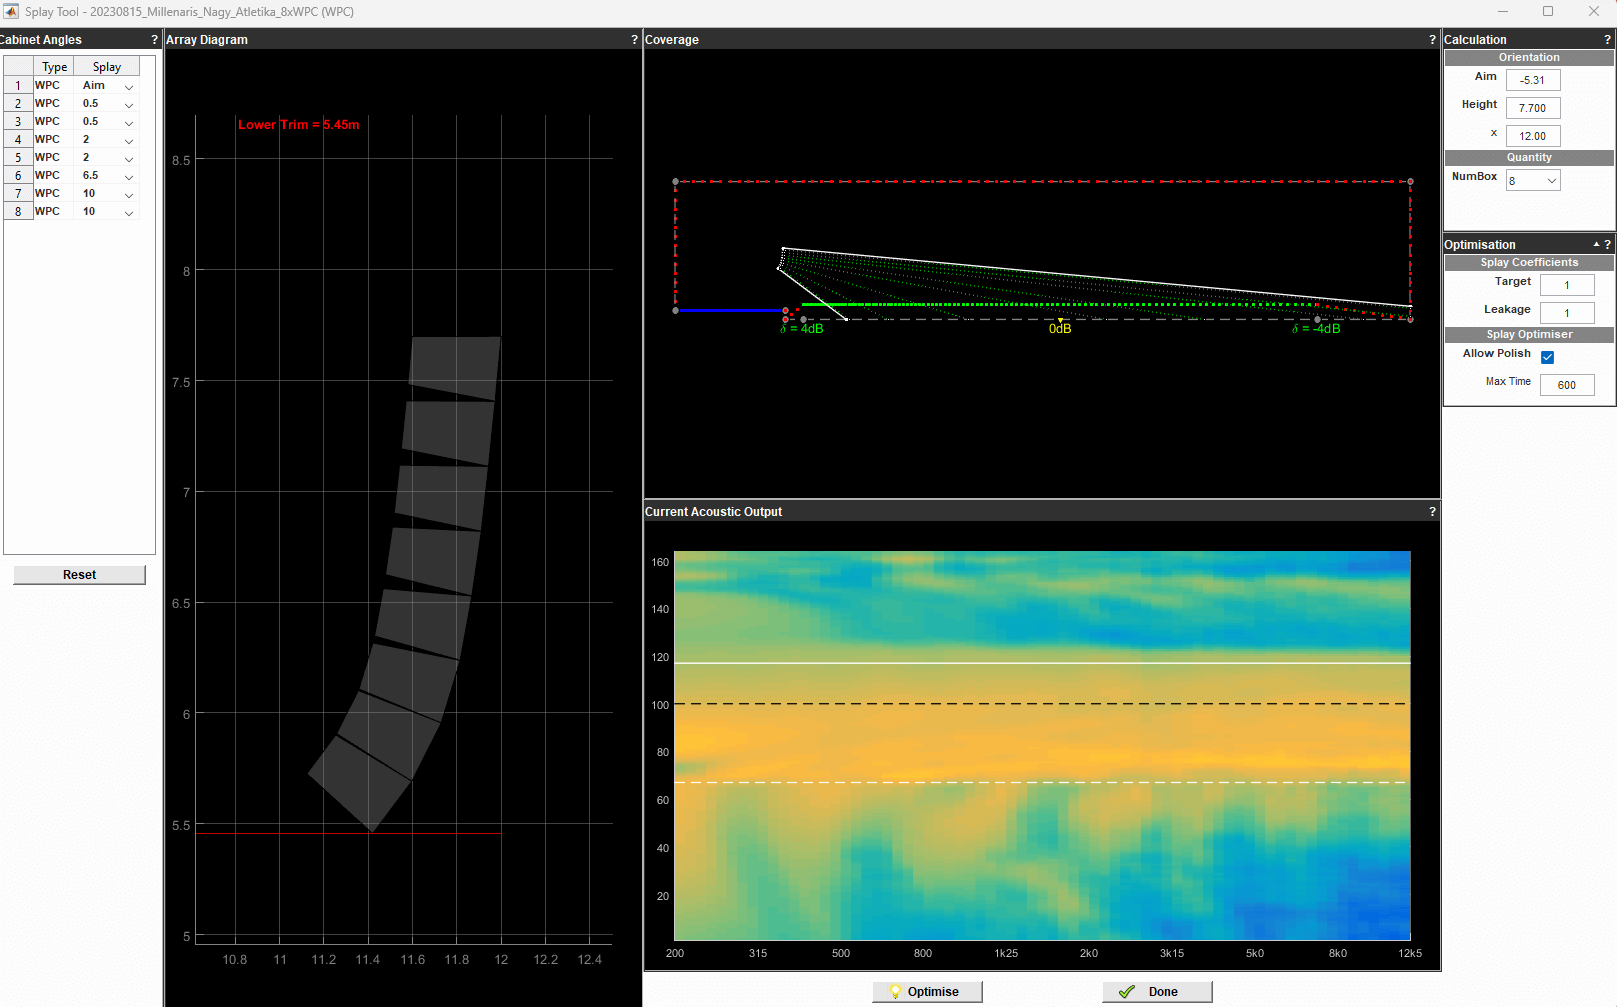
\includegraphics[width=\textwidth, keepaspectratio]{figures/display_wpc_3.png}
	\caption{Display 2.3.4 b1 \textit{``Splay''} kezelőfelülete (WPC)}\label{fig:display_wpc_3}
\end{figure}
%----------------------------------------------------------------------------
A következő lépés a \textit{``Rig''} kezelőfelületen történik. Ez a felület elsősorban az eddig elkészített
rendszerünket fogja megjeleníteni térben. Elsődleges beállítási paraméter ezen a panelen, hogy egy vagy két pontos
rögzítést szeretnénk-e használni. Jelen esetben egy pontos  rögzítést fogunk használni. Amennyiben valamilyen okból
szeretnénk változtatni a rendszer fizikai elhelyezkedésén, még megtehetjük, de ez a lépés ezen a ponton már nem ajánlott.
Bármely kis apró változtatás kardinálisan más végeredményhez vezethet. A tervezési folyamatot újra kell kezdeni, ellenkező esetben
a szoftver nem fogja tudni a megfelelő eredményt produkálni, és a rendszerünk nem úgy fog viselkedni a valóságban, ahogy azt mi szeretnénk.
A hangrendszer függesztéséhez és összeszereléséhez az összes információ megtalálható itt. Gondolva itt a riggvas fokolási helyére,
a ládák közti szögekre, a rendszer legfelső és legalsó pontjára.
Ezeken az információkon kívül még a rendszer súlyát és súlypontját is megkapjuk.
Esetünkben a teljes súly 289 kilogramm, amit a csarnok tartószerkezete biztonságosan elbír, valamint az egy tonnás emelőkapacitású
láncos emelők is képesek biztonságosan emelni. A súlypont a rendszer relatíve közepén helyezkedik el, ami stabil függesztést tesz lehetővé.
Ezek után a rendszert az említett paraméterek alapján össze építjük, figyelve az összes program által megadott információra.
%----------------------------------------------------------------------------
\begin{figure}[H]
	\centering
	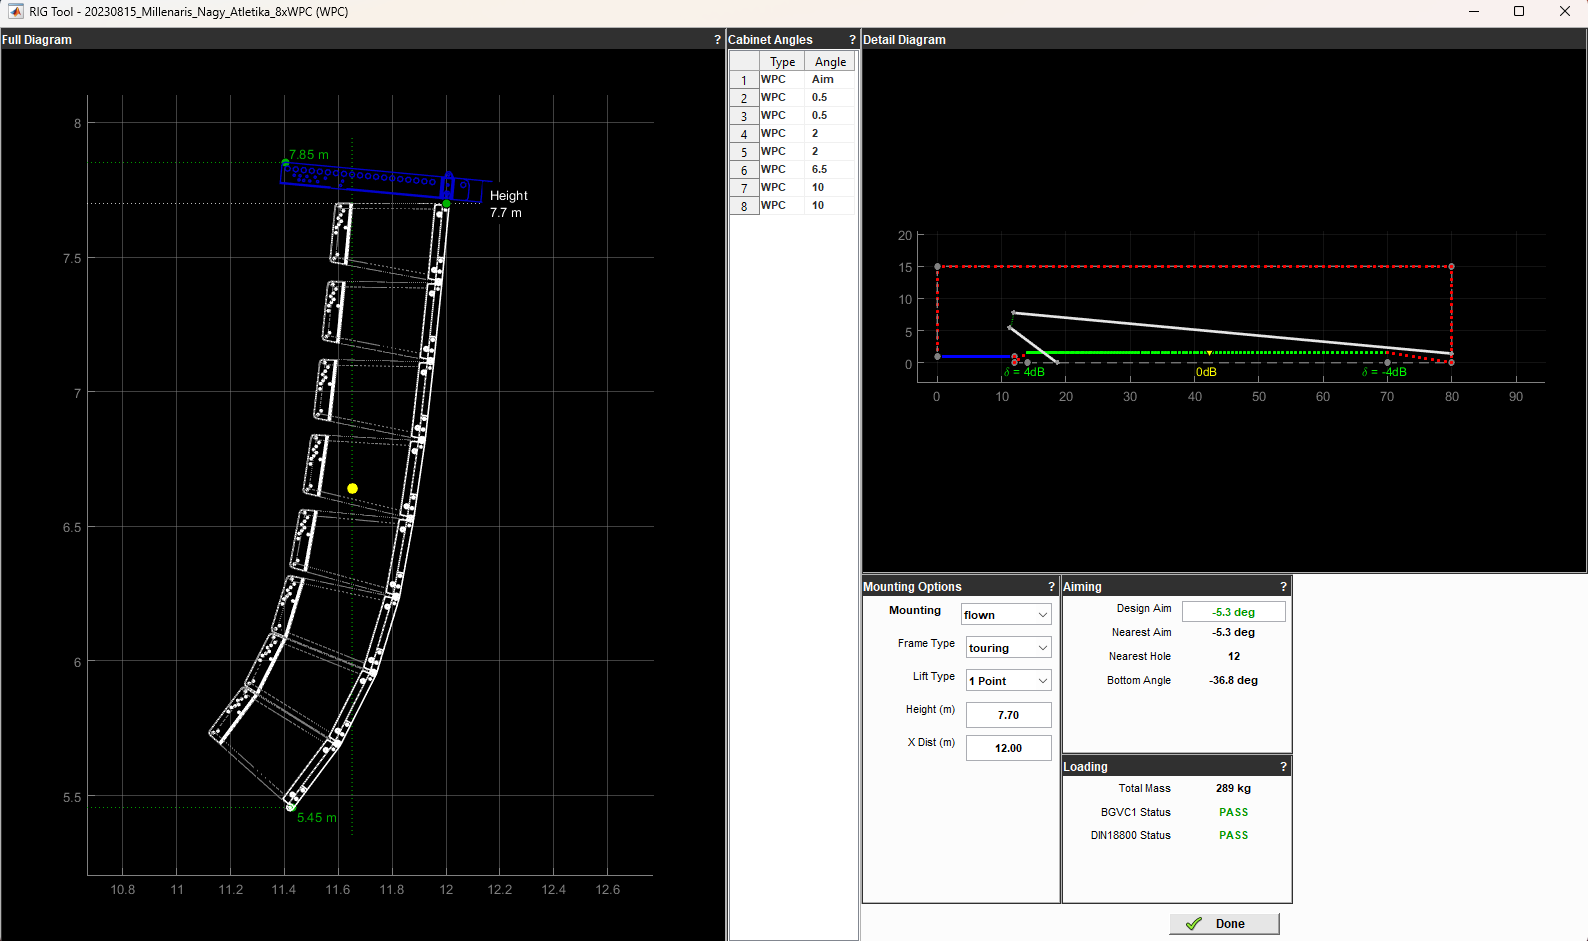
\includegraphics[width=\textwidth, keepaspectratio]{figures/display_wpc_4.png}
	\caption{Display 2.3.4 b1 \textit{``Rig''} kezelőfelülete (WPC)}\label{fig:display_wpc_4}
\end{figure}
%----------------------------------------------------------------------------
Az utolsó lépés mielőtt ki tudnánk menteni a tervezett rendszert, az a \textit{``EQ''} kezelőfelületen történik.
Ha a \textit{``Cover''} kezelőfelületen már megadtuk a környezeti változókat, akkor ezt már nem kell újra megtennünk,
mivel a szoftver automatikusan átveszi az ott megadott értékeket. Beállíthatjuk az alsó és felső határfrekvenciákat, de mivel
a program a kiválasztott hangrendszerhez tartozó gyári beállításokat automatikusan betölti, ezért ezeket az értékeket sem kell módosítani.
Amit viszont érdemes és erősen ajánlott módosítani, az a \textit{``Freq Res''} és a \textit{``Space Res''} értékek. Az előbbi a
frekvencia felbontást, az utóbbi pedig a térbeli felbontást jelenti. Ezek az értékek határozzák meg, hogy a szoftver milyen 
felbontásban végezze el a számításokat. Minél kisebb értéket adunk meg, annál pontosabb eredményt fogunk kapni, viszont a számítások
hosszabb ideig fognak tartani. A \textit{``Freq Res''} értékét 1-re, a \textit{``Space Res''} értékét pedig szintén 1-re állítottam, mivel
ez az elérhető legnagyobb felbontás, és a számításokat is a lehető legpontosabban szeretném elvégezni. A gyári érték mindegyiknél a kettő.
Minél pontosabbak a számítások, annál jobban fog viselkedni a rendszer a valóságban és egyenletesebb hangvisszaadást fog produkálni.
Ha már a kiegyensúlyozott hangvisszaadásnál tartunk, akkor a \textit{``Resolution''} panelen meg kell adnunk, hogy milyen
konfigurációban szeretnénk használni a rendszert. A WPC szériás hangládákat tudjuk akár egyesével hajtani, azaz egy láda egy végfok csatorna
párral (mivel Bi-Amp hangládáról beszélünk). De a gyártó lehetőséget biztosít arra is, hogy a ládákat párosával vagy hármasával is hajtsuk.
Ennek költséghatékonysági és rugalmassági előnyei vannak, viszont a hangvisszaadás kevésbé lesz egyenletes. Jelen esetben 
az arany középutat választottam, és párosával fogom hajtani a ládákat. Így a rendszer összesen 3 darab iK42 végfokot fog igényelni, ami 
12 darab végfokcsatornát jelent. A WPC rendszer csak iK42 végfokkal hajtható, a 8 csatornás iK81 végfokkal nem kompatibilis.
Lehetőség van az optimalizációs algoritmus befolyásolására is, a három előbbiekben már definiált súlyozási tényezők segítségével.
A fő hangsúlyt a \textit{``Target''} súlyozásra helyeztem, mivel a közönség területén szeretném a lehető legjobb hangvisszaadást elérni,
ezért 60\%-os súlyozást adtam neki.
A \textit{``Hard Avoid''} és a \textit{``Leakage''} súlyozását 20\%-ra állítottam.
Továbbá mindhárom résznek megadhatjuk mekkora hangnyomás értéket szeretnénk elérni a tervezett területen. Ezeket az értékeket
nem szükséges módosítani, mivel a gyári értékek megfelelőek, de ha mégis szeretnénk, akkor megtehetjük.
A paraméterezés után az optimalizáció után megkapjuk a teljes rendszer EQ beállítását és vizuális ábrázolást kapunk 
a referencia értéktől való eltérésekről.
%----------------------------------------------------------------------------
\begin{figure}[H]
	\centering
	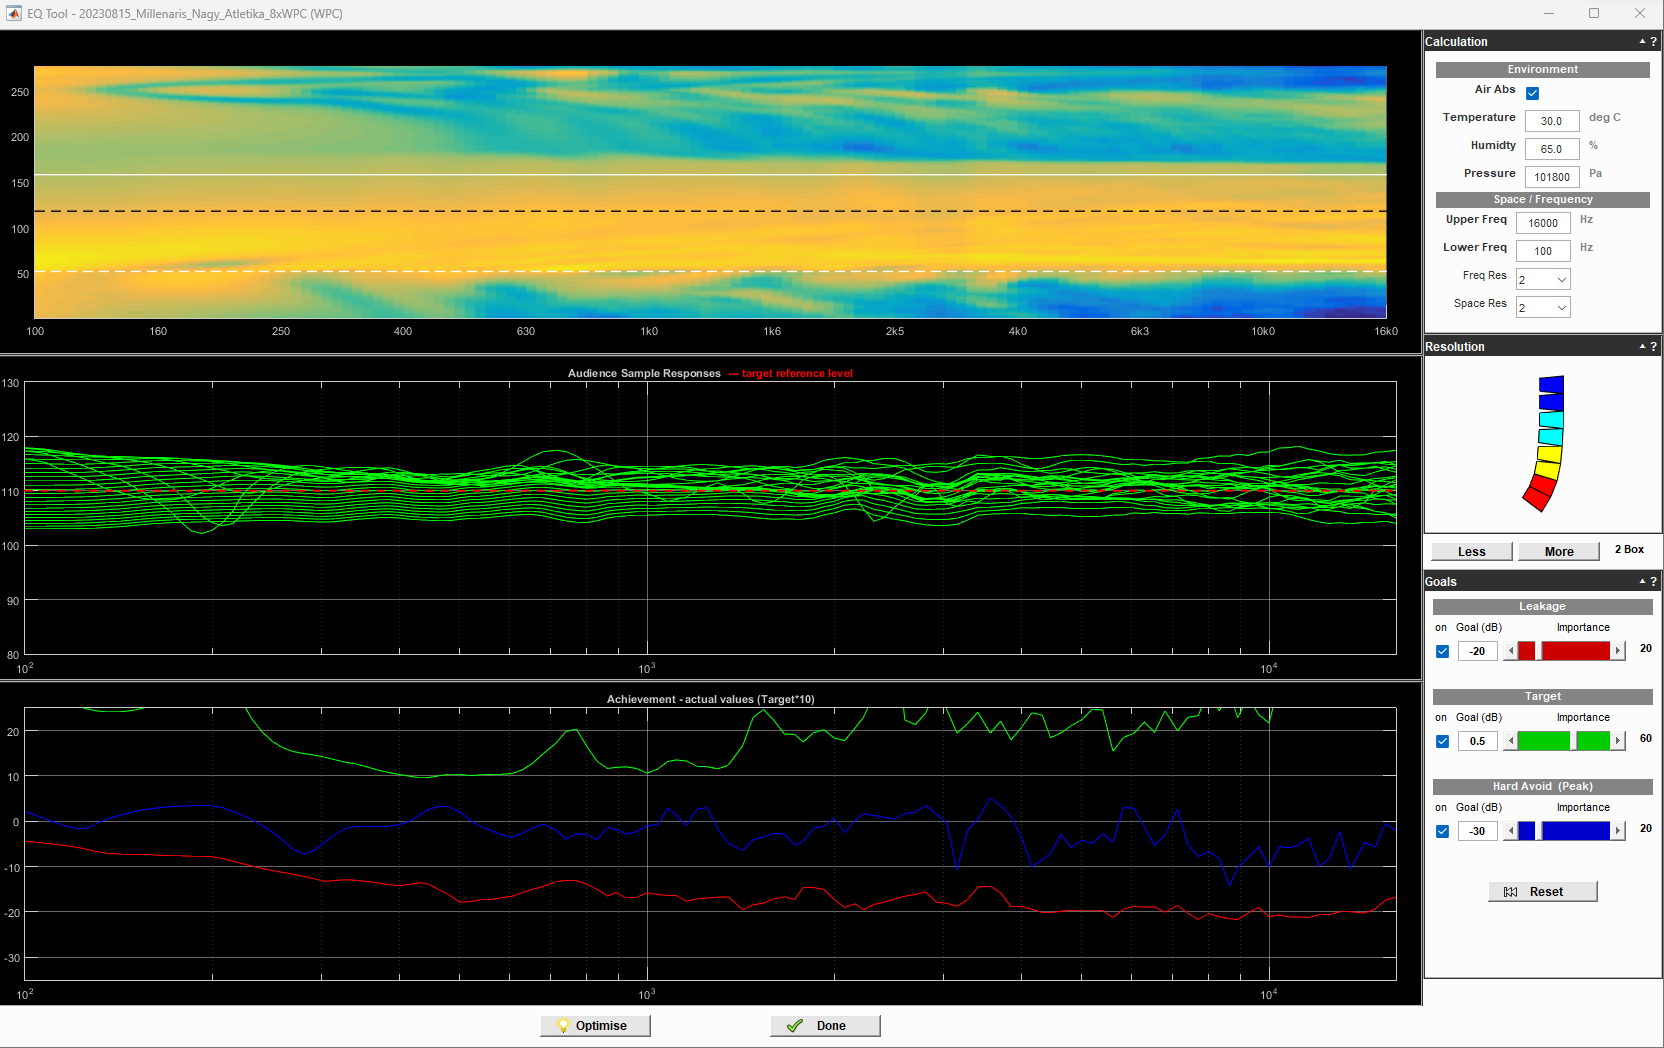
\includegraphics[width=\textwidth, keepaspectratio]{figures/display_wpc_5.png}
	\caption{Display 2.3.4 b1 \textit{``EQ''} kezelőfelülete (WPC)}\label{fig:display_wpc_5}
\end{figure}
%----------------------------------------------------------------------------
%Amennyiben szeretnénk megtekinteni a tervezett rendszer teljesítményét amit a program számított ki, 
%akkor az \textit{``SPL''} kezelőfelületen, az \textit{``Index Plot''}-on a bal egeret nyomva tartva
%tudunk virtuálisan mozogni a teremben, és megtekinthetjük a számított hangnyomás és frekvencia eloszlás értékeket.
%Ha mindent rendben találunk és nincsenek kivetnivalóink a tervezett rendszerrel kapcsolatban, akkor
%sikeresen megterveztük a hangrendszert, és elmenthetjük a projektet.
%A mentés során egy MAT kiterjesztésű fájlt fogunk kapni, segítségével később bármikor újra megnyithatjuk a projektet,
%ha ugyan azon a helyszínen dolgozunk, gyorsabban és egyszerűbben tudjuk a rendszert újra tervezni, a szükséges
%módosításokat elvégezni.
%----------------------------------------------------------------------------
%\begin{figure}[H]
%	\centering
%	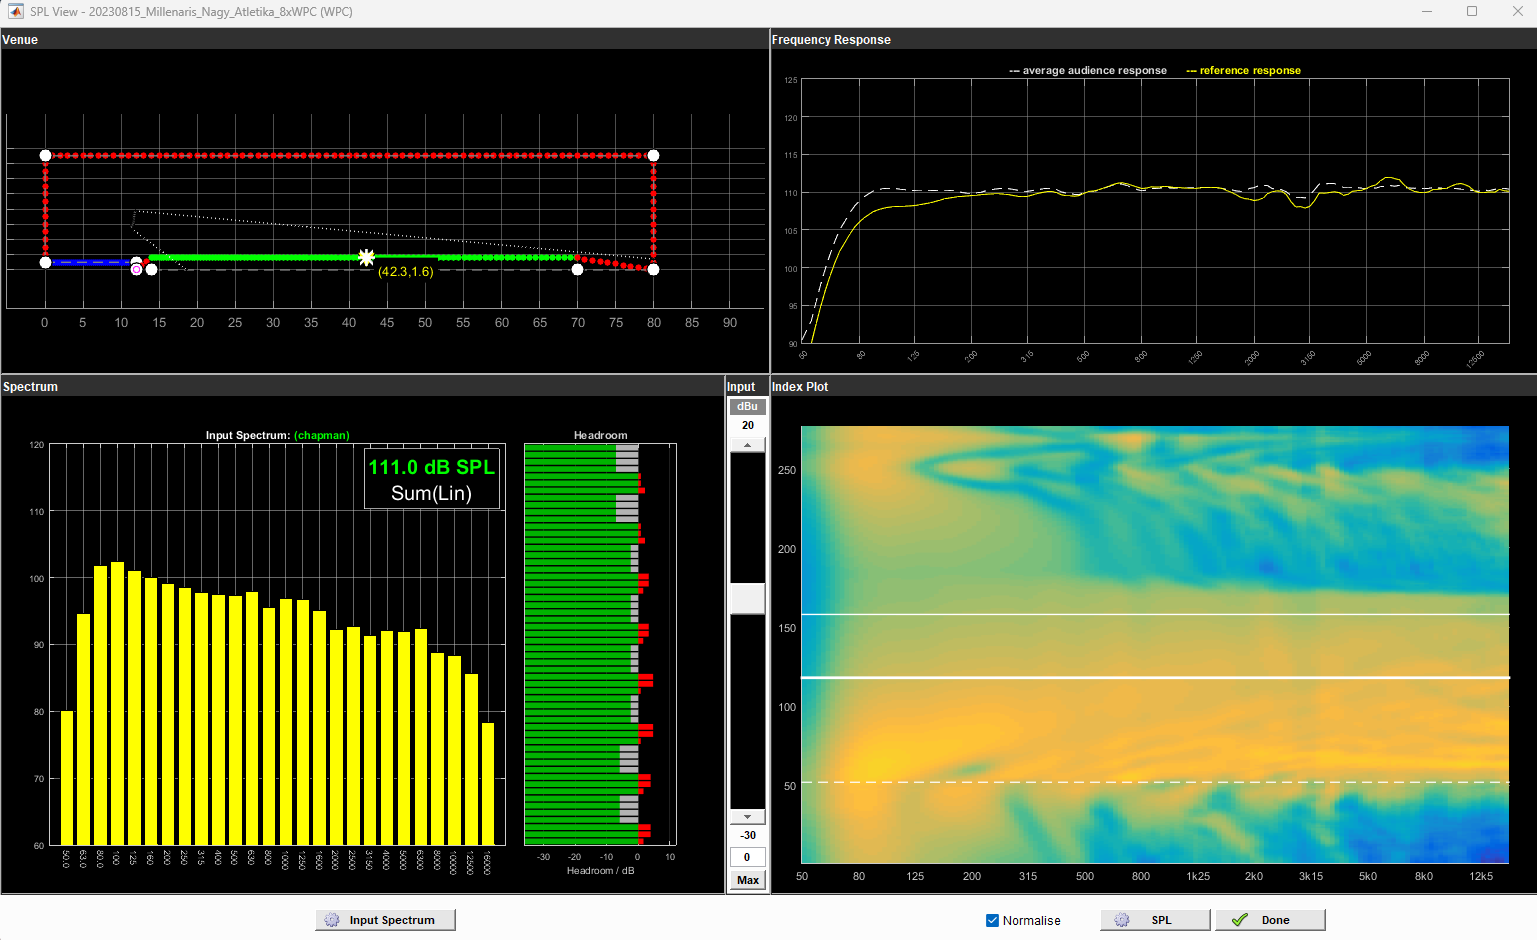
\includegraphics[width=\textwidth, keepaspectratio]{figures/display_wpc_6.png}
%	\caption{Display 2.3.4 b1 \textit{``SPL''}kezelőfelülete (WPC)}\label{fig:display_wpc_6}
%\end{figure}
%----------------------------------------------------------------------------
Az utolsó dolgunk ebben a programban mielőtt tovább lépünk, hogy exportáljuk a tervezett rendszert.
Az exportálás során egy D2P kiterjesztésű fájlt fogunk kapni, amit a VU-NET szoftver fog tud majd importálni a későbbiekben.
%----------------------------------------------------------------------------
\begin{figure}[H]
	\centering
	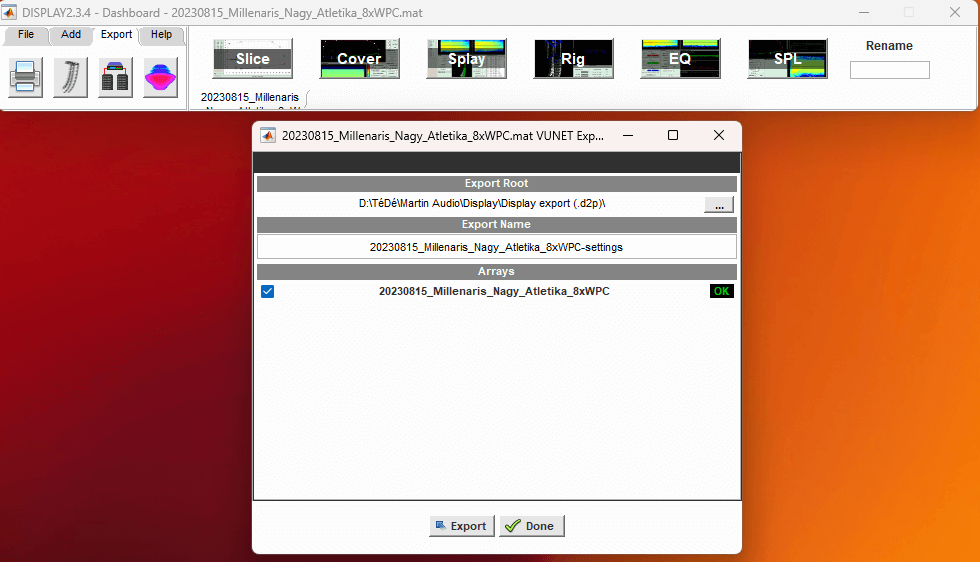
\includegraphics[width=\textwidth, keepaspectratio]{figures/display_wpc_7.png}
	\caption{Display 2.3.4 b1 exportáló kezelőfelülete (WPC)}\label{fig:display_wpc_7}
\end{figure}
%----------------------------------------------------------------------------
A fő hangrendszer megtervezése után a következő részegység aminek a tervét el kell készíteni, az a Delay hangrendszer.
A Delay hangrendszer a fő hangrendszerrel együtt fog működni, és a közönségtér hátsó-közép részétől kezdve fogja kiegészíteni azt.
Erre azért van szükség, mert a csarnokban a közönség ezen része olyan távolságra helyezkedik el, hogy
a WPC rendszer már nem tudja a megfelelő hangnyomás szintet egyenletesen biztosítani.
Ezt a feladatot a Wavefront Precision sorozatból a WPM típusú hangládák fogják ellátni, oldalanként 6-6 darab LineArray modullal.
Ez a láda egy két utas passzív hangrendszer, 2 darab 6.5"-os mély hangszóróval (LF) és 3 darab 1.4"-es magas hangszóróval (HF). 
Maximásan 130 dB hangnyomás szintet tud biztosítani, nagy előnye ennek a fajta rendszernek a súly-teljesítmény aránya, mivel egy
darab láda mindössze 14 kilogramm. \cite{WPMUSERGUIDE}
%----------------------------------------------------------------------------
\begin{figure}[H]
	\centering
	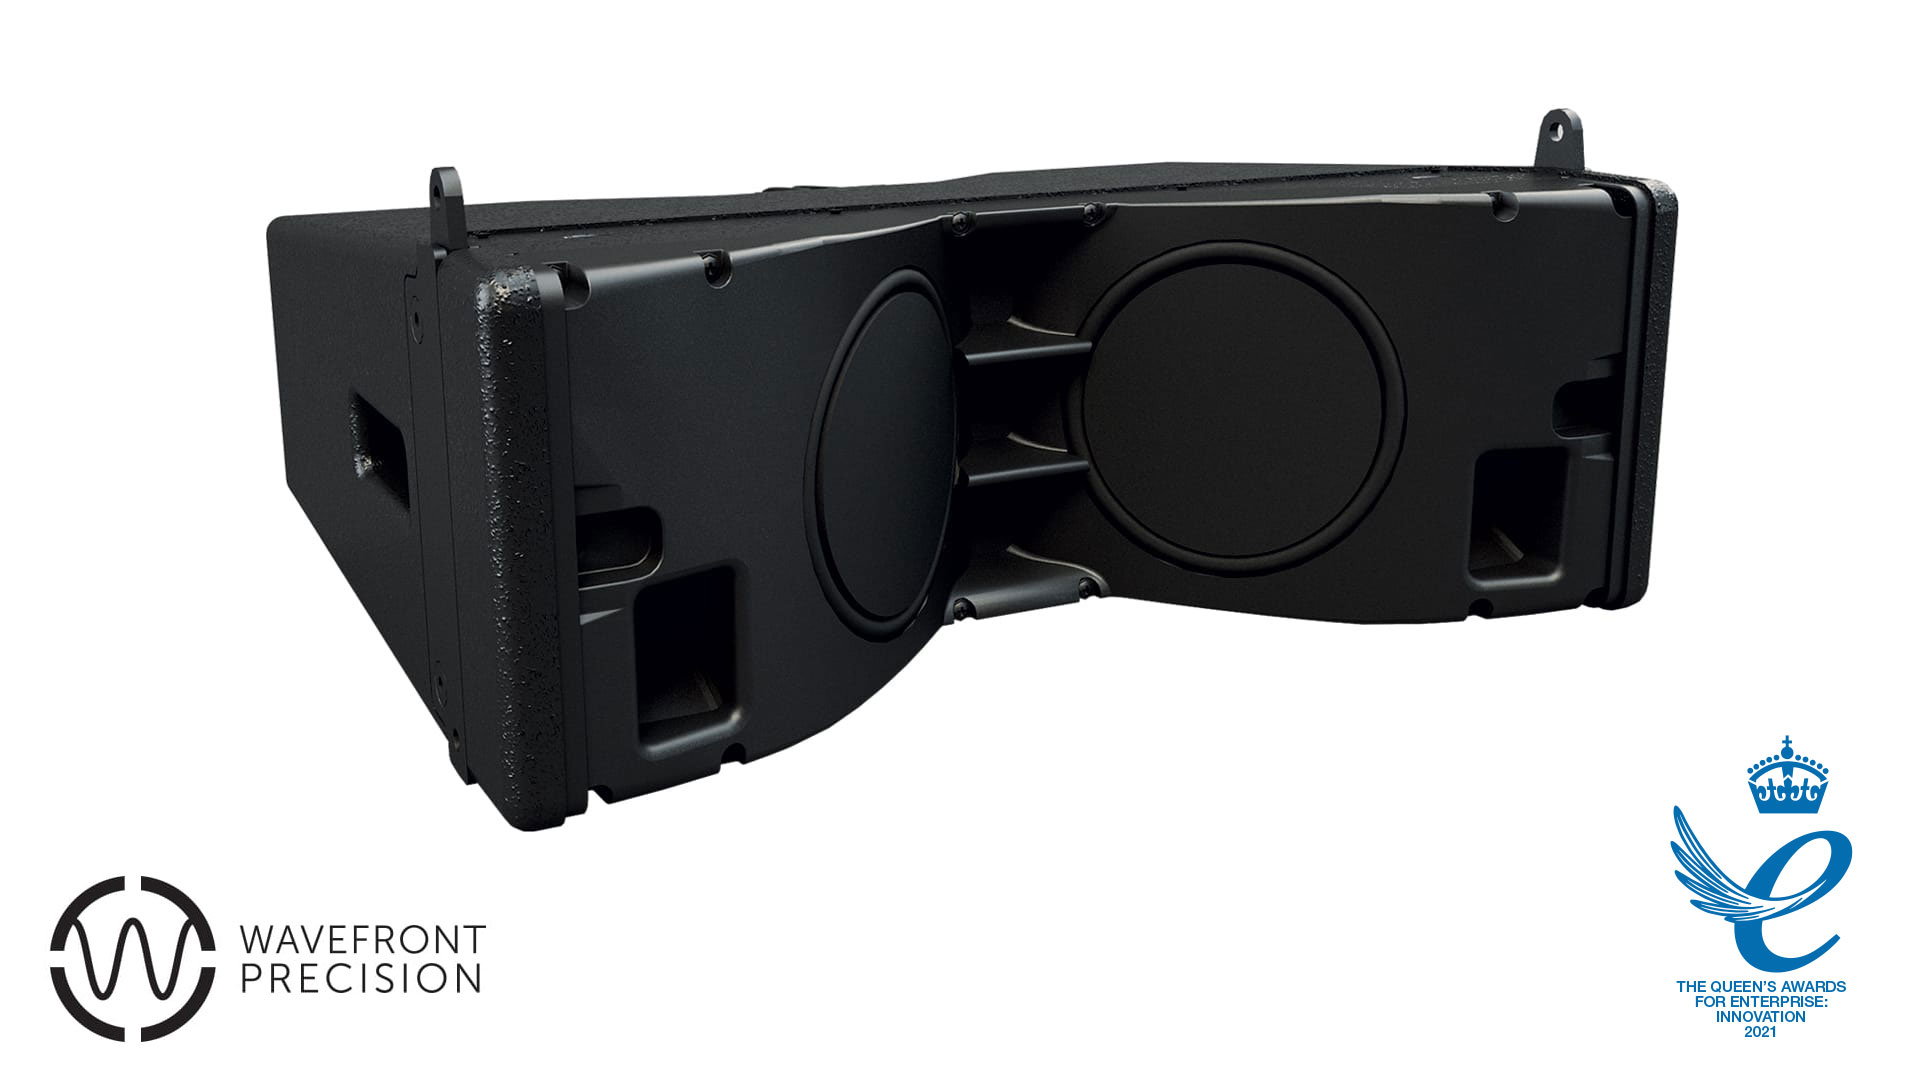
\includegraphics[width=80mm, keepaspectratio]{figures/wpm_front_view.jpg}
	\caption{Martin Audio WPM LineArray modul}\label{fig:wpm}
\end{figure}
%----------------------------------------------------------------------------
A tervezési fázisok nagy része megegyezik az előbbi rendszer tervezésével, ezért ezeket a részeket nem ismétlem meg.
A hangsúlyt a eltérésekre helyezem, és azokat fogom részletezni.
A fő különbség a \textit{``Cover''} kezelőfelületen történik, ahol a \textit{``Hard Avoid''} területet kell megjelölni.
Ezen a rajzon már radikálisan szükség van erre a funkcióra, mivel a közönség területén kívül eső területen beton nagy felületek találhatóak,
amelyek jelentős hangvisszaverődést okoznának. 
%----------------------------------------------------------------------------
%\begin{figure}[H]
%	\centering
%	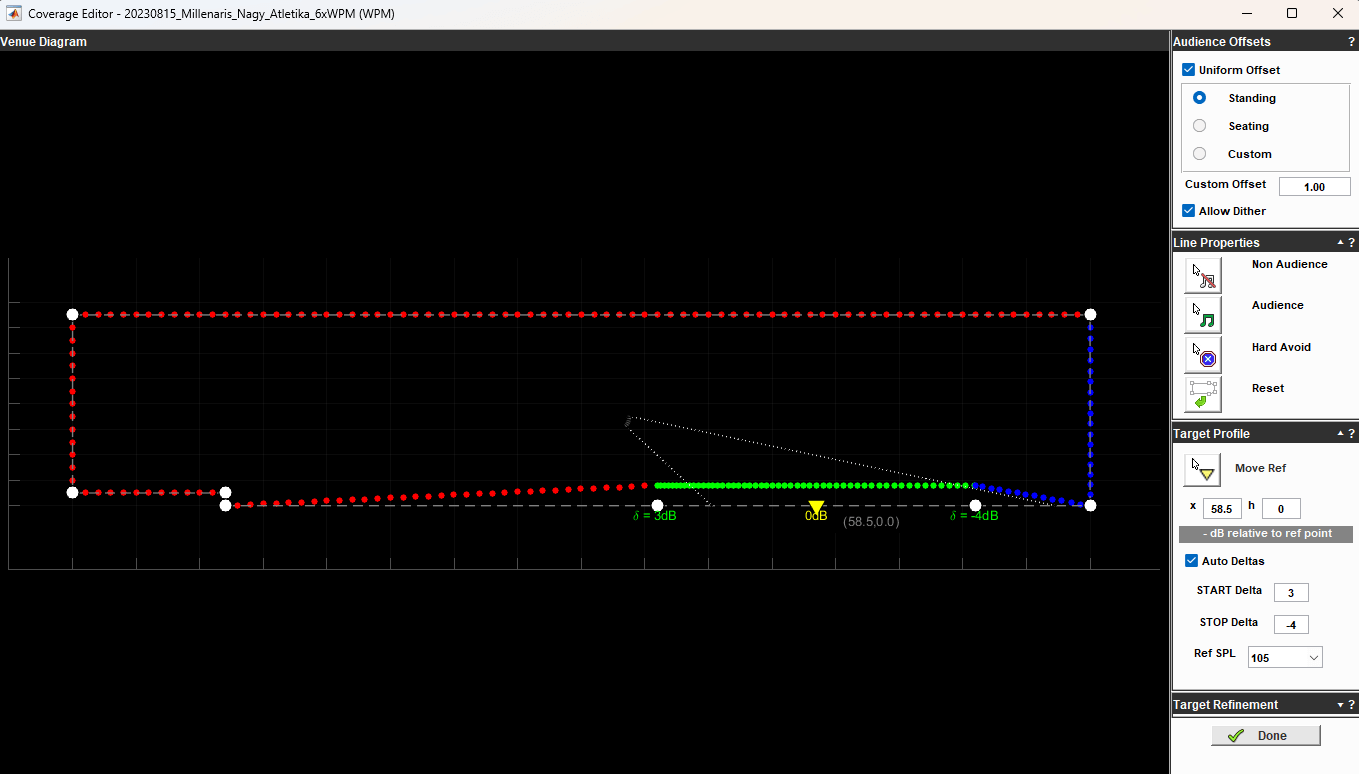
\includegraphics[width=\textwidth, keepaspectratio]{figures/display_wpm_1.png}
%	\caption{Display 2.3.4 b1 \textit{``Cover''} kezelőfelülete (WPM)}\label{fig:display_wpm_1}
%\end{figure}
%----------------------------------------------------------------------------
Ebből kifolyólag, szépen látható, hogy a program pontosan úgy optimalizálja a rendszert, hogy a \textit{``Hard Avoid''} területre, minél kevesebb
hangnyomás jusson.
Már a kék színnel jelölt terület első pár méterén radikálisan csökken a hangnyomás, és a rendszer a lehető legkevesebb energiát fordítja erre a területre.
A gyártó a WMP rendszert végfog csatornák szempontjából úgy tervezte, hogy a költség és a rugalmasság szempontjából akár négyesével is hajthatóak legyenek.
Ez persze nem jár kompromisszumok nélkül, a hangvisszaadás egyenletesebb lenne, ha egyesével hajtanánk a ládákat, de a jelenlegi rendszerben
hármasával fogom hajtani a ládákat, mivel ez a legköltséghatékonyabb megoldás, és végeredményben így is kielégítő hangvisszaadást fog produkálni mint 
kiegészítő egység.
%----------------------------------------------------------------------------
\begin{figure}[H]
	\centering
	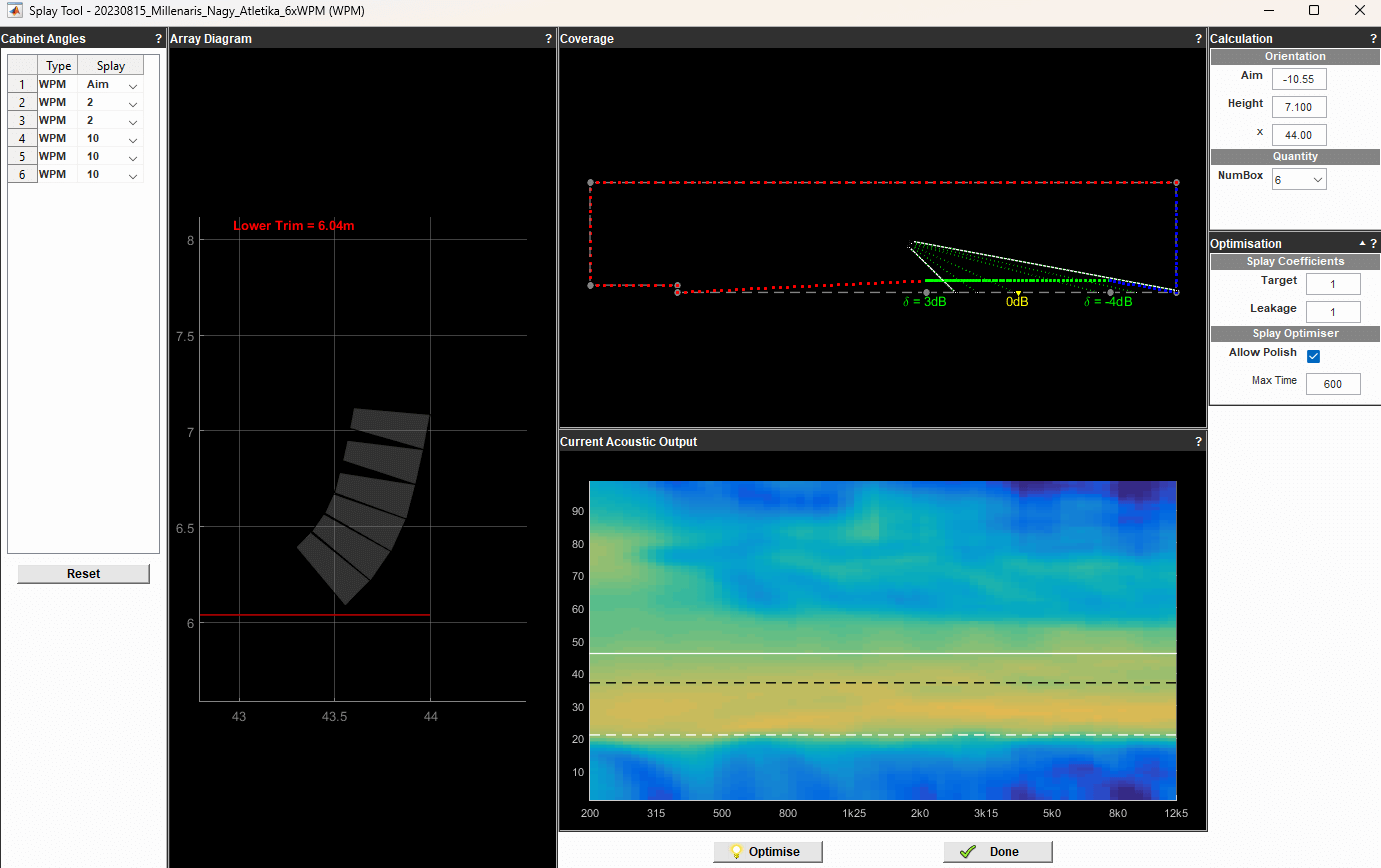
\includegraphics[width=\textwidth, keepaspectratio]{figures/display_wpm_2.png}
	\caption{Display 2.3.4 b1 \textit{``Splay''} kezelőfelülete (WPM)}\label{fig:display_wpm_2}
\end{figure}
%----------------------------------------------------------------------------
Az előbbiekben már tárgyalt exportáló felületen az összes többi optimalizációs lépést követően
mentjük az elkészített tervet a WPC rendszerhez hasonlóan.
%----------------------------------------------------------------------------
\subsubsection{Martin Audio VU-NET rendszer szoftver \cite{VUNETUSERGUIDE}}
%----------------------------------------------------------------------------
Miután már rendelkezünk az összes számunkra szükséges tervezett rendszerrel a rendezvényhez, a következő lépések a VU-NET szoftverben történnek.
A VU-NET szoftver egy olyan alkalmazás, amely lehetővé teszi a Martin Audio hangrendszerek teljes körű vezérlését és monitorozását.
Jelen esetben az iK42 és iK81 típusú végfokokat fogjuk tudni kezelni. 

%----------------------------------------------------------------------------
\subsubsection{Mélyláda rendszer}
%----------------------------------------------------------------------------
A mélyláda hangja hosszabb hullámhosszú, mint a többi komponensé, ezért az
optimális helymeghatározásuk és elhelyezésük kulcsfontosságú a megfelelő
hangzás érdekében. 
A rendszerben a Martin Audio SX218 típusú mélyládáit fogjuk használni.
Ezek a ládák dupla 18"-os mély hangszórókkal vannak felszerelve, 2000W AES és 8000W csúcsteljesítményre képesek, és
maximálisan 144 dB hangnyomás szintet tudnak biztosítani. \cite{SXSUBWOOFERUSERGUIDE}
Jelen esetben 12 darab ilyen láda fogja biztosítani a megfelelő mély tartományt a rendezvényen.
%----------------------------------------------------------------------------
\begin{figure}[H]
	\centering
	\includegraphics[width=80mm, keepaspectratio]{figures/sx218_front_view.jpg}
	\caption{Martin Audio SX218 mélyláda}\label{fig:sx218}
\end{figure}
%----------------------------------------------------------------------------
A \textit{``SUB''} tervezést egy általam készített Excel kalkulátor
segítségével végzem el. Ez a táblázat egyesíti a Martin Audio és Merlin van Veen által
készített kalkulátorokat (S.A.D), valamint kiegészítésre került további modulokkal és funkciókkal. \cite{MERLINVANVEEN} \cite{MARTINSUBCALCULATOR}
A egy EndFire konfigurációs mélyláda elrendezést terveztem. 
(Egy EndFire Pack = két láda egymás előtt adott távolságra és késleltetési értékkel) 
A táblázatba megadhatjuk, hogy éppen helyileg hol
van a rendezvény, és egy időjárás API segítségével megkapjuk az adott napra/napokra a
teljes időjárás előrejelzést. Majd ezekből egy adott időintervallumra átlagolva
megkapjuk az optimális értékeket a tervezéshez. 
A program kiszámolja, hogy milyen távolságra kell a ládákat helyezni egymástól előrefelé,
valamint mekkora \textit{``delay''} értéket kell alkalmazni. 
Majd az egyes EndFire Pack-ok egymáshoz képesti távolságot oldalirányban és azok
közötti delay értéket is megkapjuk. A \textit{``SUB array''}-t 63 Hz-re optimalizáltam, mivel
ez az a frekvenciatartomány, ahol a mélyláda rendszer a legtöbb energiát tudja leadni.
%----------------------------------------------------------------------------
\subsection{Allen \& Heath digitális keverőrendszer}
%----------------------------------------------------------------------------
A jelenlegi rendszer két keverőpultot fog tartalmazni, egyet a fő hangrendszerhez, és egyet a monitor rendszerhez.
Mindkét keverőpult Allen \& Heath SQ-6 típusú digitális keverőpult lesz.
A pultok 96 kHz-es mintavételezési frekvenciával operálnak és 48 csatornát képesek maximálisan kezelni, melyek közül 
24 csatornával rendelkezik fizikailag beépített mikrofon előerősítővel. A konzolokon található 16 programozható gomb,
25 fader melyek 6 rétegben helyezkednek el és a felhasználó személyre szabhatja őket a saját igényei szerint. 
Emellett 12 sztereó mix áll a rendelkezésünkre, melyeket szintén a felhasználó konfigurálhat saját igényei szerint.
A sztereóm mixek testreszabásával tudunk csoportokat is létrehozni.
A konzolokon 8 sztereó effekt motort is megtalálunk, ezekbe a virtuális effekt processzorokba a pultokon található ingyenes és fizetős 
pluginokat tudjuk betölteni. (amennyiben megvásároltuk a fizetős csomagokat, jelen rendszerben ezek nincsenek megvásárolva)
További előnye a platformnak, hogy egy 32x32 csatornás USB audio interfésszel rendelkezik, így a számítógéphez csatlakoztatva
egy nagy felbontású hangkártyaként is használhatjuk. \cite{AHSQ}
%----------------------------------------------------------------------------
\begin{figure}[H]
	\centering
	\includegraphics[width=80mm, keepaspectratio]{figures/sq6.jpg}
	\caption{Allen \& Heath SQ-6 digitális keverőpult}\label{fig:sq6}
\end{figure}
%----------------------------------------------------------------------------
Az I/O bővítőkártyák közül a rendszerben mindkét pultban megtalálható egy darab SQ Dante kártya ami 64x64 csatorna
kezelésére képes. Az A\&H SQ szériás pultjai csak egy darab I/O bővítőkártyát tudnak kezelni, de léteznek
olyan rendszerek mint például az Avantis és a DLive szériás pultok, amelyek több I/O bővítőkártyát is tudnak kezelni.
Jelen esetben ez teljes mértékben felesleges, mivel a rendszerben kizárólag a Dante protokollra támaszkodunk.

%----------------------------------------------------------------------------
\begin{figure}[H]
    \centering
    \begin{minipage}{0.45\textwidth}
        \centering
        \includegraphics[width=67mm, keepaspectratio]{figures/sq_dante.jpg}
        \caption{A\&H SQ Dante kártya}\label{fig:sq_dante}
    \end{minipage}\hfill
    \begin{minipage}{0.45\textwidth}
        \centering
        \includegraphics[width=67mm, keepaspectratio]{figures/dt168.jpg}
        \caption{A\&H DT168 Dante stagebox}\label{fig:dt168}
    \end{minipage}
\end{figure}
%----------------------------------------------------------------------------
\subsection{Shure ULXD digitális vezeték nélküli mikrofonrendszer}
%----------------------------------------------------------------------------
Manapság egy rendezvényen elengedhetetlen a vezeték nélküli mikrofonok használata.
%----------------------------------------------------------------------------
\subsection{Dante audio szerver}
%----------------------------------------------------------------------------
Ez a kiegészítő szerver egység lehetővé teszi bármilyen alacsony késleltetéssel dolgozó VST3 plugin használatát a rendszerben elő környezetben.
Olyan komplex funkcionalitásokat is elérhetünk, amelyek a keverőpulton csak limitáltan, vagy egyáltalán nem elérhetőek.
Gondolva itt a dinamikus EQ használatára, különböző kompressziós technikákra (például Opto, Multiband), 
A legnagyobb előnye ennek a fajta megoldásnak, hogy költségek szempontjából egy magasabb kategóriás keverőpult rendszer sokkal drágább lenne,
valamint nem vagyunk korlátozva a keverőpult által biztosított funkcionalitásokkal, bármikor tudunk igényeink szerint újabb és újabb pluginokat
telepíteni a rendszerbe, amíg a számítógép hardveres erőforrásai ezt lehetővé teszik.
Az általam épített szerver egy AMD Ryzen 7950X processzorral és 32 GB DDR5 memóriával, és a Focusrite RedNet PCIe kártya veszi fel a harcot a
komplex hangfeldolgozási feladatokkal. Ezekre a hardverekre azért esett a választás, mert mivel a Dante kártya 128 csatornát tud kezelni, 
(az épített rendszer 64 csatornás, de a bővítés lehetősége fent áll) erős számítási kapacitásra van szükség, hogy a rendszer a beállított
késleltetési értékek mellett is képes legyen késés nélkül a csatornák feldolgozására. Amennyiben nem sikerül a jelet a beállított időn belül
produkálni, furcsa zavaró pattogó hangokat hallhatunk, vagy rosszabb esetben hangkimaradás is előfordulhat. Ezért fontos a megfelelő hardveres
erőforrások biztosítása, és a pontos beállítások elvégzése.
A példában szereplő rendszer kifogástalanul képes elvégezni a feladatát, és a beállított 1 ms-os késleltetési értéket is képes folyamatosan tartani.
%----------------------------------------------------------------------------
\begin{figure}[H]
	\centering
	\includegraphics[width=67mm, keepaspectratio]{figures/rednet_pcie.jpg}
	\caption{Focusrite RedNet PCIe kártya}\label{fig:rednet_pcie}
\end{figure}
%----------------------------------------------------------------------------

%----------------------------------------------------------------------------
% !!! Képernyőfotó a szerverről !!!




%----------------------------------------------------------------------------
\subsection{Dante hálózat kialakítása és optimalizálása}
%----------------------------------------------------------------------------
\subsubsection{Dante Controller}
%---------------------------------------------------------------------------- 
% Hálózati mátrix
%----------------------------------------------------------------------------
Ezen a felületen tudjuk a hálózaton összekapcsolni a különböző hang vevőket és
adókat. Egy nagyobb rendszerben a konfigurálása rendkívül nagy odafigyelést és
precíziót igényel, pontosan tudnunk kell mit, hogyan és miért kötünk össze.
%----------------------------------------------------------------------------
% Eszköz nézet
%----------------------------------------------------------------------------
Mielőtt neki állnánk konfigurálni az adott eszközt, fontos eldöntenünk, hogy
milyen módban szeretnénk használni.
Lehetőségünk van két fő mód közül választani, a redundáns és a
váltott mód közül. A \textit{``redundant''} mód mint ahogy azt a neve is sugallja
redundáns kommunikációt valósít meg az eszközök között szoftveresen és
hardveresen egyaránt. Az összes Dante kártya a jelenlegi rendszerben gyári konfigurációban két RJ45-s
csatlakozóval rendelkezik. Jelen esetben ezt a módot választjuk az
üzembiztosság és a kritikus hibák minimalizálása miatt.
A másik lehetőség a \textit{``switched''} pedig eszközök láncolását
teszi egyszerűbbé. Amennyiben a redundancia nem elsődleges szempont számunkra, nem kell
minden egyes eszköz mögé switch, hanem a másodlagos RJ45 port direktbe köti
az arra csatlakoztatott eszközt az elsődleges hálózatra. Így gyorsabban és
költséghatékonyabban tudjuk kiépíteni a hálózatot, azonban a redundancia lehetősége megszűnik.
%----------------------------------------------------------------------------
\subsubsection{IP kiosztás}
%----------------------------------------------------------------------------
A rendszer képes automatikusan IP címeket osztani az egyes eszközöknek,
így meggyorsítva a munkafolyamatot.
Azonban egy fixen előre megtervezett rendszernél praktikusabb és
üzembiztosabb megoldás, ha minden eszköznek manuálisan megadjuk a címét a
hálózaton. A tervezett rendszerben minden egyes eszköznek fix IP címet adtam,
hogy könnyen és logikusan átlátható legyen az előbb említett előnyökön kívül.
A címeket egy online is elérhető Excel táblázatban tároltam, hogy amennyiben szükség van rá
bármikor könnyen elérhető legyen. Ez a táblázat a cégnél dolgozó összes munkatárs számára látható,
aki a rendszerrel foglalkozik. Így amennyiben új eszköz kerül a hálózatra, vagy egy eszköz IP címét
valamilyen okból meg kell változtatni, egyszerűen elérhető a szükséges információ.
%----------------------------------------------------------------------------
\begin{figure}[H]
	\centering
	\includegraphics[width=\textwidth, keepaspectratio]{figures/dante_ips.png}
	\caption{Dante eszközök IP címei a hálózaton}\label{fig:dante_ips}
\end{figure}
%----------------------------------------------------------------------------
%----------------------------------------------------------------------------
% Órajel nézet
%----------------------------------------------------------------------------
Meg kell adnunk az audio hálózatunk master órajelét. Ehhez az órajelhez
szinkronizál a többi eszköz.
Az időszinkronizáció kulcsfontosságú élőzenei produkcióknál.


%----------------------------------------------------------------------------
\subsection{Dante rendszer monitorozása}
%----------------------------------------------------------------------------



%----------------------------------------------------------------------------
% Hálózati állapot nézet
%----------------------------------------------------------------------------



%----------------------------------------------------------------------------
% Események nézet
%----------------------------------------------------------------------------



%----------------------------------------------------------------------------
\subsection{A rendszer mérése}
%----------------------------------------------------------------------------
A rendszermérések elkészítésére a Rational Acoustics által fejlesztett Smaart nevű szoftvert fogom használni, mivel
az iparágban ez a legelterjedtebb és legmegbízhatóbb szoftver a mérések pontos elvégzésére.
A szoftver legújabb verzióját fogom használni, ami az írás pillanatában a 'Smaart Suite 9.4.1' verzió.
Első lépésben a számítógéphez csatlakoztatott hangkártyát kell konfigurálni, hogy el tudjunk kezdeni méréseket végezni.
Jelen esetben a hangkártya maga a keverőpult, aminek az USB interfésze egy 32x32-es kapcsolatra képes a számítógéppel.
A mérőmikrofon egy Behringer ECM8000 típusú mérőmikrofon lesz, ami XLR csatlakozóval kapcsolódik a keverőhöz, a mikrofon tápellátását
a keverőpult biztosítja 48V fantomtáppal. Annak érdekében, hogy a mérés működőképes legyen, a mikrofont a keverőpulton be kell szintezni, minden 
processzálást kikapcsolni. A mikrofon kimenetét utána Direct Out móddal el kell küldeni az USB interfészre, ahol a Smaart szoftver
fogja tudni a jelet feldolgozni. Ezen kívül egy másik bemenetre is szükség lesz a keverőpulton, ahol a Smaart szoftver a referencia jelet fogja
küldeni, ezt szintén Direct Out módban vissza kell küldeni a számítógépre.
Tehát a példa kedvéért még egyszer:
Local Input 1: Behringer ECM8000 mérőmikrofon, majd Direct Out Output USB 1-re.
USB Input 1: Smaart szoftver referencia jele, majd Direct Out Output USB 2-re.


Az első mérés amit végezni fogok a rendszeren a mélyláda rendszer mérése lesz.
Az EndFire konfigurációban elhelyezett mélyláda rendszer mérése során a cél az, hogy maximalizáljuk a hangnyomást a közönség távolabbi részein is,
miközben hátrafelé kioltást érünk el. Ezen felül fontos a rendszer nyitása is, ha túl keskeny sávban működik, akkor a középső területek
hangnyomása túl magas lesz, a szélső területeken pedig túl alacsony. Tehát fel van adva a lecke, hogy a rendszer a lehetőségekhez mérten
egyenletes hangnyomást biztosítson a teljes területen.
Fontos, hogy a mérési környezet a lehetőségekhez mérten minél csendesebb legyen, valamint
ne legyenek olyan tárgyak a nézőtéren, amelyek a rendszer elő működése közben
nem lesznek jelen és mérés közben a mért hangot visszaverik. Ezzel minimalizálhatjuk a
hibákat és a mérések pontatlanságát, valamint a mérés reprezentatívabb lesz.




Mivel a mélyláda rendszer és a Main PA egymástól egy adott távolságra vannak, fontos, hogy a két rendszer fázishelyes és időhelyes legyen.


%----------------------------------------------------------------------------
\begin{figure}[H]
	\centering
	\includegraphics[width=\textwidth, keepaspectratio]{figures/smaart_sub_top.jpg}
	\caption{SUB - TOP mérések}\label{fig:smaart_sub_top}
\end{figure}
%----------------------------------------------------------------------------



%----------------------------------------------------------------------------
\subsection{A rendszer monitorozása}
%----------------------------------------------------------------------------


%----------------------------------------------------------------------------
\begin{figure}[H]
	\centering
	\includegraphics[width=\textwidth, keepaspectratio]{figures/smaart_spl_meter.jpg}
	\caption{SPL monitorozás a produkciók közben}\label{fig:smaart_spl_meter}
\end{figure}
%----------------------------------------------------------------------------
%----------------------------------------------------------------------------
\chapter{\FurtherDevelopment}
%----------------------------------------------------------------------------
\section{Üzemeltetési tapasztalatok és a végeredmény} % Konkrétan mely helyszíneken, hogyan zajlott, több tapasztalat megosztása, mi működött jól, és mi kevésbé.
%----------------------------------------------------------------------------
Ahogy már a modellezés során a korábbiakban említettem, a budapesti Millenáris B csarnoka 
volt a referencia helyszín, ahol a rendszert élesben telepítettem egy rendezvény idejére.
A képek magukért beszélnek, tökéletesen működött, a hangminőség kiváló volt, a hangnyomás szint pedig
a tervezett értékeknek megfelelően alakult. A mélyláda részegység és a Main PA LineArray fázishelyes és időben is helyes
volt, a frontfill kiegészítő késleltetése is megfelelően beállításra került, a teljes hangkép kiegyensúlyozott volt.
A rendszer működése során nem voltak hibák, stabilan működött a teljes rendezvény alatt. 
Nem voltak csomagvesztések a hálózaton, egyetlen egyszer sem kellett a másodlagos redundáns hálózatra váltani probléma miatt.
A szoftveres megoldások is kiválóan működtek, a számítógép stabilan futott a
rendelkezésre álló hardveres erőforrásokkal. A mérések is pontosak voltak, minden egységét
sikerült beállítani a megfelelő értékekre. 
A terem akusztikája alapvetően visszhangosnak mondható, mivel a teremben sok kemény felület található,
beton, fém és üveg felületek, amelyek a hangot visszaverik. Ehhez méghozzá járul a rendkívül magas belmagasság is,
ami szintén nem könnyítette meg a munkát. A tervezett rendszer azonban jól teljesített, a visszhangot sikerült minimalizálni,
és a legutolsó sorban is tisztán és egyenletesen hallható volt.
A fellépő zenekar és lemezlovas is meg volt elégedve, dicsérték nagy örömömre minden aspektusból.
Végül a megrendelő teljes mértékben elégedett volt a szolgáltatással, ezáltal 
a projekt sikeresnek mondható.
Összefoglalva minden komponens megfelelően végezte a rá bízott feladatot, és a rendszer
stabilan kihagyás nélkül működött a teljes üzemidő alatt. 
%----------------------------------------------------------------------------
\begin {figure}[H]
    \centering
    \includegraphics[width=300px]{figures/danci_wpc.jpg}
    \caption{A szakdolgozat szerzője a megépített WPC Line Array mögött emelés előtt}
\end {figure}
%----------------------------------------------------------------------------
\section{Továbbfejlesztési lehetőségek}
%----------------------------------------------------------------------------
\subsection{További eszközök integrálása}
%----------------------------------------------------------------------------
A Dante networking keresztrendszer lehetővé teszi a rendszerünk folyamatos bővítését a
hálózati limitációk megfelelő kezelésével. Bővítésekor figyelembe kell venni a
még rendelkezésre álló, a sávszélességet és a késleltetés mértékét. Amennyiben
tarjuk magunkat ezekhez a paraméterekhez, bővítése nem okozhat problémát,
és megfelelő overhead mellett elméletileg a teljes hálózatot is szaturálhatjuk mindenféle probléma nélkül.
A Martin Audio Wavefront sorozatú hangfalak skálázható felbontása lehetővé teszi, hogy
bővítésekor a már meglévő hangrendszerünket több végfokkal hajtva tovább
növeljük az egyenletes hangzást, a térbeli teljesítőképességet. Ez
javítja a rendszer hangminőségét, frekvenciafelbontását és az adott területen való
pontosabb hangeloszlást. Ebből kifolyólag nagy fejlesztés lehet a jövőben az egy ládás
felbontásra való kibővítés. Ez azt jelenti, hogy az összes Line Array egységet külön-külön
végfok csatornával hajtjuk meg.
További fejlesztés a rendszerben a LineArray hangfalak számának növelése megfelelő számú végfok egységgel,
amely tovább növeli az összeteljesítményt és a maximálisan lefedhető területet.
%----------------------------------------------------------------------------
\subsubsection{Shure Axient Digital rendszer} % A jel egyből a Dante hálózaton keresztül érkezik a keverőbe nincs A/D konverzió
%----------------------------------------------------------------------------
A Shure Axient Digital vezeték nélküli mikrofon szett a szakma egyik legjobb vezeték nélküli
mikrofonrendszere. Kiváló hangminőséget, megbízhatóságot és rugalmasságot kínál,
és a Dante hálózaton keresztül könnyen integrálható a már meglévő rendszerbe. A jelenlegi
Shure ULXD vezeték nélküli mikrofonjaink is kiváló minőségűek, azonban sajnálatos módon 
csak 48 kHz-es mintavételezési frekvenciával rendelkezik, míg az Axient Digital rendszer 96 kHz-es
mintavételezési frekvencián működik. Ezáltal a hangminőség jelentősen javulna a rendszerben,
valamint így integrálhatóvá válna direkt módon a Dante hálózaton keresztül a keverőbe, így
nem lenne szükség a hangot analóg jelekké alakítani, majd vissza. Ezáltal a hangminőség még 
kevésbé romlik.
Mint az eddigi Dante eszközünket, ezt is a Dante Controller segítségével könnyen konfigurálhatjuk, akár egy fixen
kijelölt csatornatartományban, amelyet a keverőpulton is könnyen beállíthatunk. Így mikor rendezvényre érkezünk,
plug and play módon azonnal használhatjuk a mikrofonokat, nem kell a csatornákat újra összepárosítani.
A Shure Wireless Workbench segítségével a mikrofonokat könnyen monitorozhatjuk, és a rendszer
állapotát is ellenőrizhetjük távolról is. Ez a bővítés jelentős költségekkel jár, így a
bővítés előtt alaposan mérlegelni kell, hogy valóban szükséges-e.
%----------------------------------------------------------------------------
\begin
    {figure}[H]
    \centering
    \includegraphics[width=70mm, keepaspectratio]{figures/axient_digital.png}
    \caption{Shure Axient Digital vezeték nélküli mikrofon rendszer}
    \label{fig:shure_axient_digital}
\end{figure}
%----------------------------------------------------------------------------
\begin{comment}
    
\subsubsection{TASCAM multitrack recorder} %TASCAM – DA-6400
%----------------------------------------------------------------------------
Egy másik fejlesztési lehetőség a rendszerben egy multitrack recorder beszerzése.
Ez a készülék lehetővé teszi a koncertek soksávos rögzítését, amelyeket később
visszahallgathatunk, vagy akár további feldolgozásra is továbbíthatunk. A TASCAM
DA-6400 egy 64 csatornás, 1U magas rackbe szerelhető multitrack recorder, amely
Dante hálózaton keresztül képes a hangot fogadni és rögzíteni. A felvétel
készítése során a hangot a Dante hálózaton keresztül kapja meg, így nem szükséges
a hangot analóg jelekké alakítani, majd vissza. Ezáltal a hangminőség nem romlik
a felvétel készítése során, és a felvétel készítése is egyszerűbb és gyorsabb lesz.
A felvétel készítése után a felvételt a TASCAM DA-6400-ról egy USB meghajtóra
menthetjük, majd további feldolgozásra továbbíthatjuk. 
%----------------------------------------------------------------------------
\begin
    {figure}[H]
    \centering
    \includegraphics[width=80mm, keepaspectratio]{figures/da_6400.jpg}
    \caption{TASCAM DA-6400 multitrack recorder}
    \label{fig:tascam_da_6400}
\end{figure}
%---------------------------------------------------------------------------- 
\end{comment}

\subsubsection{Allen \& Heath ME Personal Mixing System} % Előadóknak egyéni keverési lehetőség
%----------------------------------------------------------------------------
Az Allen \& Heath ME Personal Mixing System egy korszerű és kivételesen
rugalmas megoldás az előadók számára, amely lehetővé teszi az egyéni
monitorkeverést. Ez különösen fontos olyan helyzetekben,
ahol a színpadon több zenész dolgozik együtt, és mindegyikük
egyedi monitor igényekkel rendelkezik, ezek most már általában fülmonitorok.
Az Allen \& Heath ME rendszer három fő komponensből áll: a ME-U 
disztribúciós hubból, a ME-500 személyi keverőegységből, valamint a 
Dante hálózati kompatibilitást biztosító M-DANTE kártyából.
A ME-U egy 10 portos disztribúciós hub, amely lehetővé teszi több 
ME-500 keverőegység egyszerű és gyors csatlakoztatását. A rendszer egyik
kiemelkedő előnye, hogy minden csatlakoztatott eszköz egyetlen CAT5 
Ethernet kábelen keresztül kapja a tápellátást és az audiojelet is, ami
jelentősen egyszerűsíti a telepítést és az üzemeltetést. A ME-U támogatja 
a különböző digitális audió hálózati formátumokat, többek között a 
Dante protokollt is, amelyet az M-DANTE kártya biztosít.
Az M-DANTE kártya lehetővé teszi, hogy a ME rendszer integrálódjon 
a Dante alapú hálózati audió rendszerekkel.
%----------------------------------------------------------------------------
\begin{figure}[H]
    \centering
    \begin{minipage}{0.45\textwidth}
        \centering
        \includegraphics[width=50mm, keepaspectratio]{figures/me_u.jpg}
        \caption{A\&H ME-U disztribúciós hub}\label{fig:me_u}
    \end{minipage}\hfill
    \begin{minipage}{0.45\textwidth}
        \centering
        \includegraphics[width=50mm, keepaspectratio]{figures/m_dante.jpg}
        \caption{A\&H M-DANTE kártya}\label{fig:m_dante}
    \end{minipage}
\end{figure}
%----------------------------------------------------------------------------
\begin{comment}
\begin
    {figure}[H]
    \centering
    \includegraphics[width=65mm, keepaspectratio]{figures/me_500.jpg}
    \caption{Allen \& Heath ME-500 személyi keverőegység}
    \label{fig:martin_audio_wpl}
\end{figure}
\end{comment}
%----------------------------------------------------------------------------
%----------------------------------------------------------------------------
\subsubsection{Martin Audio WPL LineArray rendszer} % Nagyobb rendezvényekre
%----------------------------------------------------------------------------
Amennyiben egy sokkal nagyobb rendezvényről van szó, és a jelenlegi rendszerünk már nem
tudná lefedni a területet, akkor egy nagyobb szériás LineArray beszerzése is szükséges lehet. A
 Martin Audio WPL sorozatú ládái a jelenleg
elérhető legnagyobb terméke a Wavefront Precision sorozatban. 
Ebben az esetben a fő rendszert a WPL képviselné és WPC lenne az in-out fill.
A WPM szériás ládák pedig delayként szolgálnának a terület hátsó részén.
Viszont az említett teljes rendszerbővítésnek óriási költségei vannak, így bővítése előtt alaposan mérlegelni kell, megtérül-e a befektetés hosszabb távon.
%----------------------------------------------------------------------------
\begin
    {figure}[H]
    \centering
    \includegraphics[width=50mm, keepaspectratio]{figures/wpl_front_view.jpg}
    \caption{Martin Audio WPL LineArray modul}
    \label{fig:martin_audio_wpl}
\end{figure}
%----------------------------------------------------------------------------
\subsection{Bővítés nagyobb interfészre és keverőpultra}
%----------------------------------------------------------------------------
Tegyük fel, hogy egy szimfonikus zenekar koncertjét szeretnénk hangosítani, ahol a zenekar
tagjainak száma meghaladja a 64 főt és mindenki dedikált mikrofonnal rendelkezik. Ebben az
esetben a 64x64-es Dante interfész már nem elegendő, mivel a zenekar tagjainak száma
meghaladja a csatornaszámot. Ebben az esetben a rendszer bővítésére van szükség.
Így az Allen \& Heath SQ sorozatú keverőpultjai már nem elegendőek, mivel ezekbe a keverőkbe ez az interfész a maximális.
Ebben az esetben egy nagyobb csatornaszámú keverőpultot kell választanunk, amelyek közül a
az Avantis és a dLive sorozatú keverők jöhetnek szóba. Ezek már kaphatóak
128x128-as Dante interfésszel is, így megnövelve a csatornaszámot. Azonban ezek a keverők
jelentősen magasabb árkategóriába tartoznak, mint az SQ sorozatú keverők, így a bővítés
költsége is nagyobb lesz. A keverőpultok fejlesztése mellett szükséges további
stageboxokat is beszerezni az igényelt csatornaszám eléréséhez.
%----------------------------------------------------------------------------
\begin
    {figure}[H]
    \centering
    \includegraphics[width=60mm, keepaspectratio]{figures/dlive-s7000.jpg}
    \caption{Allen \& Heath dLive S7000 keverőpult}
    \label{fig:dLive_S7000}
\end{figure}
%----------------------------------------------------------------------------


% Köszönetnyilvánítás - opcionális
%~~~~~~~~~~~~~~~~~~~~~~~~~~~~~~~~~~~~~~~~~~~~~~~~~~~~~~~~~~~~~~~~~~~~~~~~~~~~~~~~~~~~~~
%----------------------------------------------------------------------------
\chapter*{\koszonetnyilvanitas}\addcontentsline{toc}{chapter}{\koszonetnyilvanitas}
%----------------------------------------------------------------------------




% Ábrák listája - a word-ös sablon szerint szükséges
%~~~~~~~~~~~~~~~~~~~~~~~~~~~~~~~~~~~~~~~~~~~~~~~~~~~~~~~~~~~~~~~~~~~~~~~~~~~~~~~~~~~~~~
\listoffigures\addcontentsline{toc}{chapter}{\listfigurename}


% Táblázatok listája - opcionális
%~~~~~~~~~~~~~~~~~~~~~~~~~~~~~~~~~~~~~~~~~~~~~~~~~~~~~~~~~~~~~~~~~~~~~~~~~~~~~~~~~~~~~~
\listoftables\addcontentsline{toc}{chapter}{\listtablename}


% Irodalomjegyzék
%~~~~~~~~~~~~~~~~~~~~~~~~~~~~~~~~~~~~~~~~~~~~~~~~~~~~~~~~~~~~~~~~~~~~~~~~~~~~~~~~~~~~~~
\addcontentsline{toc}{chapter}{\bibname}
\bibliography{bib/references}


% Függelékek
%~~~~~~~~~~~~~~~~~~~~~~~~~~~~~~~~~~~~~~~~~~~~~~~~~~~~~~~~~~~~~~~~~~~~~~~~~~~~~~~~~~~~~~
%%----------------------------------------------------------------------------
\appendix
%----------------------------------------------------------------------------
\chapter*{\fuggelek}\addcontentsline{toc}{chapter}{\fuggelek}
\setcounter{chapter}{\appendixnumber}
%\setcounter{equation}{0} % a fofejezet-szamlalo az angol ABC 6. betuje (F) lesz
\numberwithin{equation}{section}
\numberwithin{figure}{section}
\numberwithin{lstlisting}{section}
%\numberwithin{tabular}{section}

%----------------------------------------------------------------------------
\section{A TeXstudio felülete}
%----------------------------------------------------------------------------
\begin{figure}[!ht]
\centering
\includegraphics[width=150mm, keepaspectratio]{figures/TeXstudio.png}
\caption{A TeXstudio \LaTeX-szerkesztő.} 
\end{figure}

%----------------------------------------------------------------------------
\clearpage\section{Válasz az ,,Élet, a világmindenség, meg minden'' kérdésére}
%----------------------------------------------------------------------------
A Pitagorasz-tételből levezetve
\begin{align}
c^2=a^2+b^2=42.
\end{align}
A Faraday-indukciós törvényből levezetve
\begin{align}
\rot E=-\frac{dB}{dt}\hspace{1cm}\longrightarrow \hspace{1cm}
U_i=\oint\limits_\mathbf{L}{\mathbf{E}\mathbf{dl}}=-\frac{d}{dt}\int\limits_A{\mathbf{B}\mathbf{da}}=42.
\end{align}


%\label{page:last}
\end{document}